\documentclass[a4paper,headsepline=3pt,headinclude=true,12pt,oneside]{scrbook}
\usepackage[left=2cm,right=2cm,top=1cm,bottom=3cm,includeheadfoot]{geometry}
\usepackage{scrlayer-scrpage}
\usepackage{mwe}
\usepackage[origlayout=true,automark,colors={ph}]{URpagestyles}
\usepackage{lipsum} %fuer Fuelltexte

\usepackage{iftex}%automatische Auswahl des richtigen Fontloaders und der Eingabekodierung
%Es liefert das Makro \ifPDFTeX. Die Abfragen können entfernt werden, wenn nur eine bestimmte Variante verwendet wird.
\ifPDFTeX%falls mit pdfLaTeX kompiliert wird
	\usepackage[utf8]{inputenc}
	\usepackage[T1]{fontenc}
	\usepackage[ngerman]{babel} 
	%\usepackage[english]{babel} %Sparache aendern
\else%falls mit Lua oder XeLaTeX kompiliert wird
	\usepackage{fontspec}
	\usepackage{polyglossia}
	\setmainlanguage{german} 
	%\setmainlanguage{english} %Sprache aendern 
\fi
\usepackage{lmodern} %moderne Schriftarten
\usepackage{csquotes}
\usepackage{titletoc} %partielles Inhaltsverzeichnis

%alles mit Tabellen
\usepackage{array}
\usepackage{booktabs}
\usepackage{longtable}
\usepackage{csvsimple}
\usepackage{multirow}
\usepackage{makecell}

%\usepackage[dvipsnames]{xcolor} %Farben, optionen fuer mehr Voreinstellungen
%aufpassen beim Drucken, Drucker sind fast alle schlecht kalibriert, erst eine Testseite drucken

\usepackage{xspace} %Abstaende
\usepackage{setspace} %Zeilenabstand

%alles mit Bildern
\usepackage{float}
\usepackage{graphicx}
\usepackage{caption}
\usepackage{subcaption}
\usepackage{sidecap}
\usepackage{wrapfig}
\usepackage{pdfpages}

%alles mit Mathematik
\DeclareMathSizes{18}{18}{18}{18}
\usepackage{upgreek}
\usepackage{paralist}
\usepackage{amsmath}
\usepackage{amssymb}
\usepackage{amscd}
\usepackage[output-decimal-marker={,}]{siunitx}
\usepackage{thmtools}
\usepackage{pgfplots}
\pgfplotsset{compat=1.16}

%code texen
\usepackage{listings}
\lstset{ %Beispielkonfiguration fuer C-code
  backgroundcolor=\color{lightgray!50!white},   % choose the background color; you must add \usepackage{color} or \usepackage{xcolor}; should come as last argument
  basicstyle=\footnotesize,        % the size of the fonts that are used for the code
  breakatwhitespace=false,         % sets if automatic breaks should only happen at whitespace
  breaklines=true,                 % sets automatic line breaking
  captionpos=b,                    % sets the caption-position to bottom
  commentstyle=\color{orange},     % comment style
  deletekeywords={sizeof},         % if you want to delete keywords from the given language
  extendedchars=true,              % lets you use non-ASCII characters; for 8-bits encodings only, does not work with UTF-8
  firstnumber=1,                   % start line enumeration with line 1000
  frame=single,                    % adds a frame around the code
  keepspaces=true,                 % keeps spaces in text, useful for keeping indentation of code (possibly needs columns=flexible)
  %keywordstyle=\color{red!50!black},% keyword style
  keywordstyle=\color{blue},% keyword style
  language=C++,                    % the language of the code
  morekeywords={__constant__, __shared__, __device__, __host__, __global__, __managed__, float2, float3, float4, dim3, int2, int3, int4, uint, half, cudaStream_t, cudaEvent_t, cudaError_t, cudnnError_t, cusparseError_t, cublasError_t, curandError_t, cufftError_t, cusolverError_t, __kernel, kernel, __constant, constant, __local, local, __private, private, __global, global, cl_device_id, cl_platform_id, cl_int, cl_uint, cl_float, cl_double, string, cl_mem, cl_kernel, size_t, cl_event, cl_program, cl_context, cl_command_queue, FILE, restrict, event_t, ptrdiff_t , intptr_t, uintptr_t, device_ptr, device_vector, host_vector, vector, Platform, Context, CommandQueue, Buffer, Program, Kernel, Sources, Device, cl_context_properties, hipStream_t, cufftHandle, cufftComplex, cufftReal, cufftDouble, cufftDoubleComplex, clfftSetupData, clfftDim, fftw_complex, fftw_plan, curandStateSobol32_t, curandStateScrambledSobol32_t, curandStateSobol64_t, curandStateScrambledSobol64_t, curandState (XORWOW), curandStatePhilox4_32_10_t, curandStateMRG32k3a, curandStateMtgp32_t, curandGenerator_t, curandState, clrngMrg31k3pHostStream, clrngMrg31k3pStream, clprobdistExponential, clqmcLatticeRule, clqmcLatticeRuleStream, cublasHandle_t, cublasOperation_t, cuComplex, cuDoubleComplex, clsparseIdx_t, cldenseVector, clsparseCreateResult, clsparseCreateSolverResult, clsparseCsrMatrix, cusolverDnHandle_t, cusolverSpHandle_t, cusolverRfHandle_t, magma_queue_t, magma_int_t, LocalVector, CG, LocalStencil, __attribute__, aligned_allocator, auto, tensorflow, trt, tf, keras, Mat, cudnnHandle_t, cudnnTensorDescriptor_t, cudnnFilterDescriptor_t, cudnnConvolutionDescriptor_t, cudnnConvolutionFwdAlgo_t, ncclComm_t, MPI_INT},% if you want to add more keywords to the set
  numbers=left,                    % where to put the line-numbers; possible values are (none, left, right)
  numbersep=5pt,                   % how far the line-numbers are from the code
  numberstyle=\small\color{black}, % the style that is used for the line-numbers
  rulecolor=\color{black},         % if not set, the frame-color may be changed on line-breaks within not-black text (e.g. comments (green here))
  showspaces=false,                % show spaces everywhere adding particular underscores; it overrides 'showstringspaces'
  showstringspaces=false,          % underline spaces within strings only
  showtabs=false,                  % show tabs within strings adding particular underscores
  stepnumber=2,                    % the step between two line-numbers. If it's 1, each line will be numbered
  stringstyle=\color{green!50!black}, % string literal style
  identifierstyle=\color{black},
  tabsize=2,	                   % sets default tabsize to 2 spaces
  title=\lstname                   % show the filename of files included with \lstinputlisting; also try caption instead of title
}
\expandafter\ifx\csname li\endcsname\relax
\let\li=\lstinline
\else\errmessage{li schon definiert \meaning\li}%
\fi

%Literaturverzeichnis
\usepackage[backend=biber, citestyle=numeric, bibstyle=numeric]{biblatex}
\addbibresource{/home/kat10110/script/lit.bib} %richtigen Pfad ersetzen

%Index
\usepackage{makeidx}
\makeindex

\setlength{\parindent}{0pt} %keine Absatzeinzüge
\setlength{\parskip}{\baselineskip}

%Links
\usepackage[colorlinks=true,
            linkcolor=black,
            urlcolor=gray,
            citecolor=gray,
            bookmarks=true]{hyperref}
\usepackage{tabularx} %Tabellencounter, nach hyperref
\usepackage[toc,nopostdot]{glossaries} %Glossar, nach hyperref
\makeglossaries
\newglossaryentry{API}
{
	name=API,
	description={application programming interface, Programmierschnittstelle.},
	plural=APIs
}

\newglossaryentry{Arbeit}
{
	name=Arbeit,
	description={typischerweise eine Zahl von Flops, ein Maß für die Lesitung, die ein Programm erbringen muss.},
	plural=Arbeiten
}

\newglossaryentry{arithmetische Intensität}
{
	name=arithmetische Intensität,
	description={Verhältnis von Arbeit zum Datenverkehr.},
	plural=arithmetische Intensitäten
}

\newglossaryentry{Block}
{
	name=Block,
	description={ein evtl. mehrdimensionaler Verbund von Threads in Software (CUDA). Jeder Block besteht aus der gleichen Anzahl an Threads.},
	plural=Blöcke
}

\newglossaryentry{compute capability}
{
	name=compute capability,
	description={eine Versionsnummer der Chiparchitektur, die u.A. bestimmt, welche Features von CUDA auf der GPU implementiert wurden.},
	plural=compute capabilitys
}

\newglossaryentry{Command Queue}
{
	name=Command Queue,
	description={eine Menge von Instruktionen, die der Reihe nach abgehandelt werden sollen (OpenCL).},
	plural=Command Queues
}

\newglossaryentry{constant Memory}
{
	name=constant Memory,
	description={siehe erstes Vorkommen},
	plural=constant Memorys
}

\newglossaryentry{Datenverkehr}
{
	name=Datenverkehr,
	description={eine Zahl an Bytes, die während des Ausführens eines Programms insgesamt transferriert wird.}
}

\newglossaryentry{Gang}
{
	name=Gang,
	description={ein evtl. mehrdimensionaler Verbund von Vectors in Software (OpenACC). Jede Gang besteht aus der gleichen Anzahl an Vectors.},
	plural=Gangs
}

\newglossaryentry{global Memory}
{
	name=global Memory,
	description={siehe erstes Vorkommen},
	plural=global Memorys
}

\newglossaryentry{Grid}
{
	name=Grid,
	description={die Gesamtheit aller Blöcke (Nvidia).},
	plural=Grids
}

\newglossaryentry{Halfwarp}
{
	name=Halfwarp,
	description={ein Verbund von 16 Threads in Hardware (Nvidia, CUDA Terminologie).},
	plural=Halfwarps
}

\newglossaryentry{Handle}
{
	name=Handle,
	description={ein eindeutiger Referenzwert zu einer vom Betriebssystem verwalteten Systemressource.},
	plural=Handles
}

\newglossaryentry{Kernel}
{
	name=Kernel,
	description={eine kleine Recheneinheit, die auf die GPU ausgelagert werden soll.},
	plural=Kernel
}

\newglossaryentry{Kontext}
{
	name=Kontext,
	description={ein Handle für das OpenCL Programm (Speicherobjekte, Programs, Command Queues, ...).},
	plural=Kontexte
}

\newglossaryentry{local Memory}
{
	name=local Memory,
	description={Speicher (cached) eines einzelnen Threads (CUDA). \\ ein kleiner, sehr schneller Speicher, den sich alle Workitems einer Workgroup teilen (OpenCL). Pro SM wird einer verbaut (Nvidia).},
	plural=local Memorys
}

\newglossaryentry{MTIU}
{
	name=MTIU,
	description={Multi Threaded Instruction Unit, ein kleiner Controller, der Instruktionen an die Warps ausgibt.},
	plural=MTIUs
}

\newglossaryentry{nvcc}
{
	name=nvcc,
	description={Nvidia C(++) Compiler}
}

\newglossaryentry{nvlink}
{
	name=nvlink,
	description={eine High-Speed Datenschnittstelle für Nvidia Grafikkarten in Clustern.}
}

\newglossaryentry{NVPTX}
{
	name=NVPTX,
	description={Nvidia Parallel Thread Execution, eine assemblerartige Sprache, in die nvcc Devicecode übersetzt.}
}

\newglossaryentry{page-locked Memory}
{
	name=page-locked Memory,
	description={allozierter Speicher, der nicht vom Betriebssystem verschoben werden darf.}
}

\newglossaryentry{parallele Effizienz}
{
	name=parallele Effizienz,
	description={Verhältnis von Speedup zur Anzahl der eingesetzten Prozessoren.},
	plural=parallele Effizienzen
}

\newglossaryentry{PCIe}
{
	name=PCIe,
	description={Peripheral Component Interconnect Express, die standard-Schnittstelle für Steckkarten.}
}

\newglossaryentry{Peak Bandwidth}
{
	name=Peak Bandwidth,
	description={maximale interne Speicherbandbreite.},
	plural=Peak Bandwidth
}

\newglossaryentry{Peak Performance}
{
	name=Peak Performance,
	description={maximale Performance eines Prozessors.},
	plural=Peak Performances
}

\newglossaryentry{Performance}
{
	name=Performance,
	description={das Verhältnis von Flops zur benötigten Rechenzeit, ein Maß für die Effizienz von Soft- und Hardware.},
	plural=Performances
}

\newglossaryentry{Platform}
{
	name=Platform,
	description={eine OpenCL Imolementierung in Software.},
	plural=Platformen
}

\newglossaryentry{private Memory}
{
	name=private Memory,
	description={Speicher (cached) eines einzelnen Workitems (OpenCL).},
	plural=private Memorys
}

\newglossaryentry{shared Memory}
{
	name=shared Memory,
	description={siehe erstes Vorkommen},
	plural=shared Memorys
}

\newglossaryentry{SM}
{
	name=SM,
	description={Streaming Multiprocessor, Eine Recheneinheit bestehend aus mehreren Warps, einer MTIU und shared memory.},
	plural=SMs
}

\newglossaryentry{Speedup}
{
	name=Speedup,
	description={Faktor, um den ein paralleles Programm schneller läuft, als die sequentielle Variante.},
	plural=Speedups
}

\newglossaryentry{Stream}
{
	name=Stream,
	description={eine Menge von Instruktionen, die der Reihe nach abgehandelt werden sollen (CUDA).},
	plural=Streams
}

\newglossaryentry{texture Memory}
{
	name=Texture Memory,
	description={siehe erstes Vorkommen},
	plural=Texture Memorys
}

\newglossaryentry{Thread}
{
	name=Thread,
	description={die kleinste Recheneinheit einer GPU in CUDA, in Hardware auf Nvidia GPUs auch CUDA Core genannt.},
	plural=Threads
}

\newglossaryentry{Vector}
{
	name=Vector,
	description={die kleinste Recheneinheit einer GPU in OpenACC.},
	plural=Vectors
}

\newglossaryentry{Warp}
{
	name=Warp,
	description={Kombination zweier Halfwarps.},
	plural=Warps
}

\newglossaryentry{Wavefront}
{
	name=Wavefront,
	description={ein Verbund von 32 oder 64 Workitems in Hardware (AMD).},
	plural=Wavefronts
}

\newglossaryentry{Worker}
{
	name=Wavefront,
	description={ein Verbund von 32 Vectors in Hardware (Nvidia, OpenACC Terminologie).},
	plural=Workers
}

\newglossaryentry{Workgroup}
{
	name=Workgroup,
	description={ein evtl. mehrdimensionaler Verbund von Workitems in Software (OpenCL). Jede Workgroup besteht aus der gleichen Anzahl an Workitems.},
	plural=Workgroups
}

\newglossaryentry{Workitem}
{
	name=Workitem,
	description={die kleinste Recheneinheit einer GPU in OpenCL.},
	plural=Workitems
}
 %Glossardefinitionen einfuegen, richtigen Pfad ersetzen

\DeclareCaptionFont{black}{\color{black}}
\DeclareCaptionFormat{listing}{
  \colorbox[rgb]{1,1,1}{
    \parbox{\textwidth}{\hspace{15pt}#1#2#3}
  }
}
\captionsetup[lstlisting]{format=listing, labelfont=black, textfont=black, singlelinecheck=false, margin=0pt, font={bf,footnotesize}}

\renewcommand*{\familydefault}{\sfdefault}
\newcommand*{\pck}[1]{\texttt{#1}}
\newcommand*{\code}[1]{\texttt{#1}}
\newcommand*{\repl}[1]{\textrm{\textit{#1}}}
\newcommand{\cmd}[1]{\par\medskip\noindent\fbox{\ttfamily#1}\par\medskip\noindent}
\setcounter{secnumdepth}{\sectionnumdepth}
\newsavebox{\remarkbox}
\sbox{\remarkbox}{\emph{Anmerkung:~}}
\newcounter{iterator}
\usepackage{colortbl}

%meta Informationen
\author{Thomas Karl}
\title{Wissenschaftliches Rechnen auf Grafikkarten}
\subtitle{Universit\"at Regensburg}
\date{Sommersemester 2020}
\renewcommand{\titlepagestyle}{URtitle} 
\renewcommand{\lstlistingname}{Codebeispiel}
%\renewcommand{\thechapter}{\Roman{chapter}}
%\renewcommand{\thesection}{\thechapter~\arabic{section}}

\cfoot*{ }
\ofoot*{\thepage}% the pagenumber in the center of the foot, also on plain pages
\ihead*{ }% Name and title beneath each other in the inner part of the foot
\ohead*{\headmark}
\automark[subsection]{section}

\newcommand*\Laplace{\mathop{}\!\mathbin\bigtriangleup}

\begin{document}
\begin{onehalfspacing}
	\pagenumbering{Roman} %Die ersten Seiten roemisch nummeriert	

	\maketitle
	
	\includepdf{titlepage.pdf}	
	\newpage
	
	\tableofcontents
	\newpage
	
	\listoffigures
	\addcontentsline{toc}{chapter}{\listfigurename}
	\newpage
	
	\listoftables
	\addcontentsline{toc}{chapter}{\listtablename}
	\newpage
    
	\renewcommand{\lstlistlistingname}{Liste der Codebeispiele} %Listenname umbenennen
    \lstlistoflistings
    \addcontentsline{toc}{chapter}{\lstlistlistingname}
    \newpage
%    
    \printglossaries %Glossar automatisch im Inhaltsverzeichnis

%%%%%%%%%%%%%%%%%%%%%%%%%%%%%%%%%%%%%%%%%%%%%%%%%%%%%%%%%%%%%%%
%%%%%%%%%%%%%%%%%%%% eigentlicher Inhalt %%%%%%%%%%%%%%%%%%%%%% 
	\pagenumbering{arabic} %ab jetzt arabisch nummeriert
	\setcounter{page}{1} %beginnend mit eins, pdf-reader einstellen mit bookmarks=true in den Optionen von hyperref

    \startcontents[Einführung in High-Performance-Computing]
    \printcontents[Einführung in High-Performance-Computing]{l}{1}{\chapter*{Einführung in High-Performance-Computing}\setcounter{tocdepth}{2}}
    	\chapter{Einf\"uhrung in High-Performance-Computing} 
		\section{Amdahl's Law}
		Gegeben sei ein sequentielles Programm. Zerlegt man dieses in Teile, die theoretisch parallelisierbar sind, und jene, die in jedem Fall sequentiell laufen müssen, so ergibt sich die Gesamtlaufzeit $T$ als Summe 
		\begin{equation}\label{eq1:am}
		    T = t_p + t_s
        	\end{equation}
        	
        	wobei $t_p$ die Laufzeit des parallelisierbaren Anteils und $t_s$ die des sequentiellen bezeichnet. Zu den unparallelisierbaren Anteilen zählen typischerweise Prozessinitialisierung oder Speicherverwaltung. Benutzt man ferner Hardware zum Ausführen des Programms, auf der insgesamt $n_P$ Prozessoren oder Prozessorkerne dauerhaft zur Verfügung stehen, so gilt für den sogenannten maximalen Speedup $S$:
		\begin{equation}
		    S = \frac{T}{t_s + \frac{t_p}{n_p}} \leq \frac{T}{t_s} = \frac{T}{T-t_p}
        	\end{equation}	   
		
		Dabei wird das Verhältnis $\varepsilon = \frac{S}{n_P}$ auch als \gls{parallele Effizienz} bezeichnet. Als \Gls{Speedup} wird der Faktor bezeichnet, um den sich die Geschwindigkeit eines parallelen Programms gegenüber der sequentielle Vatiante verbessert. Abbildung \ref{1:am} zeigt diesen Speedup in Abhängigkeit von $n_p$ für verschiedene Verhältnisse von $\frac{t_p}{T}$.
		Allerdings hängt der sequentielle Anteil auch von der Parallelisierung selbst ab. Durch z.B. Prozessorkommunikation oder Synchronisation entsteht in der Gesamtlaufzeit ein zusätzlicher Summand	$t_{O(n_P)}$. In diesem Beispiel steigt der Anteil linear mit $n_P$. Dies ist jedoch nicht zwingend der Fall. Damit ergibt sich der maximale \Gls{Speedup}:		
		\begin{equation}
		    S = \frac{T}{t_s + t_{O(n_P)} + \frac{t_p}{n_p}} \leq \frac{T}{t_s} = \frac{T}{T-t_p}		
		\end{equation}
		
		Diese Kurve konvergiert nun nicht mehr gegen $\frac{T}{t_s}$, sondern erreicht ein Maximum, um danach wieder abzufallen (Abb. \ref{1:am_prax}). In der Praxis ergibt sich ein Optimum, eine Anzahl von Prozessoren, bei der sich der maximale \Gls{Speedup} erzielen lässt. Eine Vergrößerung dieser Anzahl hat einen negativen Effekt, da der Geschwindigkeitsgewinn durch die weiteren Prozessoren den Aufwand der Prozessorkommunikation nicht mehr kompensiert.


		\section{Gustafson's Law}
		Amdahl stellte mit seinem Gesetz eine worst-case Abschätzung auf, bei der sich die Laufzeit mit der Zahl der Prozessoren linear verbessern lässt. Amdahl geht dabei von einer festen Problemgröße aus. Gustafsons Gesetz hingegen geht von einem festen Zeitfenster aus. In diesem wächst die Problemgröße mit Anzahl der Prozessoren. Mit dieser Zahl wächst linear auch die Größe der Aufgabe, die unter den Voraussetzungen gelöst werden kann.

		Setzt man $P=t_p/T$ lässt sich \ref{eq1:am} umschreiben:
		\begin{equation}
			1 = (1 - P) + P
		\end{equation}
		
		Lässt sich der parallele Anteil unter Vernachlässigung von $t_{O(n_P)}$ gleichzeitig auf $n_P$ Prozessoren ausführen, so gilt für den \Gls{Speedup}:
    		\begin{equation}
        		S(n_P) = (1 - P) + n_P P
    		\end{equation}
		
		Der parallele Anteil wächst also linear mit der Anzahl der Prozessoren. Im Gegensatz zu Amdahl wird der sequentielle Anteil mit zunehmenden $n_p$ bedutungslos, wirkt also nicht beschränkend.
		 
		\section{Amdahl vs. Gustafson}		
		Nach Amdahl ist die \gls{parallele Effizienz}:
        	\begin{equation}
           	\varepsilon_{\text{Amdahl}}(n_P)    = \frac1{n_P}\cdot \frac1{(1-P)+P/n_P} = \frac1{n_P(1-P)+P}
        	\end{equation}
        	
        	Nach Gustafson ist die \gls{parallele Effizienz}:
		\begin{equation}
			\varepsilon_{\text{Gustafson}}(n_P) = 1 - \frac{n_P-1}{n_P}\cdot (1-P) = P +\frac{1-P}{n_P}
		\end{equation}
		
		Laut Amdahl geht die \gls{parallele Effizienz} im Limit einer großen Prozessorzahl immer gegen null, bei Gustafson existiert eine untere Schranke $P$:
		\begin{gather*}
			\lim\limits_{n_P \rightarrow \infty}\varepsilon_{\text{Amdahl}}(n_P)    = 0 \\        
			\lim\limits_{n_P \rightarrow \infty}\varepsilon_{\text{Gustafson}}(n_P) = P
		\end{gather*}
		
		Welches Modell nun Anwendung finden sollte, hängt von der Problemstellung ab. Gustafsons Gesetz sollte auf Probleme angewandt werden, falls sich die Promblemgrö\ss e auf die Parallelisierung anpassen lässt, andernfalls Amdahl. In jedem Fall geben Amdahl und Gustafson eine Ober- und Untergrenze für den \Gls{Speedup} an. 
        
		\begin{figure}[h]
		\centering
    		\includegraphics[height=0.4\textwidth]{chapter1/pictures/Amdahl_praxis.png}
    		\caption[Speedup laut Amdahl mit Prozesskommunikation]{Der Speedup laut Amdahl bei einer bestimmten Zahl an Prozessoren unter Berücksichtigung von Prozessorkommunikation. Ab einer bestimmten Anzahl nimmt der Speedup wieder ab. (doppelt-logarithmische Skala) \autocite{carch}}
    		\label{1:am_prax}
		\end{figure}
        
		\newpage
		\begin{figure}[h]
		\centering
    		\includegraphics[height=0.5\textwidth]{chapter1/pictures/Amdahl.png}
    		\caption[Speedup laut Amdahl ohne Prozesskommunikation]{Der Speedup laut Amdahl bei einer bestimmten Zahl an Prozessoren ohne Berücksichtigung von Prozesskommunikation für verschiedene Verhältnisse von $t_s/T$. Der Speedup konvergiert schnell gegen $T/t_s$. (einfach-logarithmische Skala) \autocite{wikiAmdahl}}
    		\label{1:am}
		\end{figure}
		
		\newpage
		\section{Roofline Model}
		\begin{figure}[t]
		\centering
	    	\includegraphics[height=0.4\textwidth]{chapter1/pictures/roofline_model_0.png}
    		\caption[Roofline Modell - naiv]{Die Performance $P$ als Funktion der arithmetischen Intensität $I$ bei doppelt-logarithmischer Skalierung. (naives Modell) \autocite{wikiRLM}}
    		\label{1:rl0}
		\end{figure}

		\begin{figure}[t]
		\centering
	    	\includegraphics[height=0.4\textheight]{chapter1/pictures/roofline_model_1.png}
    		\caption[Roofline Modell - \textit{bandwidth ceiling}]{Die Performance $P$ als Funktion der arithmetischen Intensität $I$ bei doppelt-logarithmischer Skalierung. Es existiert ein negativer Offset aufgrund von \textit{bandwidth ceiling}. Dieses Verhalten entsteht durch fehlende Speicheroptimierung. \autocite{wikiRLM}}
    		\label{1:rl1}
		\end{figure}
	
		\begin{figure}[t]
		\centering
	    	\includegraphics[height=0.35\textheight]{chapter1/pictures/roofline_model_2.png}
    		\caption[Roofline Modell - \textit{in-core ceiling}]{Die Performance $P$ als Funktion der arithmetischen Intensität $I$ bei doppelt-logarithmischer Skalierung. Es existiert ein e Beschränkung der \textit{peak performance} aufgrund von \textit{in-core ceiling}. \autocite{wikiRLM}}
    		\label{1:rl2}
		\end{figure}

		\begin{figure}[b]
		\centering
    		\includegraphics[height=0.35\textheight]{chapter1/pictures/roofline_model_3.png}
	    	\caption[Roofline Modell - \textit{locality walls}]{Die Performance $P$ als Funktion der arithmetischen Intensität $I$ bei doppelt-logarithmischer Skalierung. $I$ lässt sich aufgrund der Cachetopologie über bestimmte \textit{locality walls} hinaus nicht steigern. rechts: \textit{compulsory misses}, C3: zusätzlich \textit{capacity-} und \textit{conflict misses}, C2: zwei von drei \autocite{wikiRLM}}
    		\label{1:rl3}
		\end{figure}
		
		Sei eine \Gls{Arbeit} $W$ gegeben, die ein Programm oder auch nur eine bestimmte Funktion verrichten muss. $W$ wird üblicherweise angegeben in einer Zahl an Fließpunktoperationen (engl. floating point operations, FLOPs). Abhängig von der Problemstellung kann aber auch ein anderes Maß gewählt werden. $W$ ist eine Eigenschaft des Programms und hängt daher nur unwesentlich von der Hardware ab.
		
		Der \Gls{Datenverkehr} $Q$ (engl. memory traffic) bezeichnet die Zahl an Bytes, die während des Ausführens des Programms insgesamt transferriert wird. $Q$ ist im Wesentlichen eine Eigenschaft der Hardware und hängt z.B. von der Cachehierarchie ab.

		$I = W/Q$ bezeichnet die \gls{arithmetische Intensität}. Dabei handelt es sich um die Anzahl an Operationen pro transferriertes Byte. Die Einheit ist FLOPs/Byte.
		Das sogenannte naive Roofline Modell geht von nur zwei Parametern aus, der \textit{\Gls{Peak Bandwidth}} $\beta$ und der \textit{\Gls{Peak Performance}} $\pi$. Lediglich $I$ ist variabel. Die \textit{\Gls{Peak Performance}} ist eine feste Hardwaregröße, die vom ausführenden Gerät abhängt. Diese Größe lässt sich aus den entsprechenden Datenblättern ablesen. Die \textit{\Gls{Peak Bandwidth}} wird normalerweise durch \textit{benchmarking} bestimmt (später mehr). Die erreichbare \Gls{Performance} kann dann wie folgt berechnet werden:
		\begin{equation}
			P = \min \left\{ \begin{array}{ll} \pi \\
			\beta\times I \\ \end{array}\right.
		\end{equation}
		
		Abbildung \ref{1:rl0} zeigt dieses Verhalten exemplarisch. Der Schnittpunkt der beiden Linien $I^{\prime} = \pi/\beta$ wird als \textit{ridge point} bezeichnet und charakterisiert die eingesetzte Hardware entscheidend. Er bezeichnet jenes $I$, das ein Programm mindestens erreichen muss, um bei gegebener Hardware diese maximal auszureizen. Gleichzeitig beschreibt er den Punkt, ab der eine Erhöhung von $I$ keinen Effekt mehr hat. Bei Programmen, für die $I < I^{\prime}$ gilt, spricht man von \textit{memory bound}, andernfalls von \textit{compute bound}.
		
		Beim naiven Modell handelte es sich um eine best-case Abschätzung. In der Praxis gibt es allerdings weitere Limitierungen. Die Abbildungen \ref{1:rl1}, \ref{1:rl2} und \ref{1:rl3} zeigen folgende Fälle:
		
		\begin{enumerate}		
			\item Kommunikation: bandwidth ceilings
			\item Berechnung: in-core ceilings
			\item Lokalität: locality walls
		\end{enumerate}			
    \stopcontents[Einführung in High-Performance-Computing]
    
    \startcontents[Hardwaregrundlagen]
    \printcontents[Hardwaregrundlagen]{l}{1}{\chapter*{Hardwaregrundlagen}\setcounter{tocdepth}{2}}
		\chapter{Hardwaregrundlagen}
		\section{Flynn's Taxonomy}
		Aus Wikipedia \autocite{wikiFT}:
		
		Die Flynn’sche Taxonomie wurde 1966 von Michael J. Flynn publiziert und beschreibt eine grobe Unterteilung von Rechnerarchitekturen basierend auf der Anzahl der Befehls- (instruction streams) und Datenströme (data streams). Die Klassifikation teilt im Wesentlichen vier Bereiche ein:
		
		\begin{itemize}
		\item \textbf{Single Instruction, Single Data (SISD)}\\ Unter SISD-Rechnern versteht man traditionelle Einkernprozessor-Rechner, die ihre Aufgaben sequentiell abarbeiten. SISD-Rechner sind z. B. Personal-Computer (PCs) oder Workstations, welche nach der Von-Neumann- oder der Harvard-Architektur aufgebaut sind. Bei ersterer wird für Befehle und Daten die gleiche Speicheranbindung verwendet, bei letzterer sind sie getrennt. 
		
		\item \textbf{Single Instruction, Multiple Data (SIMD)}\\ Eine Architektur von Großrechnern beziehungsweise Supercomputern. SIMD-Computer, auch bekannt als Array-Prozessoren oder Vektorprozessor, dienen der schnellen Ausführung gleichartiger Rechenoperationen auf mehrere gleichzeitig eintreffende oder zur Verfügung stehende Eingangsdatenströme und werden vorwiegend in der Verarbeitung von Bild-, Ton- und Videodaten eingesetzt.

Dies ist sinnvoll, weil in diesen Bereichen die zu verarbeitenden Daten meist hochgradig parallelisierbar sind. So sind z. B. bei einem Videoschnitt die Operationen für die vielen einzelnen Bildpunkte identisch. Theoretisch optimal wäre hier die Ausführung durch einen einzigen, auf alle Punkte anzuwendenden Befehl.

Des Weiteren sind im Multimedia- und Kommunikationsbereich erforderliche Operationen häufig keine einfachen, einzelnen Operationen, sondern eher umfangreichere Befehlsketten. Das Einblenden eines Bildes vor einem Hintergrund ist beispielsweise ein komplexer Vorgang aus Maskenbildung mittels XOR, Vorbereitung des Hintergrundes mittels AND und NOT, sowie der Überlagerung der Teilbilder durch OR. Dieser Anforderung wird durch die Bereitstellung neuer komplexer Befehle entsprochen. So vereinigt z. B. der MMX-Befehl PANDN eine Invertierung und Und-Verknüpfung der Form x = y AND (NOT x).

Viele moderne Prozessorarchitekturen (wie PowerPC und x86) beinhalten inzwischen SIMD-Erweiterungen, das heißt spezielle zusätzliche Befehlssätze, die mit einem Befehlsaufruf gleichzeitig mehrere gleichartige Datensätze verarbeiten.

Allerdings muss man zwischen Befehlen unterscheiden, die lediglich gleichartige Rechenoperationen ausführen und anderen, die bis in den Bereich der DSP-Funktionalität hineinreichen (beispielsweise ist AltiVec in dieser Hinsicht wesentlich leistungsfähiger als 3DNow). 

    \item \textbf{Multiple Instruction, Single Data (MISD)}\\ Eine Architektur von Großrechnern bzw. Supercomputern. Die Zuordnung von Systemen zu dieser Klasse ist schwierig, sie ist deshalb umstritten. Viele sind der Meinung, dass es solche Systeme eigentlich nicht geben dürfte. Man kann aber fehlertolerante Systeme, die redundante Berechnungen ausführen, in diese Klasse einordnen. Ein Beispiel für dieses Prozessorsystem ist ein Schachcomputer.

Eine Umsetzung ist das Makropipelining, bei dem mehrere Recheneinheiten hintereinander geschaltet sind. Eine weitere sind redundante Datenströme zur Fehlererkennung bzw. -korrektur. 

    \item \textbf{Multiple Instruction, Multiple Data (MIMD)}\\ Eine Architektur von Großrechnern bzw. Supercomputern. MIMD-Computer führen gleichzeitig verschiedene Operationen auf verschieden gearteten Eingangsdatenströmen durch, wobei die Verteilung der Aufgaben an die zur Verfügung stehenden Ressourcen, meistens durch einen oder mehrere Prozessoren des Prozessorverbandes, selbst zur Laufzeit durchgeführt wird. Jeder Prozessor hat Zugriff auf die Daten anderer Prozessoren.

Man unterscheidet eng gekoppelte Systeme und lose gekoppelte Systeme. Eng gekoppelte Systeme sind Mehrprozessorsysteme, während lose gekoppelte Systeme Multicomputersysteme sind.

Multiprozessorsysteme teilen sich den vorhandenen Speicher und sind somit also ein shared-Memory System. Diese shared-Memory Systeme lassen sich weiter in UMA (uniform memory access), NUMA (non-uniform memory access) und COMA (cache-only memory access) unterteilen.

Man versucht bei MIMD eine Problemstellung durch die Lösung von Teilproblemen in den Griff zu bekommen. Dabei entsteht wiederum das Problem, dass verschiedene Teilstränge des Problems miteinander synchronisiert werden müssen.

Ein Beispiel in diesem Falle wäre das UNIX-Kommando make. Hier können auch mit mehreren Prozessoren mehrere zusammengehörige Programmcodes gleichzeitig in Maschinensprache übersetzt werden. 
        \end{itemize}
        
        \section{Aufbau einer Grafikkarte}
        Auch wenn das Moor'sche Gesetz noch ansatzweise erfüllt ist, stagniert die Leistung von einzelnen Prozessoren seit Jahren (Abb. \ref{2:hard}). Folglich versucht man viele Prozessoren zu einem großen Verbund zusammen zu schalten.
        
        \begin{figure}[h]
			\centering
    		    \includegraphics[width=0.8\textwidth]{chapter2/pictures/perf.pdf}
    		    \caption[Hardware]{Entwicklung der Hardware}
    		    \label{2:hard}
		\end{figure}
		
		\newpage

		Die Idee: nutze Grafikkarten als co-Prozessoren. Eine Grafikkarte besteht aus mehreren Teilen (Abb. \ref{2:graka}):
		\begin{itemize}
			\item \textbf{Bus Interface}: steuert den Datenfluss von der \Gls{PCIe}-Schnittstelle, Instruktionen werden an die GPU weitergeleitet, Speicherallozierungen an den Speichercontroller
			\item \textbf{Speichercontroller}: ein kleiner Mikroprozessor, der Speicher alloziert
			\item \textbf{Speicher}: beinhaltet den globalen und Texturspeicher. Die interne Speicherbandbreite liegt heutzutage bei bis zu 1TB/s (HBM2).
			\item \textbf{GPU}: das Herzstück der Grafikkarte. Ursprünglich war die einzige Aufgabe, der CPU 3d-Berechnungen für Texturen abzunehmen. Es existieren Grafikkarten mit zwei GPUs.
			\item \textbf{Video-Out-Controller}: wandelt die Berechnungen der GPU in Signale für die Videoausgänge um. Ein DAC Wandler wird nur für den VGA-Ausgang benötigt und existiert auf modernen Karten nicht mehr. 			
		\end{itemize}
		
		\begin{figure}[h]
			\centering
    		    \includegraphics[width=\textwidth]{chapter2/pictures/gpu.pdf}
    		    \caption[Grafikkarte]{Teile einer Grafikkarte}
    		    \label{2:graka}
		\end{figure}
		
		Auf jeder GPU sitzt ein passiv-Kühler sowie ein separater Lüfter. Abbildung \ref{2:gpucpu} zeigt eine Grafikkarte verbaut in einem gewöhnlichen Desktop Computer.
		
		\newpage
		
		\begin{figure}[h]
			\centering
    		    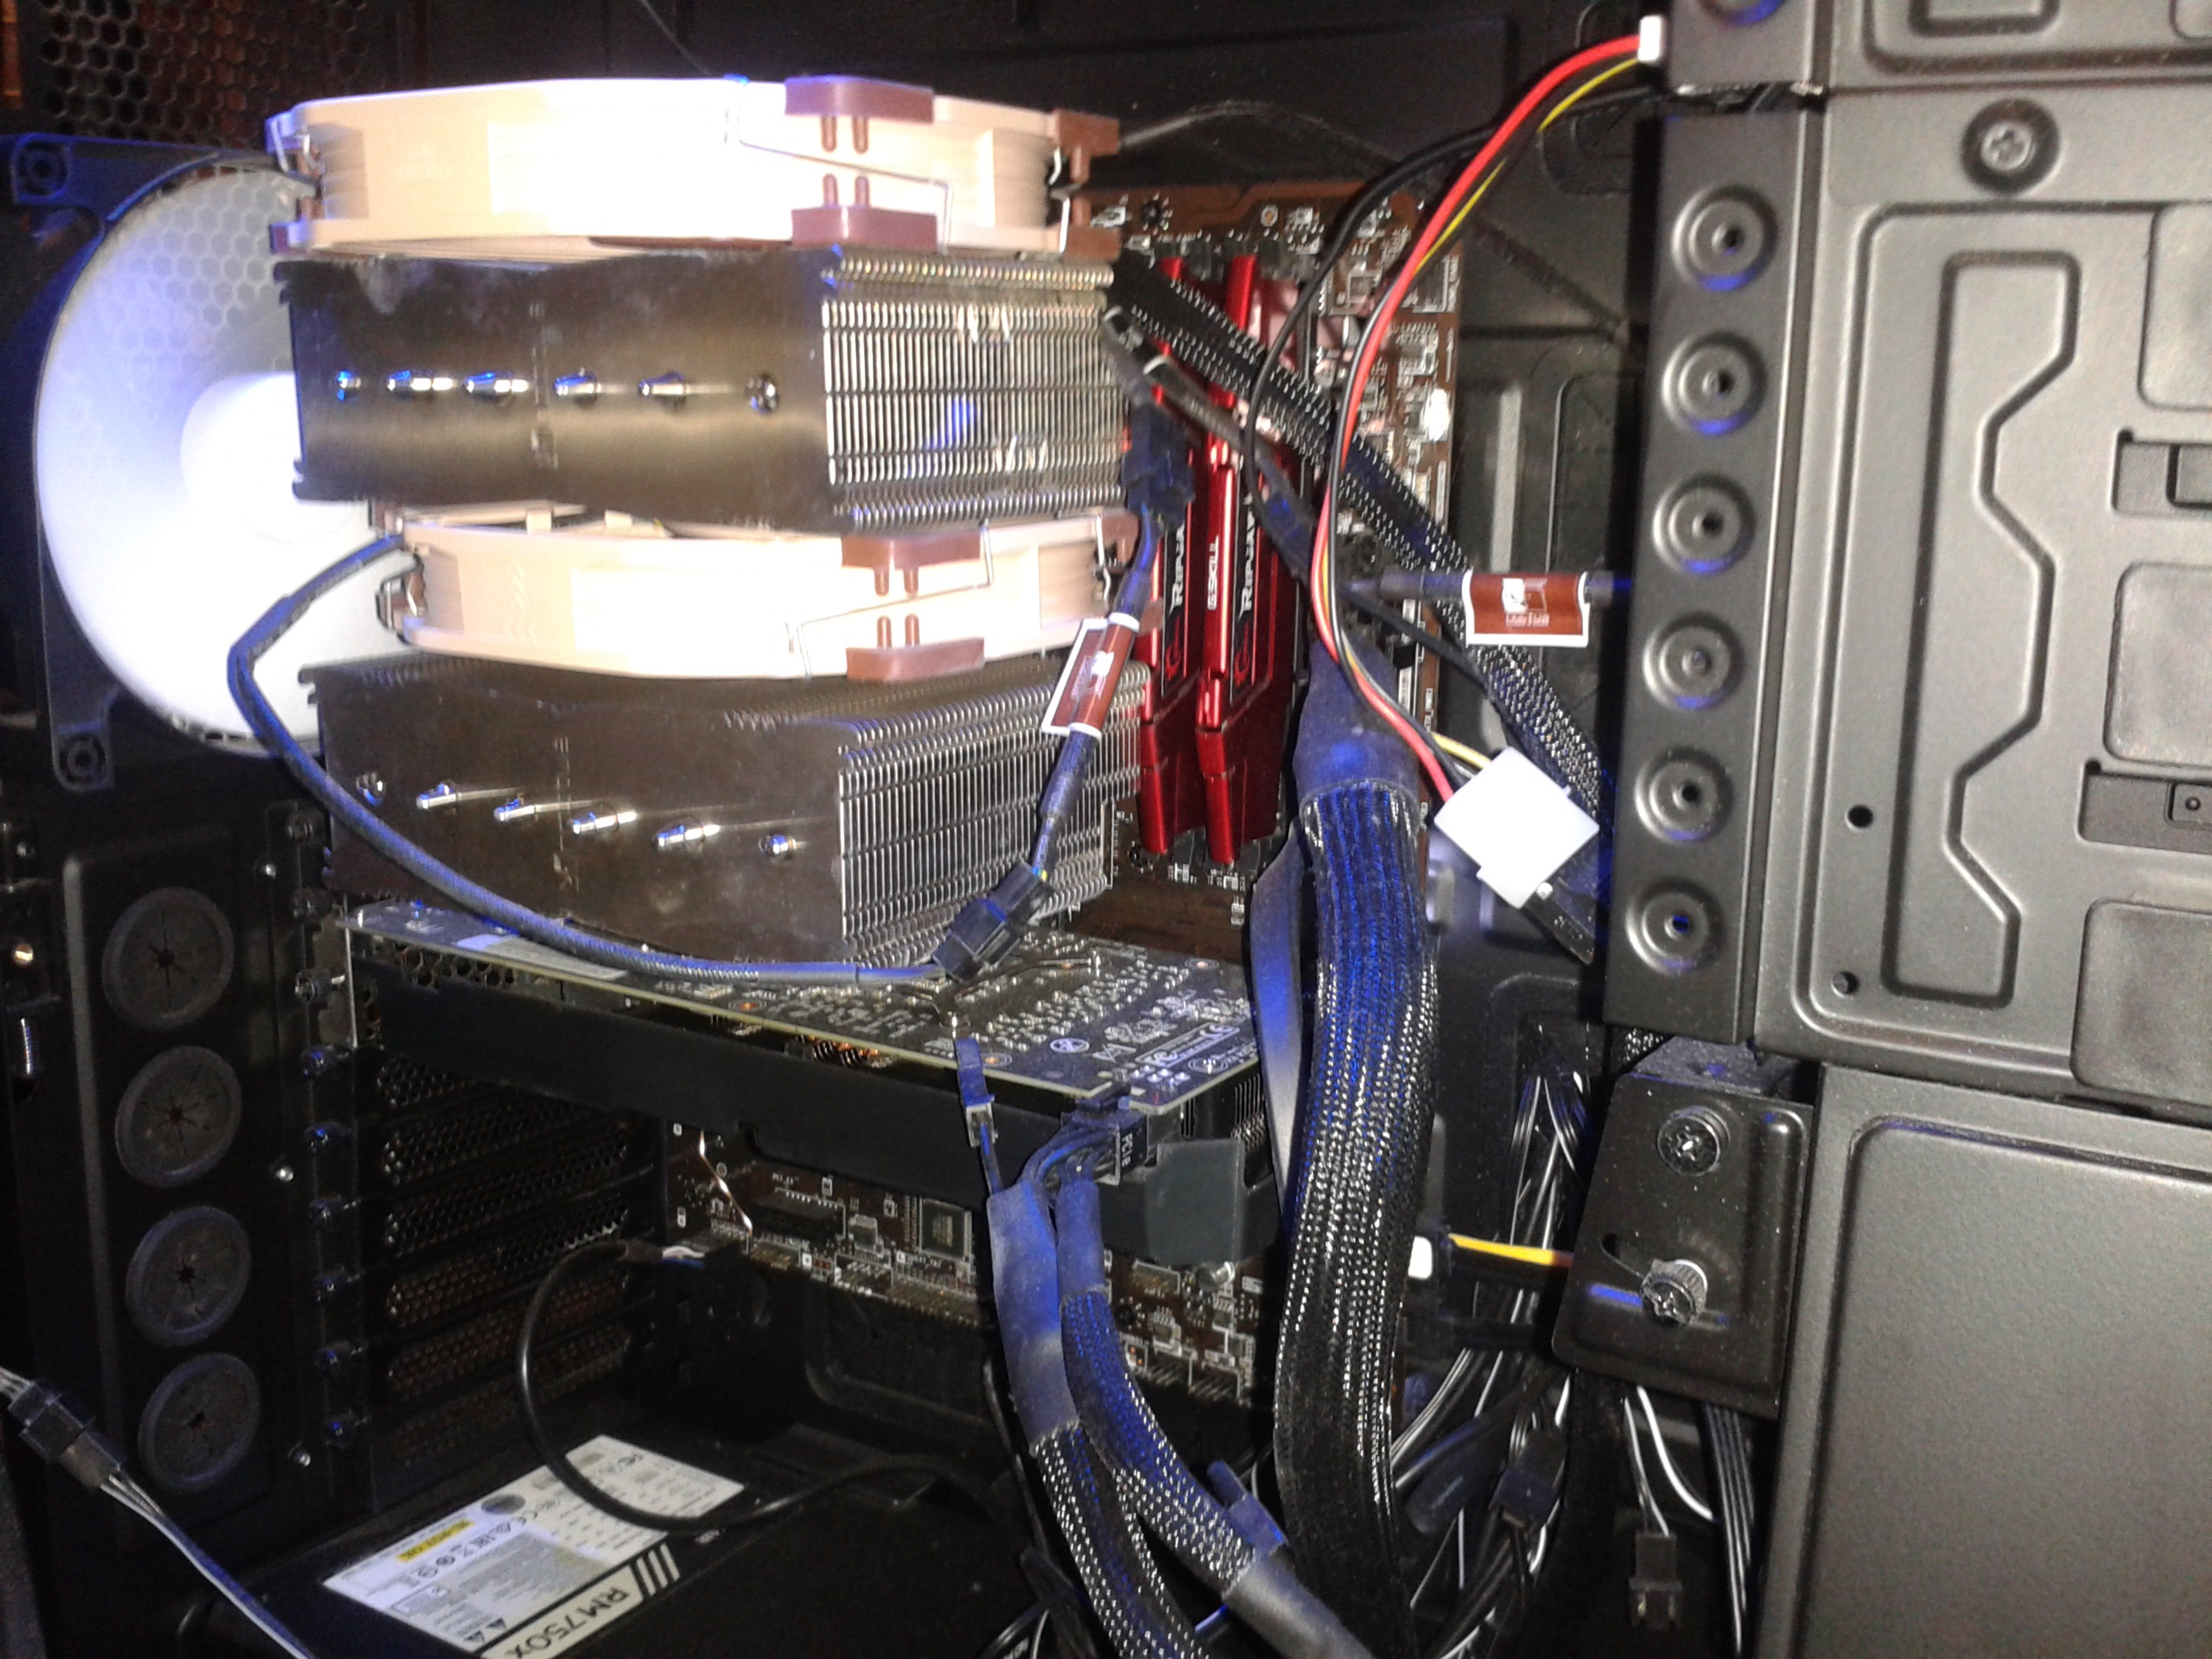
\includegraphics[height=0.6\textwidth]{chapter2/pictures/pc.pdf}
    		    \caption[Desktop PC]{Aufbau eines gewöhnlichen Desktop-Computers}
    		    \label{2:gpucpu}
		\end{figure}
		
		Datenverkehr zwischen CPU und GPU erfolgt meistens über \Gls{PCIe}x16 mit einer maximalen physikalischen Bandbreite von 32GB/s (25GB/s ohne Overhead). Sehr hochwertige Karten sind über \gls{nvlink} miteinander verbunden bei einer \Gls{Peak Bandwidth} von 300GB/s, was immer noch weit unter der internen Speicherbandbreite liegt. Kopieranweisungen zwischen CPU und GPU sollte also auf das Minimum reduziert werden.
		
		Nvidia bietet im Wesentlichen drei Produktlinien an:
		\begin{itemize}
		    \item \textbf{GeForce}: Gaming-Grafikkarten. Berechnungen für Gaming beschränken sich meist auf das Berechnen von Texturen und Ausgabe auf dem Bildschirm. Daher sind diese Karten nicht mit einem Rechenwerk für doppelte Präzision ausgestattet und verlieren einen erheblichen Faktor bei der Performance ($\approx 32$), sollte man 64Bit Arithmetik anwenden.
		    
		    \newpage
		
		    \item \textbf{Quadro}: Ausgestattet für HPC. Diese verlieren nur den Faktor zwei bei doppelter Präzision. Verwendet werden diese für CAD (Differentialgleichungen lösen und grafisch anzeigen für Belastungsanalysen) oder grafische Simulationen.
		    
		    \begin{center}
		    \includegraphics[width=0.8\textwidth]{chapter2/pictures/haken.pdf}
		    
		    \includegraphics[width=0.6\textwidth]{chapter2/pictures/mesh.pdf}
		    \end{center}

		    \item \textbf{Tesla} wie Quadro, aber ohne Video-Controller. Diese sind im Wesentlichen für Deep-Learning Techniken gedacht. Moderne GPUs beinhalten sogenannte Tensorkerne, die für \textit{deep-convolutional neural networks} optimiert sind. Diese kommen nun vermehrt in Gaming Karten als Unterstützung für Ray-Tracing Kerne zum Einsatz.
		\end{itemize}		 		
		
        Karten aller drei Linien werden nach ihrer Chiparchitektur klassifiziert. Von der ältesten zur modernsten heißen diese: Tesla (nicht verwechseln!), Fermi, Maxwell, Kepler, Pascal, Volta (Weiterentwicklung: Turing)
        
        Zudem existieren Unterkategorien, die in der sogenannten \textit{\gls{compute capability}} zum Ausdruck kommen. Diese ist die wesentlichste Kenngröße einer Nvidia Grafikkarte, da sie bestimmt, welche Features von CUDA in Hardware auf der GPU implementiert sind.		
		
		Eine GPU ist im Wesentlichen ein Verbund aus tausenden Kernen, sogenannten \Glspl{Thread}, mit relativ geringer Leistung. Nach dem SIMD Prinzip führen alle Kerne ähnliche Tätigkeiten aus. Die Idee hinter HPC auf GPUs ist, die massive Parallelität für Tätigkeiten auszunutzen, die bestimmte Eigenschaften erfüllen:
		\begin{itemize}
			\item Probleme mit extrem hoher Parallelität, z.B. sehr große unabhängige Schleifen.
			\item Probleme mit sehr vielen ähnlich gelagerten Berechnungen, also die selben Operationen in der gleichen Reihenfolge aber mit unterschiedlichen Daten.
			\item Probleme mit einer geringen \Gls{Arbeit} in jedem parallelen Prozess, z.B. einfache mathematische Formeln.
			\item Probleme mit geringem Speicherfluss.			
		\end{itemize}

		Eine GPU wird aufgeteilt in eine bestimmte Anzahl von sogenannten Streaming Multiprocessors (\Gls{SM}). Üblich ist eine geringe zweistellige Anzahl (Abb. \ref{2:gpu}). Diese bestehen wiederum aus den folgenden Komponenten:
		
		\begin{itemize}
	        	\item Multiple Threaded Instruction Unit (\Gls{MTIU}): verteilt die Instruktionen auf einen \Gls{Thread} pro \Gls{Warp}
        		\item \Glspl{Warp}: ein Verbund von 32 \Glspl{Thread}. Eine Instruktion wird kopiert und an alle weitergegeben.
		    \item \Gls{Halfwarp}: Genau eine Hälfte eines \glspl{Warp}
		    \item Special Function Unit (SFU): Erledigt besondere Aufgaben, z.B. shader Berechnungen (später mehr) 
        		\item \Gls{shared Memory}: ein kleiner, extrem schneller Speicher, den sich alle \Glspl{Thread} eines \Gls{SM}s teilen.
		\end{itemize}
		
		\begin{figure}[h]
			\centering
    	        \includegraphics[width=\textwidth]{chapter2/pictures/sm.pdf}
    	        \caption[GPU]{Aufbau einer GPU}
    		    \label{2:gpu}
		\end{figure}

		Es ist wichtig, die technischen Details der Hardware zu kennen, um die Software darauf anzupassen. Ein HPC Programm ist üblicherweise genau auf die Hardware zugeschnitten, auf der das Programm laufen soll. Die Generalisierung eines Problems ist nicht trivial und manchmal sogar unmöglich oder nur unter starken \Gls{Performance}verlusten zu erreichen.	
	\stopcontents[Hardwaregrundlagen]
	
	\startcontents[Einführung in Nvidia CUDA]
    \printcontents[Einführung in Nvidia CUDA]{l}{1}{\chapter*{Einführung in Nvidia CUDA}\setcounter{tocdepth}{2}}
		\chapter{Einf\"uhrung in Nvidia CUDA}
	Seit 2007 existiert das Nvidia Produkt \textit{Compute Unified Device Architecture} (CUDA). Dabei handelt es sich um eine Programmiersprache, eine Compilerarchitektur, eine Runtime-Library oder kurz gesagt um eine Platform. CUDA lässt sich mit dem \textit{Nvidia CUDA Toolkit} leicht auf Linux, MacOS oder Windows installieren und bringt dabei mehrere HPC Bibliotheken mit. Auf einige soll später noch eingegangen werden. Die wichtigsten Vertreter sind:
	\begin{itemize}
		\item \textbf{cuBLAS}:   Die CUDA Implementierung der \textit{Basic Linear Algebra Subprograms}.
		\item \textbf{curand}:   Ein Zufallszahlen-Generator (RNG) und verschiedene Verteilungen.
		\item \textbf{cuSOLVER}: Eine Implementierung der beliebtesten Matrixzerlegungen.
		\item \textbf{THRUST}:   Die CUDA Implementierung der C++ Standard Template Library (STL).
	\end{itemize}
	Andere prominente Vertreter sind cuDNN, TensorRT und offizielle Partnerprojekte wie MAGMA, GROMACS oder Tensorflow.
				
		
		\section{C Runtime}
		Ein Hauptprogramm auf der CPU wird üblicherweise in C oder C++ geschrieben. Wahlweise lässt sich auch ein \Gls{API} in einer anderen Programmiersprache benutzen, z.B. pyCUDA in Python. Dieses Programm läuft wie gewohnt auf der CPU und wird fortan als Hostcode bezeichnet. Eine sehr rechenintensive Stelle im  Hostcode soll nun auf die GPU ausgelagert werden. Im gleichen Quellcode wird nun in der Programmiersprache CUDA ein sogenanntes \Gls{Kernel} definiert.
			\subsection*{Kernels}
			\Glspl{Kernel} sind sehr kleine Recheneinheiten, die parallel auf der GPU ausgeführt werden sollen. Der folgende Code zeigt ein \Gls{Kernel} zur Addition zweier Vektoren.
	  		\begin{lstlisting}[caption=~Vektoraddition Kernel]
				__global__ void VecAdd(float* A, float* B, float* C, int N)
				{
    				int i = threadIdx.x;
    				if (i < N)
        				C[i] = A[i] + B[i];
				}
				
				...
				
				int main()
				{		
					...
					VecAdd<<<1, N>>>(A, B, C, N) ;
					...
				}
			\end{lstlisting}
			
			\Glspl{Kernel} werden immer mit dem Keyword \li`__global__` deklariert und der Rückgabetyp ist immer \li`void`. \Gls{Kernel}aufrufe erfolgen asynchron, d.h. die CPU schickt den Auftrag lediglich ab und arbeitet dann weiter den Hostcode ab. Mehrere \Gls{Kernel}aufrufe hintereinander werden auf der GPU serialisiert.
			
			Die spitzen Klammern geben an, mit welchen \Glspl{Thread} der Code ausgeführt werden soll. Im obigen Fall wird das \Gls{Kernel} mit $N$ \Glspl{Thread} gestartet. Ausnahmslos jeder dieser \Glspl{Thread} erhält das \Gls{Kernel} und führt den Code aus: Jeder \Gls{Thread} rechnet sich seinen Index aus (entspricht dem Prozessor-rank). Jeder \Gls{Thread} nimmt einen Wert von A und B, rechnet die Summe aus und schreibt genau einen Wert von C. Ein \Gls{Kernel} kann man sich also so vorstellen, als würde man eine Schleife ausrollen und jedes Element einzeln und parallel berechnen. \Glspl{Kernel} können nicht auf Hostcode zugreifen. Sollte $N$ größer sein als die Länge der Vektoren, so müssen die überzähligen \Glspl{Thread} warten. Ein Weglassen der if-Abfrage würde jedoch nicht zwingend zu einem Fehler führen. Um falsche Speicherzugriffe zu vermeiden, kann das Tool \li`cuda-memcheck` verwendet werden. (später mehr)
			
			Zur besseren Steuerung der \Glspl{Thread} teilt man diese in \Glspl{Block} ein\footnote{Meistens existieren technische Obergrenzen für die Zahl an Threads pro Block.}. Die Gesamtheit an \Glspl{Block}n bezeichnet man als \Gls{Grid}.
			
			\begin{lstlisting}[caption=~Kernelaufruf]		
				int main()
				{
					int threadsPerBlock = 32;
					int blocksPerGrid = N / threadsPerBlock;
					
					...
					
					VecAdd<<<blocksPerGrid, threadsPerBlock>>>(A, B, C, N);
					
					...					
				}
			\end{lstlisting}

			In diesem Beispiel übergibt man im ersten Element zwischen den spitzen Klammern die Zahl an \Glspl{Block}n und im zweiten die Zahl an \Glspl{Thread} pro \Gls{Block}. Beide Zahlen multipliziert ergeben also die Zahl an \Glspl{Thread} insgesamt. Mittels \li`blockIdx.x*blockDim.x + threadIdx.x` berechnet man den globalen Index eines \Glspl{Thread}. Die \Glspl{MTIU} verteilen die \Glspl{Block} dann automatisch auf die \Gls{SM}. Sollten mehr \Glspl{Thread} involviert werden als tatsächlich zur Verfügung stehen, so wird zuerst eine passende Anzahl verteilt und dann für die restlichen \Glspl{Block} wiederholt. Der Index zählt dabei korrekt weiter, da er von der ID des \Gls{Block}s abhängt.
			
			Falls das \Gls{Kernel} eine Funktion aufrufen soll, so muss diese extra für das Device geschrieben werden. Dazu deklariert man diese Funktionen mit dem Keyword \li`__device__`. Analog dazu werden gewöhnliche Funktionen auf der CPU mit \li`__host__` deklariert. Wird kein Keyword geschrieben, so handelt es sich um eine Host Funktion. Wird eine Funktion mit beidem deklariert, so wird die Funktion für Device und Host kompiliert. Device Funktionen können nicht vom Host gerufen werden und umgekehrt. Eine Device Funktion darf einen return Wert haben.
			
			\subsection*{C++ Kompatibilit\"at}
			Die Programmiersprache CUDA orientiert sich an C11. Es können alle Features dieses Standards benutzt werden. C++ Code als Device Code zu schreiben ist allerdings wesentlich schwieriger und wurde daher nur teilweise implementiert. Eine Liste der C++ Features enthält der CUDA Programming Guide in Anhang F. \autocite{cudaPG} 
			
			
		\section{Speichermodell}
		Eine GPU kennt mindestens fünf Arten von Speicher:
		\begin{itemize}
			\item \Gls{global Memory}: Daten, die vom CPU Speicher kopiert werden, werden in diesem gespeichert. Dieser Speicher ist ausnahmslos allen \Glspl{Thread} zugänglich.
			\item \Gls{constant Memory}: Ein ebenfalls globaler Speicher. Konstante Variablen werden so read-only abgespeichert und verhalten sich ähnlich den konstanten Variablen in C (Vermeidung von Bankkonflikten).
			\item \Gls{local Memory}: Jeder \Gls{Thread} verfügt über einen sehr kleinen Speicher für Hilfsvariablen, die nur diesem zugänglich sind. Definiert man eine Variable im Devicecode, so wandert sie in den lokalen Speicher (z.B. der Index \li`int i`). Dieser Speicher ist ähnlich langsam wie \gls{global Memory}, wird aber in einen Cache geladen.
			\item \Gls{shared Memory}: Ein kleiner, extrem schneller Speicher, den sich jeweils die \Glspl{Thread} einer \Gls{SM} teilen. Pro \Gls{SM} ist ein Element in der GPU integriert.
			\item \Gls{texture Memory}: Ein interpolierender, globaler Speicher, der für Texturen, also multidimensionale Speicherstrukturen optimiert wurde.
		\end{itemize}
		
		\newpage
		
		Um die Vektoraddition von oben durchzuführen, muss die CPU zunächst die Vektoren in den \Gls{global Memory} kopieren. Folgendes Beispiel illustriert dies:		
		\begin{lstlisting}[caption=~Vektoraddition Host]
			uint N = 256;
			uint size = N∗sizeof(float);
			float ∗h_A = (float ∗)malloc(size);
			float ∗h_B = (float ∗)malloc(size);
			float ∗h_C = (float ∗)malloc(size);

			float ∗d_A;
			cudaMalloc(&d_A, size);
			float ∗d_B;
			cudaMalloc(&d_B, size);
			float ∗d_C;
			cudaMalloc(&d_C, size);
			
			
			cudaMemcpy(d_A, h_A, size, cudaMemcpyHostToDevice);
			cudaMemcpy(d_B, h_B, size, cudaMemcpyHostToDevice);

			int threadsPerBlock = 32;
			int blocksPerGrid = N / threadsPerBlock ;
			VecAdd<<<blocksPerGrid, threadsPerBlock>>>(d_A, d_B, d_C, N);
			cudaMemcpy(h_C, d_C, size, cudaMemcpyDeviceToHost);
			
			cudaFree(d_A); cudaFree(d_B); cudaFree(d_C);
			free(h_A); free(h_B); free(h_C);
		\end{lstlisting}	
		
		Der Befehl \li`cudaMalloc` erstellt einen Buffer der entsprechenden Größe im \Gls{global Memory}.
		Der Befehl \li`CudaMemcpy` kopiert dann den Speicher des Hostvektors in den Devicevektor auf der Grafikkarte. Dabei gibt \li`size` die Anzahl an Bytes an, die kopiert werden soll. Für eine einzelne Variable ($N$) ist dies nicht notwendig.
		Nachdem das Kernel abgeschickt wurde, wird der Ergebnisvektor auf den Host zurückkopiert. Auf die Pointervariablen lässt sich mittels Pointeraddition ein Offset angeben, die Größe muss aber entsprechend angepasst werden. Beispielhaft kopiert \li`(d_A+3, h_A+5, 20, ...)` exakt 20 Bytes beginnend von \li`h_A[5]` nach \li`d_A[3]`.
		Hinter \li`cudaMemcpy` verbirgt sich ein impliziter \Gls{Kernel}aufruf, der synchron abläuft, d.h. die CPU muss warten bis das \Gls{Kernel} ausgeführt wurde. Es ist zu beachten, dass \Gls{Kernel}aufrufe normalerweise asynchron laufen, also die CPU nicht blockieren (non-blocking). 
		Speicher auf dem Device wird mit \li`cudaFree` freigegeben.
		
		\Gls{shared Memory} wird mit dem Keyword \li`__shared__` deklariert. Der erste \Gls{Thread}, der in einem \Gls{Kernel} auf eine solche Instruktion trifft, legt eine Variable im \gls{shared Memory} der entsprechenden Größe an. Diese Variable teilen sich dann alle \Glspl{Thread} eines \Gls{Block}s. Existieren insgesamt $n$ \Glspl{Block}, so existieren auch $n$ verschiedene Variablen. In der statischen Variante muss die Größe des Arrays zur Compile-Zeit bekannt sein.
		\begin{lstlisting}[caption=~shared Memory statisch]
			__global__ void test()
			{
  				__shared__ int s[64];
  				...
			}
  		\end{lstlisting}

		Im Gegensatz zur statischen Variante lässt sich \gls{shared Memory} auch dynamisch allozieren:  		
  		\begin{lstlisting}[caption=~shared Memory dynamisch]
			__global__ void test()
			{
  				extern __shared__ int s[];
  				...
			}
			
			int main()
			{
				...
				int shared_memory_size = ...
				test<<<1, threadsPerBlock, shared_memory_size>>>();
				...
			}			
  		\end{lstlisting}
  		
        Dem \Gls{Kernel} muss die Größe des \gls{shared Memory} (pro \Gls{Block}) mitgegeben werden. In beiden Fällen wird also die Allozierung des Speichers von der CPU übernommen.  Dynamische Speicherverwaltung ist mittlerweile auch auf dem Device möglich. Darauf wird jedoch erst später eingegangen (siehe Abschnitt \ref{conc}). 
        
        Sollen mehrere Arrays im \gls{shared Memory} abgelegt werden, so definiert man sich lediglich Pointer auf ein großes Gesamtarray. Der Beginn des jeweils neuen Arrays sollte sinnvollerweise dem Ende des vorangegangenen entsprechen.  	  		
  		\begin{lstlisting}	[caption=~shared Memory verteilt]	
			extern __shared__ int s[];
			int *integerData = s;                        
			float *floatData = (float*)&integerData[nI];
			char *charData = (char*)&floatData[nF];
			
			...
			
			test<<<1, threadsPerBlock, 
				nI*sizeof(int) + nF*sizeof(float) + nC*sizeof(char)>>>(...);
		\end{lstlisting}

		Im folgenden Beispiel wird die Vektoraddition umgeschrieben, um sich die Vektoren A und B in den \gls{shared Memory} zu laden:	
		
		\begin{lstlisting}[caption=~Vektoraddition shared Memory]
			__global__ void VecAdd(float* A, float* B, float* C, int N)
			{
    			int i = blockDim.x * blockIdx.x + threadIdx.x;
    			int tid = threadIdx.x;
    			
    			__shared__ float As[blockDim.x];
    			__shared__ float Bs[blockDim.x];
    			
    			if (i < N)
    			{
    			    As[tid] = A[i];
    			    Bs[tid] = B[i];
    			    
    			    ...
    			    
        			C[i] = As[tid] + B[tid];
        		}
			}
		\end{lstlisting}
		
		Da ohnehin einmal \li`A[i]` und \li`B[i]` aus dem Speicher geladen werden müssen, ist es hier unsinnig, den Speicher überflüssigerweise zu kopieren. Allerdings könnten ja vor der Addition \li`As` und \li`Bs` noch mehrmals gebraucht werden. Die Aufgabe des Programmierers ist es nun herauszufinden, bei welcher Datengröße abhängig vom Algorithmus der \Gls{Performance}gewinn durch die höhere Bandbreite den Verlust durch das Kopieren übersteigt.
		
		\Gls{constant Memory} wird mit dem Keyword \li`__constant__` als globale Variable deklariert. Mit dem Befehl \li`cudaMemcpyToSymbol` wird diese dann in den Speicher der GPU kopiert und steht dort dann auch global zur Verfügung, muss also beim \Gls{Kernel}aufruf nicht explizit angegeben werden:
		\begin{lstlisting}[caption=~Vektoraddition constant Memory]
			__constant__ float d_A[12800];
			__global__ void VecAdd(float* B, float* C, int N)
			{
    			int i = blockDim.x * blockIdx.x + threadIdx.x;
    			if (i < N)
        			C[i] = d_A[i] + B[i];
			}
			
			...
			
			cudaMemcpyToSymbol(d_A, h_A, size);
			VecAdd<<<blocksPerGrid, threadsPerBlock>>>(d_B, d_C, N);
		\end{lstlisting}
		
		Der \gls{constant Memory} ist ebenfalls ein globaler Speicher und steht jedem \Gls{Thread} zur Verfügung. Allerdings müssen Aufrufe der selben Stelle im Speicher zur selben Zeit innerhalb eines \Glspl{Warp} (Bankkonflikt) nicht serialisiert werden. Daher eignet sich dieser Speicher besonders für konstante Skalare, z.B. Naturkonstanten.
		
		\section{Mehrdimensionale Bl\"ocke}
		Bisher wurden \Gls{Kernel} immer nur mit eindimensionalen \Glspl{Block}n und \Glspl{Grid} ausgeführt. Allerdings verbirgt sich dahinter ein Typecast. Zum Beispiel wird \li`<<<1,N>>>` zu \li`<<<dim3(1,1,1), dim3(N,1,1)>>>`. \li`dim3` bezeichnet dabei eine eingebaute Datenstruktur, die aus drei vorzeichenlosen Ganzzahlen besteht. In diesem Fall gibt sie die Anzahl der \Glspl{Block} im \Gls{Grid} bzw. der \Glspl{Thread} pro \Gls{Block} in die Raumrichtungen \li`(x,y,z)` an. Das \Gls{Grid} und die \Glspl{Block} sind also keine Ketten sondern Quader von Objekten. Die Indizes der \Glspl{Block} und \Glspl{Thread} lassen sich dann Spalten-, Zeilen- und Ebenenweise abfragen: 			
		\begin{lstlisting}[caption=~Multidimensionale Blöcke]
			__global__ test()
			{
				int row = blockIdx.y * blockDim.y + threadIdx.y;
				int col = blockIdx.x * blockDim.x + threadIdx.x;
				...
			}
    		
    		...

		    dim3 dimBlock(BLOCK_SIZE, BLOCK_SIZE);
    		dim3 dimGrid(GRID_SIZE, GRID_SIZE;
    		test<<<dimGrid, dimBlock>>>();
		\end{lstlisting}
        In diesem Fall werden also \Glspl{Block} der Größe \li`BLOCK_SIZE`$\times$\li`BLOCK_SIZE` in einem \Gls{Grid} mit \li`GRID_SIZE`$\times$\li`GRID_SIZE` \Glspl{Block}n angeordnet. Bei modernen GPUs ist die Obergrenze für die Dimension der \Glspl{Block} \li`(1024,1024,64)`.
        
        Das folgende Beispiel behandelt die Matrixmultiplikation unter Zuhilfenahme von \gls{shared Memory} und Multidimensionalen \Glspl{Block}n:       
        \begin{lstlisting}[caption=~Matrixmultiplikation]
			#define BLOCK_SIZE 16 	
			typedef struct
			{
				uint width;
				uint height;
				float* elements;
				uint stride;
			} Matrix;

			__device__ 
			float GetElement(const Matrix A, uint row, uint col)
			{
				return A.elements[row * A.stride + col];
			}

			__device__ 
			void SetElement(Matrix A, uint row, uint col, float value)
			{
				A.elements[row * A.stride + col] = value;
			}
			
			__device__
			Matrix GetSubMatrix(Matrix A, uint row, uint col) 
			{
				Matrix Asub;
				Asub.width    = BLOCK_SIZE;
				Asub.height   = BLOCK_SIZE;
				Asub.stride   = A.stride;
				Asub.elements = &A.elements[A.stride * BLOCK_SIZE * row 
					+ BLOCK_SIZE * col];
				return Asub;
			}	
			 
			__global__ 
			void MatMulKernelShared(const Matrix A, const Matrix B, Matrix C)
			{    
    			uint blockRow = blockIdx.y;
    			uint blockCol = blockIdx.x;

    			Matrix Csub = GetSubMatrix(C, blockRow, blockCol);
    
    			float Cvalue = 0;

    			uint row = threadIdx.y;
    			uint col = threadIdx.x;

    			for (uint m = 0; m < (A.width / BLOCK_SIZE); ++m)
    			{
					Matrix Asub = GetSubMatrix(A, blockRow, m);
					Matrix Bsub = GetSubMatrix(B, m, blockCol);

					__shared__ float As[BLOCK_SIZE][BLOCK_SIZE];
					__shared__ float Bs[BLOCK_SIZE][BLOCK_SIZE];
					As[row][col] = GetElement(Asub, row, col);
					Bs[row][col] = GetElement(Bsub, row, col);

					__syncthreads();

					for (uint e = 0; e < BLOCK_SIZE; ++e)
							Cvalue += As[row][e] * Bs[e][col];

					__syncthreads();
				}

				SetElement(Csub, row, col, Cvalue);
			}
        \end{lstlisting}
        
        Abbildung \ref{fig3:matmul} zeigt klar, dass \gls{shared Memory} die bessere Alternative zu einer naiven Implementierung ist. Die Funktion \li`__syncthreads()` wird in Abschnitt \ref{sync} besprochen.
        
        \begin{figure}[h]
  		\centering
  		\scalebox{1.3}{
  		\begin{tikzpicture}
    		\begin{axis}[/pgf/number format/.cd, use comma, 1000 sep={}, xlabel={dimension $n$}, ylabel={computation time / sec.}, legend pos=outer north east, legend style={cells={align=left}}]
      		\addplot [draw=UR@color@12!50!black, mark=*, only marks, mark options={scale=.5}, fill=UR@color@12!50!white]   table[x index=0, y index=1]{/home/kat10110/script/chapter3/plots/matmul.dat};
      		\addlegendentry{ohne shared memory}
      		\addplot [draw=gray!50!black, mark=*, only marks, mark options={scale=.5}, fill=gray!50!white] table[x index=0, y index=2]{/home/kat10110/script/chapter3/plots/matmul.dat};
      		\addlegendentry{mit shared memory}     
    		\end{axis}
    	\end{tikzpicture}}
  		\caption[Matrixmultiplikation shared Memory]{Laufzeitvergleich von Matrixmultiplikationen der Größ e $n\times n$ mit und ohne shared Memory. Zum Einsatz kam eine \textit{Nvidia GTX 1060}.}
  		\label{fig3:matmul}
		\end{figure}
        
        Dieser Algorithmus ist nicht ohne Weiteres anwendbar, falls sich die Matrizen nicht bequem auf gleich große \Glspl{Block} verteilen lassen.
        
        Aus den genannten Beispielen ergeben sich Merkregeln für die Wahl der \Gls{Thread}zahl pro \Gls{Block}:
        \begin{itemize}
        	\item Die Anzahl sollte ein Vielfaches von 32 sein, um unregelmäßiges Arbeiten der \Glspl{Warp} zu verhindern.
        	\item Die Anzahl sollte ein Vielfaches der Anzahl von \Glspl{Thread} pro \Gls{SM} sein, um unregelmäßiges Mapping von physischem Speicher in den selben Adressraum zu verhindern.
        	\item Die Anzahl sollte so gewählt sein, dass sich die gesamte Problemgröße, also ein oder mehrere \Glspl{Grid}, exakt auf gleich große \Glspl{Block} verteilen lässt.
        	\item Die Gesamtzahl der \Glspl{Thread} im \Gls{Grid} sollte ein Vielfaches der insgesamt in Hardware zur Verfügung stehenden \Glspl{Thread} sein, um die GPU voll auszulasten.
        \end{itemize}
        
        Da in der Praxis diese Punkte kaum alle einzuhalten sind, ist ein Blackbox-Verfahren für die GPU schwer oder gar nicht zu programmieren. Lässt sich die Zahl der Werte $N$ nicht bequem auf \Glspl{Block} und \Glspl{Thread} verteilen, so muss \li`N / threadsPerBlock` auf die nächst größere Zahl aufgerundet werden. Dazu berechnet man mit einer Integerdivision \li`blocksPerGrid = (N + threadsPerBlock - 1) / threadsPerBlock`. Wenn möglich sollte man bereits bei der Erzeugung von Messdaten in einem Experiment oder in einer Simulation auf vernünftige Problemgrößen achten, andernfalls muss man mit \Gls{Performance}einbußen rechnen.
        								
		\section{Error Handling}
		Beinahe jeder \Gls{API}-Call liefert einen speziellen CUDA-Datentyp namens \li`cudaError_t`. Folgende Funktion fragt diesen Wert ab und gibt einen Fehlerstring zurück:		
		\begin{lstlisting}[caption=~Error Handling]
			#define CUDA_ERROR_CHECK

			#define CudaCheckError()  __cudaCheckError(__FILE__, __LINE__)

			inline void __cudaCheckError(const char *file, const int line)
			{
			#ifdef CUDA_ERROR_CHECK
				cudaError err = cudaGetLastError();
				if(cudaSuccess != err)
				{
					fprintf(stderr, "cudaCheckError() failed at %s:%i : %s\n",
					file, line, cudaGetErrorString(err));
					exit(-1);
				}

    			err = cudaDeviceSynchronize();
    			if(cudaSuccess != err)
    			{
        			fprintf(stderr, "cudaCheckError() with sync failed at 
        				%s:%i : %s\n",
					file, line, cudaGetErrorString(err));
					exit(-1);
				}
			#endif

				return;
			}
		\end{lstlisting}
		
		Diese Funktion wurde nicht im \Gls{API} implementiert, da das Errorhandling vom Design des gesamten Programms abhängt und daher dem Programmierer überlassen werden sollte. Funktionen dieser Art kursieren in mehreren Varianten in Foren und verschiedenen Handbüchern. Mittels \li`cudaGetLastError` wird der letzte Fehler untersucht. Da \Glspl{Kernel} asynchron laufen, kann es nötig sein, mittels \li`cudaDeviceSynchronize` zu synchronisieren, d.h. alle \Glspl{Kernel} müssen ausgeführt worden sein, bevor die CPU weiter Code ausführen darf (siehe Abschnitt \ref{sync}). Falls dies nicht nötig ist, sollte die Zeile kommentiert werden. Um Rechenzeit zu sparen, kann durch das \li`CUDA_ERROR_CHECK` Makro diese Funktion zur Compile-Zeit entfernt werden. CUDA Librarys (z.B. cuDNN oder cuRAND) definieren oft neue Datentypen für Fehler. Diese Funktion kann also in mehreren Variationen nötig sein.


		\section{Stream Processing}
		\subsection{Events}
        Um die Laufzeit zu messen, eignen sich CUDA-Events:		
		\begin{lstlisting}[caption=~Events]
			cudaEvent_t start, stop;
			cudaEventCreate(&start);
			cudaEventCreate(&stop);

			cudaEventRecord(start, 0);
			//zu messender Code//
			cudaEventRecord(stop, 0);	
		
			cudaEventSynchronize(stop);
			float milliseconds = 0;
			cudaEventElapsedTime(&milliseconds, start, stop);
		
			cudaEventDestroy(start);
			cudaEventDestroy(stop);
		\end{lstlisting}

		Mit \li`cudaEventRecord` werden zwei Events aufgezeichnet. Die Null am Ende teilt die Events dem Stream mit Nummer 0 zu (siehe \ref{streams}). Wird diese Angabe unterdrückt, so werden die Aufrufe automatisch diesem \Gls{Stream} zugeordnet (default-\Gls{Stream}). Nach dem Aufruf \li`cudaEventSynchronize`, also sobald das Event \li`stop` stattgefunden hat, kann mittels \li`cudaEventElapsedTime` die vergangene Zeit zwischen \li`start` und \li`stop` in Millisekunden gemessen werden.
		
		Zudem existiert \li`cudaError_t cudaEventQuery(cudaEvent_t event)`. Diese Funktion liefert dann einen Erfolg, falls das betreffende Event stattgefunden hat.
		
		Außerdem lassen sich mittels \li`cudaError_t cudaEventCreateWithFlags(cudaEvent_t* event, unsigned int flags)` Events mit Flags definieren, die sich in der Dokumentation der CUDA Runtime \Gls{API} nachlesen lassen. \autocite{cudaRTAPI}
		
      
		\subsection{Device Auswahl}
		Mittels \li`cudaGetDeviceCount` lässt sich ermitteln, über wie viele CUDA-fähige Grafikkarten die Platine, auf der die CPU sitzt, verfügt. Für jedes Gerät einzeln können dann die Eigenschaften des Geräts abgefragt werden.
		
		Die Geräte lassen sich mit \li`cudaSetDevice` manuell umschalten. Speicher der einen GPU lässt sich nur dann von der anderen abrufen, wenn der Peer-to-Peer Access mit \li`cudaDeviceEnablePeerAccess` aktiviert und der Speicher explizit zwischen den GPUs kopiert wird. Die Null am Ende teilt die Events dem Stream mit der Nummer 0 zu (siehe \ref{streams}). Wird diese Angabe unterdrückt, so werden die Aufrufe automatisch diesem \Gls{Stream} zugeordnet (default-\Gls{Stream}).
		\begin{lstlisting}[caption=~Device Peer-to-Peer Access]
			int deviceCount;
			cudaGetDeviceCount(&deviceCount);

			cudaDeviceProp deviceProp;
			cudaGetDeviceProperties(&deviceProp, 0);
			printf("Device %d has compute capability %d.%d.\n",
    			device, deviceProp.major, deviceProp.minor);
           
			cudaSetDevice(0);
			float* p0;
			cudaMalloc(&p0, size);
			test<<<...>>>(p0);
			
			cudaSetDevice(1);
			float* p1;
			cudaMalloc(&p1, size);
			test<<<...>>>(p1);
			
			
			
			cudaDeviceEnablePeerAccess(0, 0);
			test<<<...>>>(p0);
			
			cudaMemcpyPeer(p1, 1, p0, 0, size);
		\end{lstlisting}

	
		\subsection{Streams}\label{streams}
		Eine Menge von Instruktionen, die der Reihe nach abgearbeitet werden sollen, heißt \Gls{Stream}. Jene \Glspl{Stream} lassen sich beliebig erstellen und zerstören (\li`cudaStreamCreate`, \li`cudaStreamDestroy`). In folgendem Beispiel wird dynamisch eine Zahl von \Glspl{Stream} erstellt. Dann wird ein entsprechender Teil eines Gesamtarrays kopiert und ein Kernel ausgeführt. Damit dies in Reihe geschieht, werden sowohl \Gls{API}-calls als auch \Gls{Kernel} einem \Gls{Stream} zugeordnet.	
		
		\newpage
		
		\begin{lstlisting}[caption=~Streams]
			uint stream_num = ...;
			uint size = ...;	    
			float* hostPtr;
			cudaMallocHost(&hostPtr, stream_num * size);	
			//inputDevPtr allozieren und kopieren//
			cudaStream_t stream[stream_num];
			for (int i = 0; i < stream_num; ++i)
			{
				cudaStreamCreate(&stream[i]);
    			
				cudaMemcpyAsync(inputDevPtr + i * size, hostPtr + i * size,
					size, cudaMemcpyHostToDevice, stream[i]);
    			
				MyKernel <<<100, 512, 0, stream[i]>>>
					(outputDevPtr + i * size, inputDevPtr + i * size, size);
				
				cudaMemcpyAsync(hostPtr + i * size, outputDevPtr + i * size,
					size, cudaMemcpyDeviceToHost, stream[i]);
								
				cudaStreamDestroy(stream[i]);
			}
		\end{lstlisting}

		Die Idee dahinter ist, die CPU möglichst wenig zu blockieren (Asynchronizität) und möglichst viele \Gls{Kernel} gleichzeitig auszuführen (Concurrency). Allerdings bietet nicht jede GPU  Da ein normaler Kopierbefehl automatisch synchronisiert, muss die Kopie asynchron erfolgen (\li`cudaMemcpyAsync`). Mittels \li`cudaMallocHost` wird dafür sog. \gls{page-locked Memory} alloziert. Dieser Speicher darf vom Betriebssystem nicht verschoben werden und kann daher immer unter der selben Speicheradresse gefunden werden.
		
		Wird kein \Gls{Stream} angegeben, so wird der default-\Gls{Stream} verwendet. Für den default-Stream ist jede Form der Gleichzeitigkeit deaktiviert.
		
		Um die CPU auf einen bestimmten \Gls{Stream} warten zu lassen, kann \li`cudaStreamSynchronize` verwendet werden. \li`cudaStreamQuery` liefert genau dann einen Erfolg, wenn der \Gls{Stream} erfolgreich beendet worden.	
		
		\li`cudaStreamWaitEvent` beginnt mit der Ausführung eines \Glspl{Stream} erst, sobald ein bestimmtes Event aufgezeichnet wurde. Dieses Event kann ebenfalls einem \Gls{Stream} zugeordnet werden (\li`cudaEventRecord(start, stream[i])`).
		
		So lassen sich z.B. Abfragen erstellen,
		
		\li`if((cudaStreamQuery(stream[i]) == cudaSuccess) && (cudaEventQuery(stop) == cudaSuccess))...`
		
		mit denen man in Kombination mit der Device-Auswahl ganze Bäume von \Gls{Kernel}aufrufen erstellen kann. Auf Clustern kann man sich dies zu Nutze machen, um exakt den zeitlichen Ablauf von \Glspl{Kernel}s zu steuern.
		
		\textcolor{red}{Wichtig:}
		
		Funktionen, die dem default-\Gls{Stream} zugeordnet werden, haben bezüglich Synchronizität auf der GPU ein anderes Verhalten. Es gilt, dass alle \Gls{API} Aufrufe und \Glspl{Kernel} in ihrer Reihenfolge auf dem Device abgehandelt werden. Für eigene \Glspl{Stream} ist dies nicht zwingend der Fall (siehe Abschnitt \ref{async}).
		
		\subsection{Synchronisation}\label{sync}
		Explizite Synchronisierungsfunktionen:
		
		\begin{lstlisting}[caption=~Explizite Synchronisierung]
			__host__ cudaError_t cudaDeviceSynchronize(void)
			__host__ cudaError_t cudaStreamSynchronize(cudaStream_t)
			__host__ cudaError_t cudaEventSynchronize(cudaEvent_t)	
			__device__ void __syncthreads()
			__device__ void __syncwarp()
		\end{lstlisting}
		Erstere bildet für die CPU eine Barriere, bis sämtliche Kernels abgearbeitet wurden.
		
		Implizite Synchronisierung:
		\begin{itemize}
        	\item page-locked Host Memory Allozierung
			\item Device Memory Allozierung
			\item Setzen von Device Memory 
			\item Kopie zwischen zwei Adressen innerhalb desselben Device Memory
			\item ein beliebiges CUDA Kommando den 0-\Gls{Stream} betreffend,
			\item ein Wechsel zwischen L1/\gls{shared Memory} Konfigurationen beschrieben in \gls{compute capability} 3.x und \gls{compute capability} 7.x
		\end{itemize}
		
		\begin{figure}[h]
  		\centering
  		\scalebox{1.5}{
  		\begin{tikzpicture}
    		\begin{axis}[xlabel={dimension $n$}, ylabel={computation time / msec.}]
      		\addplot [draw=UR@color@12, mark=*, only marks, mark options={scale=.2}, fill=UR@color@12]   table[x index=0, y index=1]{/home/kat10110/script/chapter3/plots/prec.dat} node [below]{half};
      		%
      		\addplot [draw=gray!70!white, mark=*, only marks, mark options={scale=.2}, fill=gray!70!white] table[x index=0, y index=2]{/home/kat10110/script/chapter3/plots/prec.dat} node [left]{single~~~~~};
      		%
      		\addplot [draw=UR@color@12!50!black, mark=*, only marks, mark options={scale=.2}, fill=UR@color@12!50!black] table[x index=0, y index=3]{/home/kat10110/script/chapter3/plots/prec.dat} node [left]{double~~~~};    
    		\end{axis}
    	\end{tikzpicture}}
  		\caption[Axpy mit verschiedenen Präzisionen]{Laufzeitvergleich von Axpy-Operation ($\vec{y}\rightarrow a\cdot\vec{x}+\vec{y}$) der Grö\ss e $n$ mit half, single- und double-Präzision. Zum Einsatz kam eine \textit{Nvidia GTX 1060}.}
  		\label{fig3:axpy}
		\end{figure}
		
		
		\subsection*{\textcolor{red}{Divergenz}}
		Synchronisation ist nich nur aufgrund von Abhängigkeiten in Algorithmen notwendig. \Glspl{Thread} innerhalb eines \Glspl{Warp} müssen zur selben Zeit die selben Instruktionen erhalten. Ist dies im Programm nicht der Fall, z.B. durch if-else Verzweigungen, müssen diese Anweisungen serialisiert werden. Führen innerhalb eines jeden \Glspl{Warp} die \Glspl{Thread} paarweise unterschiedliche Instruktionen aus, so verliert man den Faktor 32 in der \Gls{Performance}. Diese sogenannte Divergenz kann nach jeder if-Anweisung oder abgebrochener Schleife auftreten und sollte so schnell wie möglich durch Synchronisierung aufgelöst werden. 
		
		
		\section{Datentypen}
		Auf GPUs existiert ein 16 Bit Datentyp mit halber Präzision. Benutzt man die in CUDA eingebauten arithmetischen Funktionen, kann man die Performance dadurch weiter verbessern.			
		\begin{lstlisting}[caption=~Half Precision]
		#include<cuda_fp16.h>
		#include "fp16_conversion.h"
		
		__global__
		void haxpy(int n, half a, const half *x, half *y)
		{
    		int start = threadIdx.x + blockDim.x * blockIdx.x;
    		int stride = blockDim.x;

			int n2 = n/2;
			half2 *x2 = (half2*)x, *y2 = (half2*)y;

			for (int i = start; i < n2; i+= stride) 
					y2[i] = __hfma2(__halves2half2(a, a), x2[i], y2[i]);

			if (start == 0 && (n%2))
					y[n-1] = __hfma(a, x[n-1], y[n-1]);
		}
		\end{lstlisting}
		
	    Die benutzten Funktionen verlangen den Datentyp \li`half2`, also eine Kombination von zwei \li`half` Werten.
	    
		Eingebaute Funktionen wären z.B. \li`__hdiv`, \li`__hadd` oder \li`__hmul`. Eine Auflistung aller Funktionen befindet sich in Kapitel 1.1 der Dokumentation der CUDA Math \Gls{API}. \autocite{cudaMath}
		
		Der Header \textit{cuda\_ fp16.h} befindet sich im üblichen include-Ordner. \textit{fp16\_ conversion.h} benötigt man jedoch aus dem github: \url{https://github.com/NVIDIA-developer-blog/code-samples/blob/master/posts/mixed-precision/fp16_conversion.h}
		
		Diese Datei enthält Konvertierungsfunktionen für \li`float` nach \li`half`.
	
		
		\section{Atomic Operations und Reduktionen}
		Eine Reduktion ist eine Operation, die die Dimensionalität eines Objekts verringert. Üblicherweise sind damit Operationen gemeint, die ein Array beliebiger Größe auf ein einfaches Skalar verringern. Beispiele dafür sind die Maximumsreduktion (also das Auffinden des größten Wertes), die Minimumsreduktion, die Summenreduktion (also die Summe aller Elemente) oder das Produkt aller Elemente. 
		
		Dies impliziert, dass viele \Glspl{Thread} gleichzeitig den selben Wert aktualisieren müssen, z.B. beim Addieren einer Zahl zu einem globalen Zähler. An dieser Stelle tritt ein sogenanntes Datarace auf: Ein \Gls{Thread} liest einen Wert aus dem Speicher, addiert und legt die Variable wieder im Speicher ab und überschreibt damit einen Wert der währenddessen von anderen \Glspl{Thread} bereits bearbeitet wurde bzw. bearbeitet wird. Um diese Zugriffe zu serialisieren, stellt CUDA sogenannte Atomic Operations zur Verfügung, also Operationen, die garantiert seriell ablaufen. Beispielsweise \li`int atomicAdd(int* address, int val)` addiert auf eine Variable bei der Speicheradresse \li`address` den Wert \li`val`. Eine Liste befindet sich im Anhang B.12 des CUDA Programming Guides. \autocite{cudaPG}
		
		Diese Form der Implementierung ist sehr langsam und eher zum Debuggen gedacht. Eine parallele Methode ist erforderlich. Im Prinzip nimmt zu Beginn jeder \Gls{Thread} zwei Werte und führt die Operation aus. Der nächste \Gls{Thread} nimmt abermals zwei Werte ohne Überlapp zum Vorherigen. Nach einem Schritt hat sich die Anzahl der zu reduzierenden Elemente halbiert. Im nächsten Schritt wird mit der halben Zahl der \Glspl{Thread} abermals halbiert, bis die Reduktion bereit steht.
		
		Im Folgenden wird eine naive Implementierung mit einfachen Mitteln optimiert.
		
		--SIEHE reduction.cu--
		
		Verschiedene HPC Librarys bieten Implementierungen der gängigsten Reduktionen an, z.B. THRUST oder MAGMA. 
		
		
		\section{NVCC}
		Der Nvidia CUDA Compiler (\gls{nvcc}) wird benutzt um sowohl Host- als auch Devicecode zu kompilieren. Es handelt sich dabei um eine Obermenge des g++. Es lässt sich bis zum C++14 Standard alles in C oder C++ kompilieren. Soll explizit CUDA Code kompiliert werden, so muss die Quelldatei die Dateiendung \li`.cu` tragen. Andernfalls wird der Code als gewöhnliches C++ kompiliert und der Compiler liefert Fehler, sobald er auf Devicecode oder auf einen Aufruf der Runtime Library stößt.
		
		Der Compiler wird wie gewohnt gestartet:
		
		\li`nvcc <name>.cu`
		
		Der Compiler kompiliert nun getrennt Hostcode wie gewohnt mittels gcc/g++ (clang unter MacOS), Devicecode aber in eine assemblerartige Sprache namens \textit{Nvidia Parallel Thread Execution} (\Gls{NVPTX}). Aus dieser kann Maschinencode erstellt werden, der für die GPU lesbar ist. Im Handbuch des \gls{nvcc} \autocite{cudaNVCC} findet sich eine Liste der Compilerflags. Diese sind in den wesentlichen Punkten kompatibel zu g++ mit Ausahme einiger spezieller Modi für Devicecode.
		
		Die wichtigste Ausnahme ist: \li`-arch=compute_35 -code=compute_35`
		
		Dieses lässt den Code explizit für eine \gls{compute capability} kompilieren, in diesem Fall 3.5. Damit lassen sich Features dieser \gls{compute capability} aktivieren. Allerdings ist der Code auf älteren Karten dann nicht mehr ausführbar (falls modernere Features verwendet wurden). "Arch" (Architecture) bezeichnet dabei das Chipdesign, "Code" die Software.
		
		Mit \li`-c` lassen sich wie gewohnt Objektdateien (\li`.o`) und damit statische und dynamische Librarys erstellen.
		
		Der Compiler inkludiert automatisch einige Header z.B. cuda.h oder math.h, sowohl für Host- als auch für Devicecode und linkt selbstständig mit den richtigen Bibliotheken. Für weitere Bibliotheken können selbstverständlich die Compilerflags \li`-I` und -\li`-L` sowie der Linker, z.B. für \li`-lgomp` benutzt werden.
		Soll der zugrunde liegende C-Compiler konfiguriert werden, wird die Option \li`-Xcompiler` benötigt. Was nach dieser Option in Anführungszeichen folgt, wird dem C-Compiler exakt so mitgegeben, z.B. \li`-Xcompiler "-Wall -fopenmp"`.
		
		Das Verhalten des Compilers kann über verschiedene Umgebungsvariablen gesteuert werden. Eine Liste befindet sich im Anhang J des CUDA Programming Guides. \autocite{cudaPG} 
		
		Eine Objektdatei oder eine Bibliothek kann auch zusammen mit einer gewöhnlichen C++ Datei (.cpp) gelinkt werden. Dazu muss aber unter Umständen diese Datei die entsprechenden Header (cuda.h, cuda{\_}runtime.h) inkludieren und mit -lcudart linken. Dann kann auch ein anderer C-Compiler verwendet werden. Dies kann man nutzen, um Devicecode in eigene Module auszulagern und diesen damit von Hostcode strikt zu trennen. Dadurch lassen sich auch andere Compiler und deren Features mit Cuda kombinieren, z.B. der Intel- oder PGI-Compiler.
		
		\section{Asynchronizit\"at}\label{async}
		\section{Device-gesteuerte Concurrency}\label{conc}
	\stopcontents[Einführung in Nvidia CUDA]
		
	\startcontents[Einführung in OpenCL]
    \printcontents[Einführung in OpenCL]{l}{1}{\chapter*{Einführung in OpenCL}\setcounter{tocdepth}{2}}
		\chapter{Einf\"uhrung in OpenCL}
	\textit{Open Computing Language} (OpenCL) ist eine freie open-source Programmierschnittstelle für paralleles Rechnen, die Von Apple im Jahr 2009 entwickelt wurde. Heute liegt diese in Version 2.2 vor und wird von der Khronos Gruppe entwickelt, der sich mittlerweile über 200 Firmen angeschlossen haben. Das Ziel hinter dem Projekt ist es, eine low-level Programmiersprache und Schnittstelle zu schaffen, mit denen sich maximal inhomogene Parallelrechner (CPUs, GPUs, Grafikchips, FPGAs, Beschleuniger, ...) programmieren lassen und dabei Plattformunabhängigkeit gewährleisten. Ein Gerät benötigt dafür eine Hardwareimplementierung und der Hersteller muss eine OpenCL Implementierung in Software bereitstellen (z.B. AMD, Intel, ...). Im Nvidia Toolkit ist eine OpenCL Installation enthalten, in Hardware aber nur für Version 1.2 implementiert. C- und C++-\Glspl{API} sind gewöhnliche Librarys, die unter Linux über die Paketquellen installiert werden können.
	
	Die Khronos Gruppe entwickelt ebenfalls die Grafikbibliothek OpenGL und Nachfolger Vulkan, für die ähnliche Prinzipien gelten. 
	 
	    \section{Begriffe}
	    Obwohl Nvidia ebenfalls Teil der Khronos Gruppe ist, haben sich in der Fachsprache hier andere Begriffe etabliert. Tabelle \ref{tab4:begriffe} zeigt typische OpenCL Begriffe und ihre Entsprechung in CUDA.
	    	\begin{table}[h]
	    		\centering
	    		\begin{tabular}{|l|l|}
	    			\toprule 
	    			\textbf{OpenCL} & \textbf{CUDA} \\ \hline\hline
	    			Workitem & Thread \\
	    			Workgroup & Block \\ \hline
	    			Global Memory & Global Memory \\
	    			Constant Memory & Constant Memory \\
	    			Local Memory & Shared Memory \\
	    			Private Memory & Local Memory \\ \hline
	    			Platform & \textit{keine} \\
	    			Device & Device \\
	    			Context & \textit{keine} \\
	    			Command Queue & Stream \\
	    			Kernel & Kernel \\
	    			Event & Event \\ \hline
	    			Global Work Size & Grid Size \\
	    			Local Work Size & Block Size \\
	    			Work Dimension & Grid/Block Dimension \\
	    			\bottomrule
	    		\end{tabular}
	    		\caption{Typische OpenCL Begriffe und ihre Entsprechung in CUDA}
	    		\label{tab4:begriffe}
	    	\end{table}
	    	Technisch gesehen sind sich AMD und Nvidia Grafikkarten ähnlich. Allerdings nennt AMD die \Glspl{Warp} \Glspl{Wavefront} und deren Größe ist abhängig vom Chip entweder 32 oder 64. Demnach sollte bei entsprechender Größe die Local Work Size, also die Größe einer \Gls{Workgroup}, ein Vielfaches von 32 oder 64 sein. 
	    	
	    	Diese Einführung beschränkt sich auf das Programmieren von GPUs. Die dafür verwendeten Befehle sind CUDA sehr ähnlich und tragen lediglich andere Namen. Tabelle \ref{tab4:begriffe} zeigt eine Auflistung der wichtigsten.
	    	
	    	\begin{table}[h]
	    		\centering
	    		\scalebox{0.9}{%
	    		\begin{tabular}{|l|l|}\toprule
	    			\textbf{OpenCL} & \textbf{CUDA} \\ \hline\hline
					\li`__kernel`, \li`kernel` & \li`__global__` \\
					\li`__constant`, \li`constant` & \li`__constant__` \\
					\li`__global`, \li`global` & \textit{automatisch} \\
					\li`__private`, \li`private` & \textit{automatisch} \\
					\li`__local`, \li`local` & \li`__shared__` \\
\hline					
					\li`get_global_id(0)` & \li`blockIdx.x*blockdim.x + threadIdx.x` \\
					\li`get_global_id(1)` & \li`blockIdx.y*blockdim.y + threadIdx.y` \\
					\li`get_global_id(2)` & \li`blockIdx.z*blockdim.z + threadIdx.z` \\
\hline					
					\li`get_local_size(0)` & \li`blockdim.x` \\
					\li`get_local_size(1)` & \li`blockdim.y` \\
					\li`get_local_size(2)` & \li`blockdim.z` \\
\hline																				
					\li`get_global_size(0)` & \li`griddim.x` \\
					\li`get_global_size(1)` & \li`griddim.y` \\
					\li`get_global_size(2)` & \li`griddim.z` \\
					
					\li`clCreateBuffer(...)` & \li`cudaMalloc(...)` \\
					\li`clEnqueueWriteBuffer(..)` & \li`cudaMemcpy(Async)(..., cudaMemcpyHostToDevice)` \\
					\li`clEnqueueReadBuffer(..)` & \li`cudaMemcpy(Async)(..., cudaMemcpyDeviceToHost)` \\
					\li`clEnqueueNDRangeKernel(..., <Kernel>, ...)`, \li`clSetKernelArg(...)` & \li`<kernelcall><<<...>>>(...)` \\
\hline
					\li`barrier(CLK_LOCAL_MEM_FENCE)` & \li`__syncthreads()` \\
					\li`barrier(CLK_GLOBAL_MEM_FENCE)` & \li`__syncthreads()` \\
					\li`barrier(CLK_IMAGE_MEM_FENCE)`\footnote{wurde in späteren Versionen in \li`work_group_barrier(...)` umbenannt} & \textit{keine} \\ \bottomrule
	    		\end{tabular}}
	    		\caption{Typische OpenCL Befehle/Keywords und ihre Entsprechung in CUDA}
	    		\label{tab4:befehle}
	    	\end{table}
	    	
	    	Für die Nvidia Produktlinien Geforce, Quadro und Tesla existieren bei AMD die Entsprechungen Radeon, Radeon Pro und Radeon Instinct. 
	    	
		\section{Programmiermodell}
		Im Gegensatz zu CUDA fordert OpenCL eine strikte Trennung von Host- und Devicecode in verschiedenen Dateien. Das Hostprogramm wird mittels der OpenCL C-\Gls{API} programmiert (oder C++ Wrapper), bei der es sich um eine gewöhnliche C-Library handelt. Dieses Hostprogramm wird mit einem beliebigen C- oder C++-Compiler übersetzt und unterstützt damit auch die modernste Features beider Programmiersprachen.
		
		Das Deviceprogramm, also die \Gls{Kernel} liegen in einer oder mehrerer seperater Dateien vor, die als String vom Hostprogramm eingelesen werden. Dies hat den Vorteil, dass zu Compilezeit der Inhalt des Programms nicht bekannt sein muss und damit auch nicht verändert wird. Erst zur Laufzeit wird unsichtbar für den Nutzer der OpenCL Compiler gerufen und das OpenCL Programm kompiliert und ausgeführt. Bei einer Änderung eines \Glspl{Kernel} muss das Hostprogramm also nicht noch ein weiteres Mal kompiliert werden.
		
		Devicecode wird in der eigentlichen Programmiersprache OpenCL C geschrieben, die sich im Wesentlichen an C99 orientiert. Teilweise wurde auch C++ unter dem Namen OpenCL C++ implementiert (siehe \ref{OCLC++}). Es folgt eine Auflistung der wichtigsten Einschränkungen:
		\begin{itemize}
		\item keine C99-Standard Header, Ersatz ist der Vorrat von built-in-Funktionen.
		\item Kernel-Zeigerargumente müssen mit \li`__global`, \li`__constant`, oder \li`__local` qualifiziert werden.  
		\item nur \li`__constant`-Zeiger dürfen \li`__constant`-Zeigern zugewiesen werden.
		\item keine Zeiger auf Funktionen.
		\item keine Bitfelder.
		\item keine VLAs (variable length arrays).
		\item weder Makros noch Funktionen mit variabler Argumentzahl (außer \li`enqueue_kernel`).
		\item keine auto und register Speicherklassen.
		\item keine rekursiven Funktionen.
		\item \Glspl{Kernel} sind immer Prozeduren mit \li`void`-Ergebnis.
		\item keine \Gls{Kernel}-Argumente mit den Typen \li`bool`, \li`half`, \li`size_t`, \li`ptrdiff_t`, \li`intptr_t`, \li`uintptr_t`, sowie Strukturen und Unions mit einer dieser Komponenten.
		\item keine Arithmetik für \li`half`, nur Speicherformat.
		\item irreduzible Anweisungsgruppen (z.B. Sprünge in Schleifen) sind implementation-defined.
		\item \li`const`, \li`restrict` und \li`volatile` sind erlaubt, aber für Images verboten.
		\item \li`event_t` darf kein \Gls{Kernel}-Argument sein.
		\item  \li`event_t` darf nicht zusammen mit \li`__local`, \li`__constant` and \li`__global` verwendet werden.
		\end{itemize}
		
			\subsection{Platformen}
			Da mehrere Verschiedene Implementierungen von OpenCL existieren, muss zunächst eine \Gls{Platform} ausgewählt werden. Die Khronos Gruppe aktualisiert stetig die Liste aller Platformen: \url{https://www.khronos.org/conformance/adopters/conformant-products/opencl}
			\newpage
			\begin{lstlisting}[caption=~Platformabfrage]
			cl_platform_id platform_id = NULL;
			cl_uint ret_num_platforms;
			clGetPlatformIDs(1,&platform_id, &ret_num_platforms);
			\end{lstlisting}

			\li`platform_id` kann bei mehreren Platformen ein Array von IDs sein. In diesem Fall muss im ersten Argument angegeben werden, nach wie vielen Platformen gesucht werden soll.
			
			Die meisten \Gls{API} Aufrufe geben einen Fehlercode zurück, der in einer Tabelle nachgeschlagen werden kann: \url{https://streamhpc.com/blog/2013-04-28/opencl-error-codes/}
			
			Im Folgenden werden nur die OpenCL eigenen Datentypen verwendet (siehe \ref{makros}).					
			\subsection{Devices}
			Jede \Gls{Platform} stellt OpenCL für ein oder auch mehrere Geräte zur Verfügung. Im nächsten Schritt müssen also die entsprechenden Devices den gefundenen \Glspl{Platform} zugeordnet werden.		\begin{lstlisting}[caption=~Deviceabfrage]
			cl_device_id device_id = NULL;	
			clGetDeviceIDs(platform_id, CL_DEVICE_TYPE_DEFAULT, 1, 
				&device_id, &ret_num_devices);
			\end{lstlisting}
			Auch hier kann \li`device_id` ein Vektor sein. Für den Typ des Geräts existieren folgende Möglichkeiten:
				
			\subsection{Kontexte}
			Ein \Gls{Kontext} ist ein \Gls{Handle} für das OpenCL Programm. Dieser beinhaltet Speicherobjekte, Programme und Command Queues. Folglich müssen diese also einem neu erstellten \Gls{Kontext} zugeordnet werden. Abbildung \ref{4:class} zeigt die Zusammenhänge sämtlicher OpenCL Klassen \autocite{oclRC} basierend auf Unified Modelling Language (UML). \autocite{uml}
			\begin{lstlisting}[caption=~Kontexte]
			cl_int ret;
			cl_context context = clCreateContext(NULL, 1, &device_id, 
				NULL, NULL, &ret);	
			\end{lstlisting}
			Sollte eine Funktion über einen eigenen Rückgabewert verfügen, so ist das letzte Argument üblicherweise eine Referenz auf einen Fehlercode.
			\begin{figure}[h]
				\centering
				\includegraphics[width=0.7\textwidth]{/home/kat10110/script/chapter4/pictures/class.jpg}
				\caption{Zusammenhänge sämtlicher OpenCL Klassen}
				\label{4:class}
			\end{figure}				
				
			\subsection{Programme}
			Als nächstes muss das OpenCL Programm als String gelesen, zur Laufzeit kompiliert und dem Kontext hinzugefügt werden. 
			\begin{lstlisting}[caption=~OpenCL Programm]
			FILE *fp;
			char *source_str;
			size_t source_size;
			fp = fopen("cl_vecadd.cl", "r");
			if(!fp)
			{
				fprintf(stderr, "Failed to load the kernel!\n");
				exit(1);
			}
			fseek(fp, 0, SEEK_END);
			size_t s = ftell(fp);
			fseek(fp, 0, SEEK_SET); 
			source_str = (char*)malloc(s);
			source_size = fread(source_str, 1, s, fp);
			fclose(fp);
			
			cl_program program = clCreateProgramWithSource(context, 1, (const char **)&source_str, (const size_t *)&source_size, &ret);
			\end{lstlisting}
			
			Mittels \li`clBuildProgram(program, 1, &device_id, "-D name=definition -I dir", NULL, NULL)` lassen sich ähnlich dem C-Compiler dem OpenCl Compiler zusätliche Informationen mitgeben. So lässt sich der Include-Pfad erweitern. Außerdem können mit -D Makros gesetzt werden. Eine Auflistung voreingestellter Makros findet sich in Kapitel \ref{makros}.
			
			Das vorletzte Argument kann einen Pointer auf eine Funktion enthalten, die nach erfolgreichem Kompilieren ausgeführt werden soll. Das letzte Argument kann die Argumente dieser Funktion beinhalten.
			
			Da an dieser Stelle erst das eigentliche OpenCL Programm kompiliert wird, muss nun der Output des OpenCL Compilers abgefragt werden.
			
			\newpage			
			\begin{lstlisting}[caption=~Fehlerabfrage OpenCL Compiler]
			if(ret != 0){
				size_t sz; char * bf;

				clGetProgramBuildInfo(program, device_id, CL_PROGRAM_BUILD_STATUS, 
					0, NULL, &sz);
				bf = (char*)malloc((sz+1) * sizeof(char));
				if(bf)
				{
					clGetProgramBuildInfo(program, device_id, CL_PROGRAM_BUILD_STATUS, 
						sz+1, bf, NULL);
					bf[sz] = 0;
					fprintf(stderr, "\n%s\n", bf);
					free(bf);
				}

				clGetProgramBuildInfo(program, device_id, CL_PROGRAM_BUILD_OPTIONS, 
					0, NULL, &sz);
				bf = (char*)malloc((sz+1) * sizeof(char));
				if(bf)
				{
					clGetProgramBuildInfo(program, device_id, CL_PROGRAM_BUILD_OPTIONS, 
						sz+1, bf, NULL);
					bf[sz] = 0;
					fprintf(stderr, "\n%s\n", bf);
					free(bf);
				}
				
				clGetProgramBuildInfo(program, device_id, CL_PROGRAM_BUILD_LOG, 
					0, NULL, &sz);
				bf = (char*)malloc((sz+1) * sizeof(char));
				if(bf)
				{
					clGetProgramBuildInfo(program, device_id, CL_PROGRAM_BUILD_LOG, 
						sz+1, bf, NULL);
					bf[sz] = 0;
					fprintf(stderr, "\n%s\n", bf);
					free(bf);
				} }
			\end{lstlisting}
			
			\newpage
			
			\subsection{Kernel}
			Danach kann das eigentliche \Gls{Kernel} erstellt werden. Dazu muss der Name der Funktion als String übergeben werden. Das Programmieren der Kernels funktioniert ähnlich wie in CUDA.			
			\begin{lstlisting}[caption=~Kerneldefinition]
			__kernel void vecadd(__constant float *x, __constant float* y, __global float *res, const uint size)
			{
  				uint i = get_global_id(0);
  				if(i < size)
    				res[i] = x[i] + y[i];
			}
			\end{lstlisting}
			
			\Glspl{Kernel} müssen mit dem Keyword \li`__kernel` deklariert. Der Rückgabewert ist immer \li`void`. Jedes Objekt liegt per Default im \gls{private Memory} des \Glspl{Workitem}. Arrays müssen also mit dem entsprechenden Keyword deklariert werden, \li`__global` für \gls{global Memory}, \li`__constant` für \gls{constant Memory} und \li`__local` für \gls{local Memory}. Die Unterstriche können weggelassen werden. 
			
			Eine zusätlich definierte Funktion kann vom \Gls{Kernel}, also vom Device aus, wie aus C gewohnt ausgeführt werden. 
			
			Für das \Gls{Kernel} müssen wie gewohnt Buffer erstellt und Speicher kopiert werden. Zudem müssen die Kernelargumente explizit gesetzt werden.
			\begin{lstlisting}[caption=~Kernelaufruf]
			cl_mem d_x  = clCreateBuffer(context, CL_MEM_READ_ONLY, 
				size*sizeof(cl_float), NULL, &ret);
			cl_mem d_y  = clCreateBuffer(context, CL_MEM_READ_ONLY, 
				size*sizeof(cl_float), NULL, &ret);
			cl_mem d_res = clCreateBuffer(context, CL_MEM_WRITE_ONLY, 
				size*sizeof(cl_float), NULL, &ret);
			
			clEnqueueWriteBuffer(command_queue, d_x, CL_TRUE, 0, 
				size*sizeof(cl_float), h_x, 0, NULL, NULL);
			clEnqueueWriteBuffer(command_queue, d_y, CL_TRUE, 0, 
				size*sizeof(cl_float), h_y, 0, NULL, NULL);
			
			cl_kernel kernel_vecadd = clCreateKernel(program, "vecadd", &ret);
			
			
			
			clSetKernelArg(kernel_vecadd, 0, sizeof(cl_mem),  (void *)&d_x);
			clSetKernelArg(kernel_vecadd, 1, sizeof(cl_mem),  (void *)&d_y);
			clSetKernelArg(kernel_vecadd, 2, sizeof(cl_mem),  (void *)&d_res);
			clSetKernelArg(kernel_vecadd, 3, sizeof(cl_uint), &size);
			
			// Ausführen...
			\end{lstlisting}
			
			Ein Buffer kann in verschiedenen Modi erstellt werden (\ref{tab4:flags}).
			\begin{table}[h]
				\centering
				\begin{tabular}{|l|l|}\hline
				\li`CL_MEM_READ_WRITE` & Zum Lesen und zum Schreiben (default) \\
				\li`CL_MEM_WRITE_ONLY` & Das Objekt wird vom \Gls{Kernel} nicht gelesen \\	
				\li`CL_MEM_READ_ONLY`  & Das Objekt wird vom \Gls{Kernel} nicht geschrieben \\
				\li`CL_MEM_USE_HOST_PTR` & Erstellt Speicher im Devicememory aus Hostarray.\\
				                         & ~~Erstellen von verschiedenen Buffern aus dem selben Pointer\\
				                         & ~~ist nicht definiert.\\
				\li`CL_MEM_ALLOC_HOST_PTR` & Wie \li`CL_MEM_USE_HOST_PTR`, aber mit automatischer Allozierung \\
				\li`CL_MEM_COPY_HOST_PTR`  & Wie \li`CL_MEM_USE_HOST_PTR`, aber mit automatischer Kopie\\ \hline
				\end{tabular}
				\caption{Buffermodi}
				\label{tab4:flags}
			\end{table}
			
			Das vorletzte Argument ist eine Referenz auf den Hostspeicher.
			
			Mehrere Flags können grundsätzlich über eine Abtrennung mit | gleichzeitig gesetzt werden. Mit der Angabe von \li`CL_TRUE` wird der Host blockiert. Die Angabe danach gibt einen Offset auf der Speicheradresse an.
							
			\subsection{Command Queues}
			Statt \Glspl{Stream} existieren in OpenCL \Glspl{Command Queue}. Jede Speicheranweisung (Kopieren, Lesen, Allozieren...) muss in eine \Gls{Command Queue} eingereiht werden. Zum Schluss wird die Warteschlange mit dem \Gls{Kernel} ausgeführt und erzeugt dabei ein Event. Das Lesen des Speichers erfolgt, sobald dieses Event stattgefunden hat. Am Ende wird der Speicher freigegeben.
			
		\newpage
		\begin{lstlisting}[caption=~Command Queues und Clean-Up]
		cl_command_queue command_queue = clCreateCommandQueue(context, device_id, 0, &ret);
		
		size_t global_item_size = ... //Zahl der Workitems gesamt
		size_t local_item_size = ... //Größe der Workgroup
		cl_event vecadd_event;
		clEnqueueNDRangeKernel(command_queue, kernel_vecadd, 1, NULL, &global_item_size, &local_item_size, 0, NULL, &vecadd_event);
		
		clEnqueueReadBuffer(command_queue, d_res, CL_TRUE, 0, size*sizeof(cl_float), h_res, 1, &vecadd_event, NULL);  
			
		clFlush(command_queue);
		clFinish(command_queue);
		clReleaseKernel(kernel_vecadd);
		clReleaseProgram(program);
  
		clReleaseMemObject(d_x);
		clReleaseMemObject(d_y);
		clReleaseMemObject(d_res);

		clReleaseCommandQueue(command_queue);
		clReleaseContext(context);

		free(...);
		\end{lstlisting}
		Das letzte Argument von \li`clEnqueueNDRangeKernel`, \li`clEnqueueReadBuffer` und \li`clEnqueueWriteBuffer` enthält eine Referenz auf ein Event. Das Event hat stattgefunden, sobald die Funktion ausgeführt wurde. Das vorletzte Argument enthält eine Liste von Events. Das drittletzte Argument gibt an, auf wie viele dieser Events gewartet werden muss, bis die Funktion ausgeführt werden soll. Jeder \Gls{API} Aufruf erfolgt also grundsätzlich asynchron.
			
		\section{Datentypen und Makros}\label{makros}
		Die OpenCL \Gls{API} definiert sich einige Datentypen um plattformunabhängigkeit zu gewährleisten. Beispielsweise garantiert \li`cl_int`, dass es sich dabei unabhängig von Compiler und Betriebssystem um eine 32bit Ganzzahl handelt.
		
		\textbf{Datentypen:}		
		
		\begin{itemize}
		\item Skalare:\\ \url{https://www.khronos.org/registry/OpenCL/sdk/1.2/docs/man/xhtml/scalarDataTypes.html}
		\item Vektor:\\ \url{https://www.khronos.org/registry/OpenCL/sdk/1.2/docs/man/xhtml/vectorDataTypes.html}
		\item Abstarkte:\\ \url{https://www.khronos.org/registry/OpenCL/sdk/1.2/docs/man/xhtml/abstractDataTypes.html}
		\item Reservierte:\\ \url{https://www.khronos.org/registry/OpenCL/sdk/1.2/docs/man/xhtml/reservedDataTypes.html}
		\item Sonstige:\\ \url{https://www.khronos.org/registry/OpenCL/sdk/1.2/docs/man/xhtml/otherDataTypes.html}
		\end{itemize}		
		
		Alle Präprozessordirektiven von C99 werden unterstützt. Einige weitere wurden zusätzlich definiert:\\ \url{https://www.khronos.org/registry/OpenCL/sdk/1.1/docs/man/xhtml/preprocessorDirectives.html}		
		
		%\section{Pipes}
		\section{Images}
		Das Image Format ist eine Datenstruktur, die speziell auf Bilformate optimiert wurde.
		\begin{lstlisting}
		cl_mem clCreateImage(
			cl_context context, 
			cl_mem_flags flags,
			const cl_image_format *image_format,
			const cl_image_desc *image_desc,
			void *host_ptr,
			cl_int *errcode_ret)
		\end{lstlisting}		
		Das Erstellen funktionier ähnlich zu einem gewöhnlichen Speicherobjekt. Allerdings handelt es sich dabei um eine Datenstruktur, deren genauer Inhalt angegeben werden muss. \li`image_format` enthält Informationen über das Datenformat des Bildes: \url{https://www.khronos.org/registry/OpenCL/sdk/1.2/docs/man/xhtml/cl_image_format.html}
		
		Bei einem CL\_ FLOAT/RGB-Bild besteht jedes Element der Datenstruktur also aus vier float Werten, von denen jede ein Pixel des Bildes beschreibt, also Rotwert, Grünwert, Blauwert und Alphachannel.
		
		\li`cl_image_dsc` enthält Informationen über die Struktur des Bildes, z.B. Höhe und Breite in Pixel: \url{https://www.khronos.org/registry/OpenCL/sdk/1.2/docs/man/xhtml/cl_image_desc.html}
		
		\section{Pipes}
		Das Pipe Objekt exisitiert erst seit OpenCl 2.0 und bezeichnet einen globalen Memorybuffer der kontroliert gelesen und geschrieben werden kann. Pipes können vom Host nur zur Übergabe an ein \Gls{Kernel} benutzt werden. Im Device Code können Pipes nur über built-in Funktionen verändert werden: \url{https://www.khronos.org/registry/OpenCL/sdk/2.0/docs/man/xhtml/pipeFunctions.html}
		
		\section{C++ API}
		Es existiert eine C++ Wrapper \Gls{API} \autocite{oclC++API}.  Das Beispiel der Vektoraddition lässt sich somit in C++ umschreiben:
		\begin{lstlisting}[caption=~OpenCL C++ API]
		std::vector<cl::Platform> platformList;
		cl::Platform::get(&platformList);
		cl_context_properties cprops[] = {
			CL_CONTEXT_PLATFORM, (cl_context_properties)(platformList[0])(), 0};
    
		cl::Context context(CL_DEVICE_TYPE_GPU, cprops);

		std::vector<cl::Device> devices = context.getInfo<CL_CONTEXT_DEVICES>();

		cl::Program::Sources sources(1, std::make_pair(source_str, 0));
		cl::Program program(context, sources);
		program.build(devices);

		cl::Buffer d_x = cl::Buffer(
			context, 
			CL_MEM_READ_ONLY | CL_MEM_COPY_HOST_PTR, 
			size*sizeof(cl_float), 
			(void*)&h_x[0]);

		cl::Buffer d_y = cl::Buffer(
			context, 
			CL_MEM_READ_ONLY | CL_MEM_COPY_HOST_PTR, 
			size*sizeof(cl_float), 
			(void*)&h_y[0]);

		cl::Buffer d_res = cl::Buffer(
			context, 
			CL_MEM_WRITE_ONLY, 
			size*sizeof(cl_float));

		cl::Kernel kernel(program, "vecadd");
		kernel.setArg(0, d_x);
		kernel.setArg(1, d_y);
		kernel.setArg(2, d_res);
		kernel.setArg(3, size);
    
		cl::CommandQueue queue(context, devices[0], 0);

		queue.enqueueNDRangeKernel(
			kernel, 
			cl::NullRange, 
			cl::NDRange(size), 
			cl::NullRange);
 
		cl_float *h_res = (cl_float*)queue.enqueueMapBuffer(
			d_res,
			CL_TRUE,
			CL_MAP_READ,
			0,
			size*sizeof(cl_float));

		//Ausgabe auf Host

		queue.enqueueUnmapMemObject(d_res, (void*)h_res);
		\end{lstlisting}
		Die OpenCL Objekte sind nun Instanzen echter C++ Klassen, die sich im Namespace \li`cl` befinden. Das \li`cl_mem` Objekt nennt sich nun \li`Buffer` und wird durch einen expliziten Aufruf eines Konstruktors erstellt. Funktionen, die auf Objekten operieren, sind nun Member-Funktionen der entsprechenden Klasse. Am Ende eines Scopes wird ihr Destruktor automatisch aufgerufen, ein explizites freigeben von Speicher ist daher nicht nötig (außer Ausgabearray auf Host).
		
		
		\section{OpenCL C++}\label{OCLC++}
		Die OpenCL C++ \Gls{Kernel} Language ist seit Version 2.2 verfügbar und enthält eine Untermenge des C++14 Standards, z.B. Lambda Expressions, Templates oder Klassen. Außerdem existiert eine optimierte Implementierung der Standard Template Library, die sich an C++11 orientiert. 
		
		Folgende Features wurden bisher noch nicht implementiert:
		\begin{itemize}
			\item Exceptions
			\item Allocate/Release Memory
			\item Virtual Functions 
			\item Abstract Classes Function Pointers
			\item Recursion 
			\item goto
		\end{itemize}
		
		Für OpenCL C++ wurde eine eigene Spezifikation angefertigt. \autocite{oclC++Spec}
		
		Folgendes Beispiel zeigt eine gewöhnliche Template-Klasse für Matrizen in C++:
		\begin{lstlisting}[caption=~Matrix OpenCl C++]
		template<typename T, size_t Rows, size_t Columns>
		class matrix 
		{
			public:
			matrix(){}
			T& operator()(size_t row, size_t col) {return _data[row-1][col-1];}

			constexpr size_t num_rows(){return Rows;}
			constexpr size_t num_columns(){return Columns;}
			
			private:
			T _data[Rows][Columns];
		};
		\end{lstlisting}
		
		Die Addition zweier Matrizen lässt sich durch Überladen des $+$-Operators implementieren:
		\begin{lstlisting}[caption=~Matrixaddition OpenCl C++]
		template<typename T, size_t Rows, size_t Columns> 
		matrix<T, Rows, Columns>operator+(
		const matrix<T, Rows, Columns>& x, const matrix<T, Rows, Columns>& y) 
		{
			matrix<T, Rows, Columns> tmp;
			
			for(size_t row = 0; row < Rows; ++row ) 
			{
				for(size_t column = 0; column < Columns; ++column) 
				{
					tmp(row, column) = x(row, column) + y(row, column);
				}
			}
			
			return tmp;
		}
		\end{lstlisting}
		
		Dieser C++ Code lässt sich dank OpenCl C++ exakt so im Devicecode implementieren. In einem \Gls{Kernel} kann dann dieser Code verwendet werden, um auf dem Device eine Matrixaddition auszuführen. Im folgenden Beispiel werden Matrizen addiert, indem jeweils ein \li`float4` zu einer $2\times 2$ Matrix umgewandelt, addiert und danach zurückkonvertiert wird:	
		\begin{lstlisting}[caption=~OpenCl C++ Kernel]
		matrix<float, 2, 2> float4_to_matrix(float4 *in) 
		{
			matrix<float, 2, 2> m;
			float4 tmp = *in;
			m(1,1) = tmp.s0;
			m(1,2) = tmp.s1;
			m(2,1) = tmp.s2;
			m(2,2) = tmp.s3;
			
			return m;
		}
		float4 matrix_to_float4(const matrix<float, 2, 2>& m)
		{
			float4 vec;
			vec.s0 = m(1,1) ;
			vec.s1 = m(1,2) ;
			vec.s2 = m(2,1) ;
			vec.s3 = m(2,2) ;

			return vec;
		}





		__kernel void add_matrices(float4 *in1, float4 *in2, float4 *result) 
		{
			size_t idx = get_global_id(0);
			matrix<float, 2, 2> m1 = float4_to_matrix(in1[idx]);
			matrix<float, 2, 2> m2 = float4_to_matrix(in2[idx]);
			result[idx] = matrix_to_float4(m1 + m2);
		}
		\end{lstlisting}
		
		Abgesehen vom \Gls{Kernel} selbst unterscheidet sich dieser Code nicht von gewöhnlichem C++.

	\stopcontents[Einführung in OpenCL]	
	
		\chapter{HPC Librarys}	
	Um die Arbeit zu erleichtern, wurden sowohl für OpenCL als auch für CUDA umfangreiche High Performance Bibliotheken implementiert. Beteiligt sind hier die Entwickler von CUDA und OpenCL, eine große Community sowie Forschungsgruppen an Universitäten und privaten Forschungseinrichtungen. Die wichtigsten Themengebiete sind lineare Algebra, Machine Learning, Fast Fourier Transformationen und Monte Carlo Algorithmen, da diese die Grundlage für die meisten Algorithmen in IT und Naturwissenschaften bilden. Die folgenden Kapitel behandeln Einführungen in die Funktionsweise der wichtigsten Bibliotheken für CUDA und OpenCL. Aufgrund des großen Umfangs kann natürlich nur ein kleiner Teil davon gezeigt werden. Es ist daher unumgänglich, in größeren Projekten direkt mit dem Quellmaterial zu arbeiten, also mit den Dokumentationen und Programming Guides der Entwickler.
	\newpage	
	
	\startcontents[THRUST]
   	\printcontents[THRUST]{l}{1}{\section*{THRUST}\setcounter{tocdepth}{3}}
		\section{THRUST: STL f\"ur GPUs}
	THRUST ist die CUDA-Implementierung der Standard Template Library für C++ und ist Teil des CUDA-Toolkits. THRUST orientiert sich an C++11 und beseht aus vier Teilen.
		
		\subsection{Container}
		Grundlage für THRUST bilden die Container-Klassen zur Erzeugung dynamischer Datenstrukturen. Diese Klassen befinden sich im Namespace \li`thrust`. Die Klasse \li`host_vector` entspricht dabei dem C++-vektor. Mit \li`device_vector` existiert eine Vektorklasse, die sich ebenfalls über Member-Funktionen steuern lässt, aber zu jedem Zeitpunkt im Speicher des Device liegt.
		\begin{lstlisting}[caption=THRUST Vektoren]
		#include <thrust/host_vector.h>
		#include <thrust/device_vector.h>

		...

		thrust::host_vector<int> H(4);

		H[0] = 14;
		H[1] = 20;
		H[2] = 38;
		H[3] = 46;

		std::cout << "H has size " << H.size() << std::endl;

		H.resize(2);

		thrust::device_vector<int> D = H;

		D[0] = 99;
		D[1] = 88;
		\end{lstlisting}
		
		In diesem Beispiel wird ein Vektor von Ganzzahlen erstellt und dessen Elemnte gesetzt. Die Größe kann über die getter-Funktion \li`size` ausgegeben werden. Die Größe kann dynamisch verringert oder vergrößert werden. Danach wird der Hostvektor explizit in einen Devicevektor kopiert. Der Devicevektor lässt sich dabei auch vom Host modifizieren.
		
		Die Idee hinter Devicevektoren ist, Member-Funktionen zu benutzen, die aud diesen Datenstrukturen operieren und dabei in CUDA parallelisiert sind. Devicevektoren werden wie gewöhnliche Vektoren vom Host gesteuert, und können nich direkt im Device Code verwendet werden, da sich im Device Speicher nicht dynamisch verwalten lässt.
		
		\subsection{Iteratoren}
		Zur besseren Steuerung der Vektoren bietet THRUST Iteratoren an.
		\begin{lstlisting}[caption=THRUST Iteratoren]
		thrust::device_vector<int> D(10, 1);
		thrust::fill(D.begin(), D.begin() + 7, 9);
		
		thrust::host_vector<int> H(D.begin(), D.begin()+5);
		thrust::sequence(H.begin(), H.end());
		
		thrust::copy(H.begin(), H.end(), D.begin());
		\end{lstlisting}
		
		\li`begin` und \li`end` sind Iteratoren, die auf Anfang und Ende des belegten Speichers zeigen. So können THRUST Funktionen benutzt werden, um Vektoren zu füllen oder zu Kopieren. Die erste Funktion füllt einen Vektor von Element 0 bis 6	mit 9. Dann wird ein Vektor erstellt als Kopie der ersten fünf Elemente des vorherigen. \li`sequenze` füllt den Vektor mit aufsteigenden Ganzzahlen. Im letzten Schritt wird ein Vektor von Anfang bis Ende An den Beginn eines anderen Vektors kopiert.
		
		Weiter Iteratoren sind
		\begin{itemize}
		\item \li`constant_iterator`
		\item \li`counting_iterator`
		\item \li`transform_iterator`
		\item \li`permutation_iterator`
		\item \li`zip_iterator`
		\end{itemize}
		und können in Kapitel 4 des Qick Start Guides nachgeschlagen werden. \autocite{thrustQSG}
		
		\subsection{Funktoren}\label{funk}
		Funktoren sind spezielle Datentypen, die Funktionen beinhalten, welche bestimmte Operationen ausführen. Diese Operationen sollen Elementweise auf einen Vektor angewendet werden. Folgendes Beispiel definiert einen Funktor für die Saxpy Operation für Host und Device:
		\begin{lstlisting}[caption=THRUST Funktoren]
		struct saxpy_functor
		{
			const float a;

			saxpy_functor(float _a) : a(_a) {}

			__host__ __device__
			float operator()(const float& x, const float& y) const {return a * x + y;}
		};
		\end{lstlisting}
		
		Nun kann mittels \li`thrust::transform(X.begin(), X.end(), Y.begin(), Y.begin(), saxpy_functor(A))` diese Operation auf jedes Element von \li`X` und \li`Y` angewendet und in \li`Y` gespeichert werden (siehe \ref{algo}).	Es existieren vordefinierte Funktoren wie \li`multiplies` oder \li`plus`.
		
		\subsection{Algorithmen}\label{algo}
		THRUST implementiert schnelle parallele Algorithmen in CUDA für dessen Containerklassen. Neben den genannten Transformationen (siehe \ref{funk}) existiert eine Implementierung eines parallelen Radix-Sortierverfahrens.
		\begin{lstlisting}[caption=THRUST Sortieren]	
		#include <thrust/sort.h>
		#include <thrust/functional.h>
		
		...
		
		const int N = 6;
		
		int A[N] = {1, 4, 2, 8, 5, 7};
		thrust::sort(A, A + N);
		thrust::sort(A, A + N, thrust::greater<int>());


		int    keys[N] = {  1,   4,   2,   8,   5,   7};
		char values[N] = {'a', 'b', 'c', 'd', 'e', 'f'};
		thrust::sort_by_key(keys, keys + N, values);
		\end{lstlisting}
		
		\li`sort` sortiert einen Vektor numerisch in aufsteigender Reihenfolge (inplace). Dies lässt sich mit einem Funktor kombinieren, um z.B. absteigend zu sortieren. \li`sort_by_keys` sortiert ein Array anhand von Eigenschaften eines anderen Arrays, den sogenannten Keys. In diesem Fall wird jedem Buchstaben eine Zahl zugeordnet und die Liste nach diesen Zahlen sortiert. Es existieren ebenfalls \li`stable_sort` uns \li`stabel_sort_by_keys`, die die relative Ordnung von Elementen mit gleichen Werten, die zur Ordnung klassifizieren, erhalten. Wenn also a und b den gleichen Key erhalten, ist so garantiert, dass a und b nicht vertauscht werden.
		
		\newpage
		Extrem nützlich für GPUs sind die Reduktionen von THRUST.
		\begin{lstlisting}[caption=THRUST Reduktionen]
		int sum = thrust::reduce(D.begin(), D.end(), (int) 0, thrust::plus<int>());
		
		#include <thrust/count.h>
		int result = thrust::count(vec.begin(), vec.end(), 1);
		\end{lstlisting}
		
		Erstere Funktion vollzieht eine Summenreduktion, zweitere zählt den Wert eins in einem Vektor. Zum Suchen bestimmter Werte implementiert THUST eine parallele Version einer Binärsuche. Eine Liste aller Reduktionen befindet sich unter \url{http://thrust.github.io/doc/group__reductions.html} in der THRUST Dokumentation. \autocite{thrustDoc}
		
		Mittels \li`transform_reduce` lassen sich Reduktionen mit selbstgeschriebenen Funktoren kombinieren. Soll eine Reduktion von THRUST auf ein Array angewendet werden, dass von einem \Gls{Kernel} modifiziert wurde oder an eines übergeben werden soll, eignet sich die Klasse \li`device_ptr`.		
		\begin{lstlisting}[caption=THRUST Device Pointer]
		size_t N = ...;

		int *raw_ptr;
		cudaMalloc((void **) &raw_ptr, N * sizeof(int))

		thrust::device_ptr<int> dev_ptr(raw_ptr);
		thrust::fill(dev_ptr, dev_ptr + N, (int) 0);

		thrust::device_ptr<int> dev_ptr = thrust::device_malloc<int>(N);
		raw_ptr = thrust::raw_pointer_cast(dev_ptr);
		\end{lstlisting}	
			
		Im ersten Beispiel wird aus einem gewöhnlichen Devicevektor ein \li`device_ptr` Objekt erstellt, im zweiten ein Pointer extrahiert. Auf dieses Objekt kann ein gewöhnlicher THRUST Algorithmus angewendet werden.
		
		Ferner existieren Scan\footnote{\url{http://thrust.github.io/doc/group__prefixsums.html}}- und Reordering\footnote{\url{http://thrust.github.io/doc/group__reordering.html}} Algorithmen.		
	\stopcontents[THRUST]
		
	\newpage
	\startcontents[Random Number Generators]
   	\printcontents[Random Number Generators]{l}{1}{\section*{Random Number Generators}\setcounter{tocdepth}{3}}	
		\section{Random Number Generators}
		\subsection{cuRAND}
		cuRAND ist eine Bibliothek zur Generierung von Pseudo- und Quasi-Zufallszahlen. Sie stellt ein \Gls{API} sowohl für Device als auch für Host zur Verfügung. Zur Benutzung inkludiert man den Header \textit{curand.h} für Host und \textit{curand{\_}kernel.h} für Device. Zusätzlich muss mit \textit{libcurand} gelinkt werden. Um gegen die statische Version zu linken wir folgendes Kommando empfohlen: 
		
		\li`g++ myCurandApp.c -lcurand_static -lculibos -lcudart_static -lpthread -ldl`
		
			\subsubsection{Pseudo Random}
			Tabelle \ref{tab5:prng} zeigt die implementierten RNGs. Tabelle \ref{tab5:qrng} zeigt alle exisitierenden Verteilungen.
			\begin{table}[h]
			\centering
			\begin{tabular}{|l|l|}
				\hline
				\textbf{Generator} & \textbf{Beschreibung} \\ \hline\hline
				CURAND{\_}RNG{\_}PSEUDO{\_}XORWOW    & XOR-shift Algorithmus \\ \hline
				CURAND{\_}RNG{\_}PSEUDO{\_}MRG32K3A  & Combined Multiple Recursive Algorithmus \\ \hline
				CURAND{\_}RNG{\_}PSEUDO{\_}MT19937   & Mersenne Twister, CPU optimiert \\
				                                     & verändertes Ordering, nur Host API, SM $\geq$ 3.5 \\ \hline
				CURAND{\_}RNG{\_}PSEUDO{\_}MTGP32    & Mersenne Twister \\
				                                     & GPU optimierte Parameter \\ \hline
				CURAND{\_}RNG{\_}PHILOX4{\_}32{\_}10 & non-cryptographic Counter Based Algorithmus \\ \hline\bottomrule
			\end{tabular}
			\caption{Liste der Pseudo RNGs}
			\label{tab5:prng}
			\end{table}
			
			Zur Benutzung in der Host \Gls{API} muss zunächst ein Buffer erstellt werden. Dann wird ein Generator ausgewählt und mit einem bestimmten Seed initialisiert. Die selben Seeds produzieren die selben Sequenzen. Anschlie\ss end werden die Zufallszahlen anhand einer bestimmten Verteilung erzeugt. Tabelle \ref{tab5:dist} zeigt alle möglichen Verteilungen. Der Seed kann ebenfalls als Zufallszahl gesetzt werden, beispielsweise mit einem Speicherrauschen.
			\begin{lstlisting}[caption=cuRAND: Host API]
			uint n = ...;			
			
			float *data;
			cudaMalloc((void **)&devData, n*sizeof(float));
			
			curandGenerator_t gen;
			curandCreateGenerator(&gen, CURAND_RNG_PSEUDO_DEFAULT);
			long long seed = ...;
			curandSetPseudoRandomGeneratorSeed(gen, seed);
			curandGenerateUniform(gen, devData, n);
			
			...
			
			curandDestroyGenerator(gen);
			cudaFree(devData);
			\end{lstlisting}	
					
			Die Zufallszahlen können auf den Host zurückkopiert, in einem anderen \Gls{API} verwendet oder in einem eigenen \Gls{Kernel} benutzt werden.
			
			\begin{table}[h]
			\centering
			\begin{tabular}{|l|l|}
				\hline
				\textbf{Verteilung} & \textbf{Beschreibung} \\ \hline\hline
				\li`curandGenerate(...)` & 32bit Zufallszahlen, jedes Bit zufällig \\ \hline
				\li`curandGenerateLongLong(...)` & 64bit Zufallszahlen, jedes Bit zufällig \\ \hline
				\li`curandGenerateUniform(...)` & Uniforme Zufallszahlen im Bereich $(0,1]$ \\ \hline
				\li`curandGenerateNormal(..., float m, float s)` & \multirowcell{2}{Normalverteilte Zufallszahlen mit \\ Mittelwert und Standardabweichung} \\
				 & \\ \hline
				\li`curandGenerateLogNormal(..., float mean, float stddv)` & Log-Normalverteilte Zufallszahlen \\ \hline
				\li`curandGeneratePoisson(..., size_t n, double lambda)` & \multirowcell{2}{Ganzzahlen der Verteilung (für $\lambda > 0$) \\ $P(k)_{\lambda} = \lambda^k/k!\cdot\mathrm{e}^{-\lambda}$, $k=0,1,2...$} \\
				 & \\ \hline
				\li`curandGenerateUniformDouble(...)` & Doppelte Präzision \\ \hline
				\li`curandGenerateNormalDouble(..., float mean, float stddv)` & Doppelte Präzision \\ \hline
				\li`curandGenerateLogNormalDouble(..., float mean, float stddv)` & Doppelte Präzision \\ \hline\bottomrule
			\end{tabular}
			\caption{Liste der Pseudo RNGs}
			\label{tab5:dist}
			\end{table}
			
			Zur Benutzung des Device \Glspl{API} muss ein sogenannter State für jeden \Gls{Thread} erstellt werden. Dieser wird in einem eigenen \Gls{Kernel} erstellt.
			Dazu muss die Funktion \li`curand_init` gerufen werden. Dieser wird ein Seed, eine Sequenznummer und ein Offset übergeben. Der Seed kann auf dem Host zufällig initialisiert werden. Die Sequenznummer hängt vom \Gls{Thread}index ab und ist damit für jeden \Gls{Thread} verschieden.
			\begin{lstlisting}[caption=cuRAND: Device API States]
			__global__ void setup_kernel(curandState *state)
			{
				uint id = threadIdx.x + blockIdx.x * blockDim.x;
				curand_init(1234, id, 0, &state[id]);
			}
			
			...
			
			uint n = ...;
			curandState *devStates;
			cudaMalloc(&devStates, n*sizeof(curandState));
			setup_kernel<<<...,...>>>(devStates);		
			\end{lstlisting}
			
			Nun kann in einem separaten \Gls{Kernel} anhand dieses States eine Verteilung benutzt werden. So muss pro Programm und \Gls{Thread} die langsame \li`curand_init` Funktion nur einmal gerufen werden. Um die Performance weiter zu verbessern, wird jeder State erst in den \gls{local Memory} kopiert und am Ende des \Glspl{Kernel} zurückkopiert. Werden mehrere Zufallszahlen benötigt, wird so der State in den Cache geladen.  \\ \\
			\begin{lstlisting}[caption=cuRAND: Device API Generierung]
			__global__ void generate_kernel(curandState *state, uint *result)
			{
				uint id = threadIdx.x + blockIdx.x * blockDim.x;

				curandState localState = state[id];

				result[id] = curand(&localState);
				
				state[id] = localState;
			}
			
			...
			
			uint *devResults;
			cudaMalloc(&devResults, n*sizeof(uint));
			generate_kernel<<<...,...>>>(curandState *state, uint *devResults);
			\end{lstlisting}
			
			Benötigt man einen anderen Generator, muss lediglich ein anderer State erzeugt werden:
			\begin{itemize}
			\item \li`curandState (XORWOW)`
			\item \li`curandStatePhilox4_32_10_t`
			\item \li`curandStateMRG32k3a`
			\item \li`curandStateMtgp32_t`
			\end{itemize}
			
			In Kapitel 3.1.4 der cuRAND Dokumentation befindet sich eine Liste aller Generatoren. \autocite{curandDoc}
					
			\subsubsection{Quasi Random} 
			Neben den gewöhnlichen Pseudo Zufallszahlen werden des Öfteren sogenannte Quasi Zufallszahlen verwendet. Dies bezeichnet Sequenzen von Zahlen die im mathematischen Sinn eine geringe Diskrepanz aufweisen. Hauptanwendungsgebiet ist Monte-Carlo Integration, da Quasi-Monte-Carlo Integration unter bestimmten Umständen eine höhere Konvergenzgeschwindigkeit aufweist. Die bekannteste und schnellste ist die Sobol Sequenz. Zur Benutzung in der Host \Gls{API} muss lediglich ein entsprechender Generator aus Tabelle \ref{tab5:qrng} verwendet werden.
			\begin{table}[h]
			\centering
			\begin{tabular}{|l|l|}
				\hline
				\textbf{Generator} & \textbf{Beschreibung} \\ \hline\hline
				CURAND\_ RNG\_ QUASI\_ SOBOL32     & 32bit Sobol Sequenz \\ \hline
				CURAND\_ RNG\_ QUASI\_ SCRAMBLED\_ SOBOL32 & Scrambled 32bit Sobol Sequenz \\ \hline
				CURAND\_ RNG\_ QUASI\_ SOBOL64 & 64bit Sobol Sequenz \\ \hline
				CURAND\_ RNG\_ QUASI\_ SCRAMBLED\_ SOBOL64 & Scrambled 64bit Sobol Sequenz \\ \hline\bottomrule
			\end{tabular}
			\caption{Liste der Quasi RNGs}
			\label{tab5:qrng}
			\end{table}
			
			Zur Benutzung in der Device \Gls{API} muss ein entsprechender State benutzt werden:
			\begin{itemize}
			\item \li`curandStateSobol32_t`
			\item \li`curandStateScrambledSobol32_t`
			\item \li`curandStateSobol64_t`
			\item \li`curandStateScrambledSobol64_t`
			\end{itemize}
			
			In Kapitel 3.2 der cuRAND Dokumentation befindet sich eine Liste der entsprechenden Verteilungen. \autocite{curandDoc}

			\newpage						
						
		\subsection{Random mit OpenCL}
			\subsubsection{clRNG}
			\url{http://clmathlibraries.github.io/clRNG/htmldocs/index.html}
			
			\url{https://github.com/clMathLibraries/clRNG}			
			\begin{lstlisting}[caption=clRNG Beispiel]
			#define CLRNG_SINGLE_PRECISION                                  
			#include <clRNG/mrg31k3p.clh>                                  
                                                                
			__kernel void example(__global clrngMrg31k3pHostStream *streams, 
				__global float *out)
			{                                                               
				int gid = get_global_id(0);                                 
                                                                      
				clrngMrg31k3pStream workItemStream;                          
				clrngMrg31k3pCopyOverStreamsFromGlobal(1, &workItemStream, 
					&streams[gid]); 
                                                                   
				out[gid] = clrngMrg31k3pRandomU01(&workItemStream);       
			}                                                                                                                               
    
			//////////////////////////////////////////////////////////////////////
			
			cl_int err, streamBufferSize, numWorkItems = ...;

			clrngMrg31k3pStream *streams = clrngMrg31k3pCreateStreams(NULL, 
				numWorkItems, &streamBufferSize, (clrngStatus *)&err);

			cl_mem bufIn = clCreateBuffer(ctx, CL_MEM_READ_ONLY|CL_MEM_COPY_HOST_PTR, 
				streamBufferSize, streams, &err);
			cl_mem bufOut = clCreateBuffer(ctx, CL_MEM_WRITE_ONLY | 
				CL_MEM_HOST_READ_ONLY, numWorkItems * sizeof(cl_float), NULL, &err);
			clSetKernelArg(kernel, 0, sizeof(bufIn),  &bufIn);
			clSetKernelArg(kernel, 1, sizeof(bufOut), &bufOut);

			clEnqueueNDRangeKernel(queue, kernel, 1, NULL, &numWorkItems, 
				NULL, 0, NULL, NULL);
			\end{lstlisting}
			
			\subsubsection{clProbDist}
			\url{http://umontreal-simul.github.io/clProbDist/htmldocs/index.html}
			
			\url{https://github.com/umontreal-simul/clProbDist}
			\begin{lstlisting}[caption=clProbDist Beispiel]
			#include <clProbDist/exponential.clh>                             
                                                                          
			__kernel void example(__global const clprobdistExponential *dist, 
				__global double *out)                       
			{                                                                 
				int gid = get_global_id(0);                                   
				int gsize = get_global_size(0);                               
				
				double quantile = (gid + 0.5) / gsize;                        
				out[gid] = clprobdistExponentialInverseCDFWithObject(dist, 
					quantile, (void *)0); 
			} 
			 
			//////////////////////////////////////////////////////////////////////
			
			cl_int err, distBufferSize, numWorkItems = ...;
			clprobdistExponential *dist;
			dist = clprobdistExponentialCreate(1.0, &distBufferSize, 
				(clprobdistStatus *)&err);    
			
			cl_mem bufIn = clCreateBuffer(ctx, CL_MEM_READ_ONLY|CL_MEM_COPY_HOST_PTR, 
				distBufferSize, dist, &err);
			cl_mem bufOut = clCreateBuffer(ctx, CL_MEM_WRITE_ONLY | 
				CL_MEM_HOST_READ_ONLY, numWorkItems * sizeof(cl_double), NULL, &err);
			clSetKernelArg(kernel, 0, sizeof(bufIn),  &bufIn);
			clSetKernelArg(kernel, 1, sizeof(bufOut), &bufOut);
			
			clEnqueueNDRangeKernel(queue, kernel, 1, NULL, &numWorkItems, 
				NULL, 0, NULL, NULL);		
			\end{lstlisting}
			
			\subsubsection{clQMC}
			\url{http://umontreal-simul.github.io/clQMC/htmldocs/index.html}
			
			\url{https://github.com/umontreal-simul/clQMC}
			\begin{lstlisting}[caption=clQMC Beispiel]    
			#define CLQMC_SINGLE_PRECISION                                 
			#include <clQMC/latticerule.clh>                               
                                                                       
			__kernel void example(__global const clqmcLatticeRule *lat, 
				__global float *out)                     
			{                                                              
				int gid = get_global_id(0);                                
				int gsize = get_global_size(0);                            
				int dim = clqmcLatticeRuleDimension(lat);                  
                                                                       
				clqmcLatticeRuleStream stream;                             
				clqmcLatticeRuleCreateOverStream(&stream, lat, gsize, gid, (void*)0);  
				for (int j = 0; j < dim; j++) 
					out[j * gsize + gid] = clqmcLatticeRuleNextCoordinate(&stream); 
			}
			
			cl_int err, latBufferSize, numWorkItems = ...;
			clqmcLatticeRule *lat;               
			lat = clqmcLatticeRuleCreate(numWorkItems, 3, (cl_int[]){1, 27, 15}, 
				&latBufferSize, (clqmcStatus *)&err);  

			cl_mem bufIn = clCreateBuffer(ctx, CL_MEM_READ_ONLY|CL_MEM_COPY_HOST_PTR, 
				latBufferSize, lat, &err);
			cl_mem bufOut = clCreateBuffer(ctx, CL_MEM_WRITE_ONLY | 
				CL_MEM_HOST_READ_ONLY, numWorkItems*clqmcLatticeRuleDimension(lat) 
				*sizeof(cl_float), NULL, &err);
			clSetKernelArg(kernel, 0, sizeof(bufIn),  &bufIn);
			clSetKernelArg(kernel, 1, sizeof(bufOut), &bufOut);

			clEnqueueNDRangeKernel(queue, kernel, 1, NULL, &numWorkItems, 
				NULL, 0, NULL, NULL);
			\end{lstlisting}
				
	\stopcontents[Random Number Generators]
		
	\newpage
	\startcontents[Fast Fourier Transformation]
   	\printcontents[Fast Fourier Transformation]{l}{1}{\section*{Fast Fourier Transformation}\setcounter{tocdepth}{3}}
	\input{/home/kat10110/script/chapter5/fft.tex}
	\stopcontents[Fast Fourier Transformation]
		
	\newpage
	\startcontents[Lineare Algebra]
    \printcontents[Lineare Algebra]{l}{1}{\section*{Lineare Algebra}\setcounter{tocdepth}{3}}
		\section{Lineare Algebra}
		\subsection{cuBLAS und clBLAS}
		Um für Programmierer das Implementieren von Algorithmen in der linearen Algebra zu erleichtern, wurden in den 70er Jahren in Fortran verschiedenen Matrix- und Vektoroperationen hardwarenah implementiert. Diese Bibliothek ist als \textit{Basic Linear Algebra Subprograms} (BLAS) bekannt. Es exisiteren Wrapper und Portierungen für verschiedene Sprachen.
	
		BLAS besteht aus drei Teilen:
		\begin{itemize}
			\item \textbf{Level 1: Vektor-Vektor Operationen}\\
			Normen, Skalarprodukte, Dotprodukte, Kreuzprodukte, ...
			\item \textbf{Level 2: Matrix-Vektor Operationen}\\ Multiplikationen von Vektoren und Matrizen unter Nebenbedingungen (z.B. symmetrische Matrix, ...)
			\item \textbf{Level 3: Matrix-Matrix Operationen}\\Matrixnormen, Matrixadditionen, Matrixmultiplikationen unter Nebenbedingungen, ...
		\end{itemize}
		
		Es existiert eine Implementierung von Nvidia in CUDA namens cuBLAS. In dieser Bibliothek, die Teil des CUDA Toolkits ist, werden diese Operationen auf der GPU parallelisiert. Zur Benutzung muss der Header \textit{cublas{\_}v2.h} (in älteren Versionen \textit{cublas.h}) inkludiert und mit \textit{libcublas} gelinkt werden.
		
		Die Handhabung soll möglichst einfach gehalten werden. Der Anwender implementiert Vektoren als gewöhnliche Arrays und linearisierte Matrizen ebenfalls als Array. Für komplexe Zahlen existiert das Datenformat \li`cuComplex`, welches analog zu \li`cufftComplex` funktioniert. In cuBLAS geht man von column-major Format und 1-based indexing aus. Dabei wird eine Matrix spaltenweise nacheinander in einem Array abgelegt. Dann ist für ein Element einer Matrix $A(i,j)$ (wobei $i$ und $j$ mit 1 beginnen) der Index im Array \li`A[(j-1)*m + i-1]`, wobei $m$ die Anzahl an Reihen einer Matrix ist. 
		\begin{lstlisting}[caption=cuBLAS: Matrix setzen]
		#define IDX2F(i,j,ld) ((((j)-1)*(ld))+((i)-1))
		
		uint M = ...;
		uint N = ...;	

		float* a = (float *)malloc (M * N * sizeof(float));
		for (uint j = 1; j <= N; j++) 
		{
			for (uint i = 1; i <= M; i++) a[IDX2F(i,j,M)] = ...;
		}
		float *b = ...;
		float *c = ...;

		float* devPtrA;
		cudaMalloc(&devPtrA, M*N*sizeof(float));

		float* devPtrA;
		float* devPtrB;
		float* devPtrC;
		cublasSetMatrix(M, N, sizeof(float), a, M, devPtrA, M);
		...
		\end{lstlisting}
		
		Sobald die Objekte gesetzt wurden, wird ähnlich wie in cuFFT ein \Gls{Handle} erstellt. Dann können auf diesen Objekten bestimmte Operationen ausgeführt werden, deren Namen und Handhabung in Kapitel 2.4 der cuBLAS Dokumentation \autocite{cublasDoc} nachgeschlagen werden können. Typischerweise existieren Funktionen in mehreren Versionen für verschiedenen Präzisionen. Nach Ausführung kann das Objekt zur Ausgabe in den CPU Speicher zurückkopiert werden. Typischerweise implementieren diese Funktionen eine Abfolge von mehreren Operationen, die auf eine spezielle Operation angepasst werden muss.
		
		Man betrachte die Berechnung einer Matrixmultiplikation $C = A\cdot B$ einer $m\times n$ Matrix $A$ und einer $n\times m$ Matrix $B$ im allgemeinen Fall für einfache Präzision. Dazu existiert die Funktion \li`cublasSgemm`. Diese implementiert die Abbildung $C \leftarrow \alpha\cdot\textbf{op}(A)\textbf{op}(B) + \beta\cdot C$, wobei op() für transponieren oder konjugieren stehen kann und $\alpha$ bzw. $\beta$ beliebige Skalare sind. Für op() existiert der Datentyp \li`cublasOperation_t` und kann entweder \li`CUBLAS_OP_N` ("normal"), \li`CUBLAS_OP_T` ("transponiert") oder \li`CUBLAS_OP_C` ("komplex konjugiert") sein. In diesem Beispiel muss also die Funktion wie folgt gerufen werden: 
		\begin{lstlisting}[caption=cuBLAS: Funktionsaufruf]
		cublasHandle_t handle;
		cublasCreate(&handle);
		
		cublasSgemm(handle, 
			CUBLAS_OP_N , CUBLAS_OP_N, M, M, N, 
			1.0, devPtrA, M, devPtrB, N, 
			0.0, devPtrC, M);
		
		cublasGetMatrix(M, M, sizeof(float), devPtrC, M, c, M);
		
		cudaFree(devPtrA); cudaFree(devPtrB); cudaFree(devPtrC);			
		free(a); free(b); free(c);
		
		cublasDestroy(handle);
		\end{lstlisting}
		
		Dazu muss eine $m\times m$ Matrix $C$ mit null vorbelegt werden. Die Größen von $A$ und $B$ müssen richtig angegeben und mit der Operation \li`CUBLAS_OP_N` versehen werden. Skalar $\alpha$ wird auf eins, $\beta$ auf null gesetzt. 
		
		In älteren Versionen sind Wrapper für die Allozierungsfunktionen vorhanden. Diese gelten als veraltet und sollten nicht mehr verwendet werden.
		
		Es existiert eine von AMD entwickelte Portierung clBLAS für OpenCL. Wie gewohnt ist diese Bibliothek quelloffen und kann unter \url{https://github.com/clMathLibraries/clBLAS} heruntergeladen werden. Eine Dokumentation steht ebenfalls zur Verfügung \autocite{clblasDoc}. Nach Installation muss der Header \textit{clblas.h} inkludiert und mit \textit{libclBLAS} (und wie gewohnt mit \textit{libOpenCL}) gelinkt werden.

		Zur Benutzung muss eine Initialisierungsfunktion gerufen werden. Matritzen werden ebenfalls im column-major Format in einen Buffer geschrieben. Da sich clBLAS ebenfalls an BLAS orientiert, unterscheiden sich die Namen der Funktionen gegenüber cuBLAS nur im Präfix "cl". Nach Ausführen dieser Funktion muss synchronisiert und das Ergebnis zurückkopiert werden.\\ \\
		\begin{lstlisting}[caption=clBLAS Beispiel]
		cl_int err;
		cl_uint M = ...;
		cl_uint N = ...;
		
		cl_float *A = ...; 
		cl_float *B = ...; 
		cl_float *C = ...;
		
		clblasSetup();
		
		cl_mem bufA = clCreateBuffer(ctx, CL_MEM_READ_ONLY,  
			M*N * sizeof(cl_float), NULL, &err); 
		cl_mem bufB = ...; 
		cl_mem bufC = ...;

		clEnqueueWriteBuffer(queue, bufA, CL_TRUE, 0, 
			M*N * sizeof(cl_float), A, 0, NULL, NULL);       
		 
		cl_event event;
		clblasSgemm(clblasColumnMajor, clblasNoTrans, clblasNoTrans, M, M, N,
			1.0, bufA, 0, M, bufB, 0, N, 
			0.0, bufC, 0, M,
			1, &queue, 0, NULL, &event);
		clWaitForEvents(1, &event);

		clEnqueueReadBuffer(queue, bufC, CL_TRUE, 0, 
			M*M * sizeof(cl_float), C, 0, NULL, NULL);

		clReleaseMemObject(bufC);clReleaseMemObject(bufB);clReleaseMemObject(bufA);
		clblasTeardown();
		\end{lstlisting}
		
		Einziger Unterschied zu cuBLAS ist die Angabe von OpenCl-spezifischen Eigenheiten, wie z.B. die Angabe eines Offsets oder	
der Events.
		
		\subsection{cuSPARSE und clSPARSE}
		In vielen Fällen der Praxis handelt es sich bei Matrizen um sogenannte dünn besetzte Matrizen (engl. \textit{sparse matrices}). Das Prinzip eines sparse-Formates beruht darauf, die wesentliche Anzahl von Nullen in der Matrix nicht zu speichern. Man speichert lediglich die von null verschiedenen Werte und deren Indizes in der Matrix. Bei einer Bandmatrix z.B. steigt die Zahl dieser Elemente linear mit $n$, die Zahl der Nullen aber quadratisch. Daher ist in den meisten Fällen ein solches Format bereits wegen dem geringeren Speicherbedarf sinnvoll. 
		
		Eine Multiplikation mit Null ergibt immer Null und muss nicht explizit ausgeführt werden. Um die Performance zu steigern, müssen folglich Algorithmen verwendet werden, die dieses Format explizit unterstützen. Für CUDA existiert die Bibliothek cuSPARSE. Das Inkludieren und Linken erfolgt wie gewohnt (\textit{cusparse.h}, \textit{libcusparse}).
		
		\subsection{cuSOLVER}
		Es exisitiert eine Reihe von Bibliotheken, die aufbauend auf BLAS die wichtigsten Algorithmen der linearen Algebra implementieren, z.B. QR-Zerlegung oder Eigenwertberechnung. Die bekannteste ist das Linear Algebra Package (LAPACK), das in Fortran77 geschrieben wurde (umgeschrieben auf Fortran90) und für die meisten Programmiersprachen portiert wurde. Es existieren hierfür auch \Glspl{API}, z.B. Armadillo oder JLapack.
		Um für dicht und dünn besetzte Matrizen schnelle Methoden für Berechnungen in der linearen Algebra bereit zu stellen, existiert eine Implementierung der wichtigsten Algorithmen in der Bibliothek cuSOLVER, ein Teil des CUDA Toolkits. Linken und Inkludieren erfolgt wie gewohnt (\textit{cusolver.h}, \textit{libcusolver}). Diese Bibliothek orientiert sich an LAPACK und besteht aus drei Teilen:
		\begin{itemize}
		\item \textbf{cuSolverDN: Dense LAPACK} 
		
		Methoden zur Lösung eines regulären dicht besetzten Gleichungssystems $Ax = b$ (QR- und LU-Zerlegung mit Pivotisierung, Cholesky Zerlegung für symmetrisch/hermitesche Matrizen, Bunch-Kaufmann-Zerlegung für symmetrisch indefinite Matrizen, Singulärwertzerlegung).
		
		\item \textbf{cuSolverSP: Sparse LAPACK}
		
		Methoden zur Lösung eines dünn besetzten Gleichungssystems $Ax = b$, im überbestimmten Fall durch Regression $x = argmin||Az-b||$, im unterbestimmten Fall durch Lösen von $A^Tx=b$. Für symmetriche Matrizen muss eine volle Matrix angegeben werden (Ausnahme: Bei Cholesky-Zerlegung reicht die untere linke Dreiecksmatrix.) Zusätzlich existiert eine Eigenwertzerlegung auf Basis der shift-inverse-power Methode.
		
		\item \textbf{cuSolverRF: Refactorization}
		
		Methoden zur schnellen Lösung einer Menge von Gleichungssystemen $A_i x_i = b_i$. Bleibt das sparsity-pattern der Matrizen $A_i$, sowie das Neuordnen zur Pivotisierung und zum Auffüllen während der LU-Zerlegung gleich, ist dieser Teil der Bibliothek anwendbar. Zuerst wird für $i=1$ eine volle LU-Zerlegung durchgeführt. Für die folgenden kann ein LU-Refaktorisierungsalgorithmus verwendet werden.	
		\end{itemize}
		
		Im Folgenden soll die Lösung eines regulären linearen Gleichungssystems $A_{m\times m}x=B$ mittels LU-Zerlegung ermittelt werden.
		\begin{lstlisting}[caption=cuSOLVER: Buffer]
		const int m = ...; const int lda = m; const int ldb = m;
		float A[lda*m] = {...};
		float B[m] = {...};    

		cusolverDnHandle_t cusolverH; cusolverDnCreate(&cusolverH);
		cudaStream_t stream;
		cudaStreamCreateWithFlags(&stream, cudaStreamNonBlocking);
		cusolverDnSetStream(cusolverH, stream);

		float *d_A; cudaMalloc(&d_A, sizeof(float)*lda*m);
		float *d_B; cudaMalloc(&d_B, sizeof(float)*m);

		cudaMemcpy(d_A, A, lda*m*sizeof(float), cudaMemcpyHostToDevice);
		cudaMemcpy(d_B, B,     m*sizeof(float), cudaMemcpyHostToDevice);

		int lwork; float *d_work; 
		cusolverDnDgetrf_bufferSize(cusolverH, m, m, d_A, lda, &lwork);
		cudaMalloc(&d_work, sizeof(float)*lwork);
		\end{lstlisting}
		
		Für die Nutzung der Funktionen muss ein \Gls{Handle} erzeugt und einem \Gls{Stream} hinzugefügt werden. Belegen der Matrizen erfolgt wie gewohnt linearisiert. Allerdings muss danach mit \li`cusolverDnDgetrf_bufferSize` die Größe eines Buffers, der für die Zerlegung notwendig ist, ermittelt werden. Mit dieser Angabe wird dann der Buffer explizit angelegt.
		\begin{lstlisting}[caption=cuSOLVER: LU-Zerlegung]
		int Ipiv[m];      
		int info; 
		int *d_Ipiv; cudaMalloc(&d_Ipiv, m*sizeof(int));
		int *d_info; cudaMalloc(&d_info,   sizeof(int));
		
		const int pivot_on = 1;
		if(pivot_on) 
			cusolverDnDgetrf(cusolverH, m, m, d_A, lda, 
			d_work, d_Ipiv, d_info);
		else          
			cusolverDnDgetrf(cusolverH, m, m, d_A, lda, 
			d_work, NULL,   d_info);
			
		cudaDeviceSynchronize();

		float LU[lda*m];
		if(pivot_on) 
			cudaMemcpy(Ipiv, d_Ipiv, m*sizeof(int), cudaMemcpyDeviceToHost);
		cudaMemcpy(LU, d_A, lda*m*sizeof(float), cudaMemcpyDeviceToHost);
		cudaMemcpy(&info, d_info, sizeof(int), cudaMemcpyDeviceToHost);

		if(0 > info)
		{	
			printf("%d-th parameter is wrong \n", -info);
			exit(1);
		}
		\end{lstlisting}
		
		Nun kann explizit eine LU-Zerlegung $A = LU$ mittels \li`cusolverDnDgetrf` durchgeführt werden. Dies funktioniert optional mit einer Pivotisierung $PA = LU$ (Permutationsmatrix $P$), bei der zusätzlich das Pivot Element jeder Zeile gespeichert wird. Bei dem speziellen Info "Array" \li`d_info` handelt es sich um einen einzigen globalen integer-Wert, der mit negativem Vorzeichen angibt, welcher Parameter bei der Berechnung fehlerhaft war. Bei einer fehlerfreien Berechnung ist dieser Wert mit null belegt. Die Ausgabe der fertige Zerlegung wird als $(L-1)+U$ in einer Matrix gespeichert.
		
		\begin{lstlisting}[caption=cuSOLVER: Gleichungssystem lösen]
		if(pivot_on) 
			cusolverDnDgetrs(cusolverH, CUBLAS_OP_N, m, 1, d_A, lda, 
			d_Ipiv, d_B, ldb, d_info);
		else         
			cusolverDnDgetrs(cusolverH, CUBLAS_OP_N, m, 1, d_A, lda, 
			NULL,   d_B, ldb, d_info);
			
		cudaDeviceSynchronize();



		float X[m];
		cudaMemcpy(X, d_B, m*sizeof(float), cudaMemcpyDeviceToHost);

		cudaFree(d_A); cudaFree(d_B); cudaFree(d_Ipiv);
		cudaFree(d_info); cudaFree(d_work);

		cusolverDnDestroy(cusolverH);
		cudaStreamDestroy(stream);
		\end{lstlisting}
		
		Der Aufruf führt \li`cusolverDnDgetrs` (wahlweise mit Pivotisierung) eine Vor- und Rückwärtssubstitution aus und berechnet so die Lösung des Gleichungssystems ($Ly = B$, $Ux = y$). Das Ergebnis steht in \li`d_B` bereit.
		
		\subsection{MAGMA}
		Die zunehmende Notwendigkeit, Algorithmen auf heterogenen Systemen zu parallelisieren, motivierte die Entwicklung der Matrix Algebra on GPU and Multicore Architectures (MAGMA). MAGMA orientiert sich in der Funktionsweise an BLAS bzw. LAPACK und soll effiziente Algorithmen implementieren, die die Hardware eines heterogenen Systems (gleichzeitig Vielkernprozessor und verschiedene GPUs) vollständig ausreizt. Bei Installation wird Existenz und Version von CUDA und OpenMP abgefragt. Dann wird die Bibliothek für alle relevanten Architekturen und Konfigurationen kompiliert. Linken erfolgt dann gegen \textit{libmagma} oder \textit{libmagma{\_}sparse} und gegen die entsprechenden Abhängigkeiten (\textit{liblapack}, \textit{libcuBLAS}, ...). Inkludiert wird \textit{magma{\_}v2.h} für die BLAS- und \textit{magma{\_}lapack.h} für die LAPACK-Portierung.

		Es existieren zwei Interfaces. Falls keine Grafikkarte zur Verfügung steht, kann das CPU-Interface benutzt werden. In diesem Fall wird ein OpenMP parallelisierter Algorithmus verwendet. Andernfalls kann mittels GPU-Interface ein mit CUDA beschleunigter Hybridalgorithmus verwendet werden. Sollte trotz vorhandener GPU (und GPU-Installation) das CPU-Interface benutzt werden, wird dennoch ein Hybridalgorithmus verwendet.
		
		Im Folgenden soll die LU-Zerlegung in cuSOLVER mit MAGMA durchgeführt werden.
		\begin{lstlisting}[caption=MAGMA: CPU-Interface]
		magma_init();
		magma_queue_t queue;
		magma_int_t  dev = 0;
		magma_queue_create(dev, &queue);
  
		magma_int_t m = ...; magma_int_t n = 1;
                      
		float *a; magma_smalloc_pinned(&a, m*m);   
		float *b; magma_smalloc_pinned(&b, m);  
		float *x; magma_smalloc_pinned(&x, m);   
		magma_int_t *piv = (magma_int_t *)malloc(m*sizeof(magma_int_t));
		
		//Belegen...

		const float alpha = 1.0f;
		const float beta  = 0.0f;
		blasf77_sgemm("N", "N", &m, &n, &n, &alpha, a, &m, x, &m, &beta, b, &m);

		magma_int_t info;
		magma_sgesv(m, n, a, m, piv, b, m, &info);

		magma_free_pinned(a); magma_free_pinned(b); magma_free_pinned(x); free(piv);

		magma_queue_destroy(queue);
		magma_finalize();
		\end{lstlisting}
		
		Zunächst wird MAGMA initialisiert. Danach wird ein Device ausgewählt und einer Command Queue hinzugefügt. Bei der Verwendung des CPU Interfaces für einen GPU Algorithmus wird managed Memory verwendet. Daher muss für die Arrays pinned Memory (page-locked) alloziert werden. Danach erfolgt ein Aufruf einer Matrixmultiplikation analog zu cuBLAS (\li`blasf77_sgemm`), um die Lösung später überprüfen zu können. Die Zerlegung selbst erfolgt dann analog zu cuSOLVER mittels \li`magma_sgesv`.	
		\begin{lstlisting}[caption=MAGMA: GPU-Interface]
		magma_init();
		magma_queue_t queue;
		magma_int_t  dev = 0;
		magma_queue_create(dev, &queue);
  
		magma_int_t m = ...; magma_int_t n = 1;
                      
		float *a; magma_smalloc_cpu(&a, m*m);   
		float *b; magma_smalloc_cpu(&b, m);  
		float *x; magma_smalloc_cpu(&x, m);   
		magma_int_t *piv = (magma_int_t *)malloc(m*sizeof(magma_int_t));
		
		//Belegen...

		const float alpha = 1.0f;
		const float beta  = 0.0f;
		blasf77_sgemm("N", "N", &m, &n, &n, &alpha, a, &m, x, &m, &beta, b, &m);



		////////////////////////////////////////////
		float *d_a; magma_smalloc(&d_a, m*m);
		float *d_b; magma_smalloc(&d_b, m);		
		magma_ssetmatrix(m, m, a, m, d_a, m, queue);
		magma_ssetmatrix(m, n, b, m, d_b ,m, queue);
		////////////////////////////////////////////

		magma_int_t info;
		magma_sgesv_gpu(m, n, d_a, m, piv, d_b, m, &info);
		
		////////////////////////////////////////////
		magma_sgetmatrix(m, n, d_b, m, x, m, queue);
		magma_free(d_a); magma_free(d_b);
		////////////////////////////////////////////
		
		free(a); free(b); free(x); free(piv);
		
		magma_queue_destroy(queue);
		magma_finalize();
		\end{lstlisting}
		
		Das GPU Interface funktioniert ähnlich. CPU Speicher kann nun gewöhnlich mit \li`magma_smalloc_cpu` alloziert werden. GPU Speicher wird mit \li`magma_smalloc` erzeugt und mit \li`magma_ssetmatrix` bzw. \li`magma_sgetmatrix` kopiert. Der Aufruf der LU-Zerlegung ist beinahe \li`magma_sgesv_gpu` identisch. CPU Speicher wird normal mit \li`free`, GPU Speicher mit \li`magma_free` freigegeben.	
		
		\subsection{Iterative Verfahren}
		Bei den Verfahren aus BLAS und LAPACK handelt es sich um direkte Lösungsverfahren. Diese liefern im Erfolgsfall (bis auf numerische Ungenauigkeiten) die analytische Lösung. Bei den sogenannten iterativen Verfahren handelt es sich um numerische Lösungen ähnlicher Probleme, deren Genauigkeit aber durch die Abbruchbedingung der Iteration gesteuert werden kann. Man opfert also Genauigkeit zu Gunsten von Performance. 
		
			\subsubsection{Paralution}
			Paralution ist eine sehr umfangreiche C++-Bibliothek für indirekte (sparse) Lösungsverfahren von Differentialgleichungen oder Problemen der linearen Algebra. Im folgenden Beispiel soll die zweidimensionale stationäre Wärmeleitungsgleichung $\Laplace x = b$ auf einem diskretisierten $100\times 100$ Gitter gelöst werden.
			\begin{lstlisting}[caption=Paralution Beispiel]		
			paralution::init_paralution();
			paralution::info_paralution();

			paralution::LocalVector<float> x;
			paralution::LocalVector<float> rhs;

			paralution::LocalStencil<float> stencil(Laplace2D);
			stencil.SetGrid(100);

			x.Allocate("x", stencil.get_nrow()); x.Zeros();
			rhs.Allocate("rhs", stencil.get_nrow()); rhs.Ones();

			paralution::CG<LocalStencil<float>, LocalVector<float>, double> ls;
			ls.SetOperator(stencil);
			ls.Build();
			stencil.info();

			ls.Solve(rhs, &x);

			paralution::stop_paralution();
			\end{lstlisting}
			
			Die Daten werden hier mit Konstruktoraufrufen von C++ Vektoren erzeugt. Deren Inhalte werden durch explizite Aufrufe von Member Funktionen gesetzt. Dann wird ein sogenannter Stencil als numerische Näherung für den 2d-Laplace Operator erzeugt. Das Gitter, auf welches dieser Stencil angewendet werden soll, wird auf 100 ($100\times 100$) gesetzt. Damit wird ein linear Solver (ls) erzeugt (\li`ls.Build()`). Mit diesem kann die Differentialgleichung nun gelöst werden (\li`ls.Solve(rhs, &x)`). An Stelle eines Laplace Operators lässt sich genauso eine Matrix verwenden, um beispielsweise eine Zerlegung auszuführen. Mit der Initialisierunsfunktion \li`init_paralution` können mehrere Parameter, wie z.B. die Abbruchbedingung der Iteration eingestellt werden. Dies kann im äußerst ausführlichen Handbuch nachgeschlagen werden. \autocite{para}
			 
			\subsubsection{AMGX}	
			Bei AmgX handelt es sich um eine ähnliche Bibliothek. Die Stärken liegen hierbei u.A. bei Krylov-Subspace Methoden. AmgX ist ein offizielles Partnerprojekt von Nvidia und kann unter \url{https://github.com/NVIDIA/AMGX} heruntergeladen werden. Zusätzliche Python Bindings sind unter \url{https://github.com/shwina/pyamgx} verfügbar. Das Handbuch enthält mehr Informationen über die Nutzung. \autocite{amgx}	
			
	\stopcontents[Lineare Algebra]

	\newpage
	\startcontents[Machine Learning]
    \printcontents[Machine Learning]{l}{1}{\section*{Machine Learning}\setcounter{tocdepth}{3}}	
		\section{Machine Learning}
	Aus Wikipedia \autocite{wikiML}:
	
	Maschinelles Lernen ist ein Oberbegriff für die „künstliche“ Generierung von Wissen aus Erfahrung: Ein künstliches System lernt aus Beispielen und kann diese nach Beendigung der Lernphase verallgemeinern. Dazu bauen Algorithmen beim maschinellen Lernen ein statistisches Modell auf, das auf Trainingsdaten beruht. Das heißt, es werden nicht einfach die Beispiele auswendig gelernt, sondern es „erkennt“ Muster und Gesetzmäßigkeiten in den Lerndaten. So kann das System auch unbekannte Daten beurteilen [...].
	
	Hauptanwendungsgebiete sind u.A. Klassifizierung, Filterung, Bild- und Spracherkennung, Regression oder Datenanalyse und Datenerzeugung.
	Man kann diese Algorithmen in drei Kategorien einteilen:
	
	\begin{itemize}
		\item \textbf{supervised Learning:} Eingabedaten durchlaufen ein Modell. Die Ausgabedaten werden mit einer Vorgabe verglichen. Aus der Differenz zwischen Ist- und Soll-Zustand kann ein Verlust ausgerechnet werden. Durch statistische Minimierung dieses Verlustes werden die Parameter des Modells angepasst. Falls es sich bei dieser Minimierung um eine auf Stochastik beruhender Methode handelt, spricht man von stochastischem Lernen.
		\newpage
		\item \textbf{reinforcement Learning:} Kann auch als supervised Learning angesehen werden. Statt einer Klassifikation der Ergebnisse in "richtig" und "falsch" wird dem Algorithmus hier eine Belohnung vorgegeben. Diese Methode synergiert am besten mit dem Lernverhalten des Menschen.
		\item \textbf{unsupervised Learning:} Der Algorithmus versucht selbständig zu den Eingangsdaten basierend auf den Charakteristika der Signale ein Modell zu erstellen. Die Anwendungsmöglichkeiten sind hier natürlich vergleichsweise begrenzt. Ein bekanntes Beispiel ist der EM-Algorithmus.
	\end{itemize}
	
	Zu den klassischen Algorithmen zählen z.B. Support Vector Machines (SVM), Clustering, Random Forest, Empirical Mode Decomposition (EMD), Principal Component Analysis (PCA), Independent Component Analysis (ICA), Single Spectrum Analysis (SSA), Informationstheorie und viele mehr. Diese beruhen im Wesentlichen auf einfacher Statistik in Kombination mit Methoden der linearen Algebra.  SVMs beispielsweise berechnen Trennebenen zwischen linear separierbaren Punkten im $n$-dimensinalem Raum. Bei einem Random Forest handelt es sich im Grunde um eine Mittelung über verschiedene Entscheidungsbäume.
	
	Allerdings erfreuen sich in modernen Anwendungen sogenannte neuronale Netze immer größerer Beliebtheit. Der folgende Abschnitt konzentriert sich lediglich auf supervised Learning mit neuronalen Netzen \textit{off-line}, also Lernen, bei dem die Daten des trainierten Modells zu jedem Zeitpunkt erhalten bleiben.
	
		\subsection{neuronale Netze}
		Die Idee, ein menschliches Gehirn mit Computern nachzubauen, ist nicht neu und vermutlich so alt wie die Idee eines Computers. Die Anfänge lassen sich bereits auf die 40er Jahre zurückführen. Die ersten Theorien wurden in den 60ern entwickelt. Allerdings wurde die Entwicklung erst in den letzten Jahren von Erfolg gekrönt. Dies hat im Wesentlichen zwei Gründe. Der erste Grund ist \textit{Big Data}: Durch den Aufstieg des Internets wurden internationale Konzerne wie Facebook oder Google zu Sammelbecken von Daten ungeahnten Ausmaßes. Wie bereits erwähnt ist eine gute Datengrundlage wichtig für das Training eines Modells. Diese Konzerne sind natürlich aus kommerziellen Gründen daran interessiert, Forschung in diesem Bereich zu finanzieren.
		
		Der andere Grund beruht auf der Technik. Bei einem neuronalen Netz handelt es sich um ein SIMD Problem. Durch das Stagnieren der \Gls{Performance} von CPUs (siehe \ref{2:hard}) und der Aufwändigkeit und Kosten von Rechenclustern, die für SIMD Probleme notwendig wären, sind CPUs für das Trainieren von Netzen kaum geeignet. Der Durchbruch von General-Purpose GPUs, sowohl auf hardware- als auch auch auf software-technischer Ebene, erlaubt es allerdings zu einem erschwinglichen Preis neuronale Netze auch bei kleinen Projekten mit kleinem Budget einzusetzen.
		
		Neuronale Netze bestehen typischerweise aus einer Ausgabeschicht ("Output Layer") und mehreren verborgenen Schichten ("Hidden Layer"), die die Eingangssignale mit der Ausgabeschicht verbinden. Diese Schichten bestehen aus einer Vielzahl von Neuronen, die Eingangassignale mit verschiedenen Gewichten verrechnen. Eine logistische Funktion als Aktivierung entscheidet, ob der so berechnete Output an die nächste Schicht weitergegeben wird. Im Falle einer einzigen Schicht spricht man von einschichtigen Netzen (Single-Layer). 
		
		Man unterscheidet verschiedene Typen:
		
		\begin{itemize}
			\item \textbf{Single-Layer Perzeptron:} Ein einzelnes Neuron.
			\item \textbf{Multi-Layer Perzeptron:} Mehrere Perzeptronen hintereinander.
			\item \textbf{Fully-Connected Layer:} Jedes Neuron dieser Schicht gibt seinen Output an jedes Neuron der folgenden Schicht weiter.
			\item \textbf{Rekurrente Schicht:} Neuronen geben den Output auch an sich selbst weiter.
			\item \textbf{Convolutional Neural Network (CNN):} Vor der Klassifizierung durchlaufen die Daten eine Faltung, also Neuronen, die nur einen Teil des Inputs erhalten und auch nur einen Teil weitergeben.
			\item \textbf{Deep-Belief Network:} Eine Kombination von Boltzmann Maschinen.
			\item \textbf{Boltzmann Maschine:} Ein Stochastisches rekurrentes neuronales Netz zum Erlernen einer Wahrscheinlichkeitsverteilung.
			
			...
		\end{itemize}
		
		Wichtigste moderne Anwendung ist wohl das CNN. Da Fully-Connected Netzwerke oft zu aufwändig sind, z.B. bei der Verarbeitung von 2d Daten wie Bildern, wird zunächst nur ein Teil des Inputs an ein Neuron weitergegeben. Dies kann z.B. ein quadratischer Ausschnitt aus einem Bild sein. Nach sogenanntem Pooling, dem Zusammenfassen mehrerer Neuronen (typischerweise $2\times 2$) zu einer Aktivierung, wird der entstandene Output mit Fully-Connected Layern klassifiziert. Im mathematischen Sinne handelt es sich bei diesem Vorgang um eine Faltung. Dies motiviert den Begriff "convolutional", also "faltend".
		
		Man betrachte ein Fully-Connected Network mit zwei Schichten aus drei und zwei Neuronen. Sei ein Input Signal $\vec{x} = (x_1, x_2, x_3)^T$ gegeben. Dann wird am ersten Neuron jeder dieser Inputs mit einem Gewicht multipliziert und die Summe $\Sigma = w^1_1x_1 + w^1_2x_2 + w^1_3x_3$ an eine Aktivierungsfunktion weitergeleitet. Für das zweite und dritte Neuron findet dies genauso statt. Dieser Vorgang entspricht einer Matrixmultiplikation
		\begin{equation}
		\Sigma = (\Sigma_1, \Sigma_2, \Sigma_3)^T = W\vec{x}		
		\end{equation}
		wobei die Einträge von $W$ die Gewichte $W_{ij} = w^i_j$ sind. Nach dieser Multiplikation mit einer $3\times 3$ Matrix werden die Output Signale mit der Aktivierung verrechnet und an die nächste Schicht weitergegeben (feed-forward). Da es sich bei dieser nur um zwei Neuronen handelt, wird das dreikomponentige Signal mit einer $2\times 3$ Multiplikation auf ein zweikomponentiges abgebildet. Dieses Signal wird nun mit dem Sollzustand verglichen. Aus der Differenz wird ein Verlust berechnet (mit einer Loss-Function). Auf Basis dessen werden die Gewichte mit einem Minimierungsverfahren rückwärts angepasst, um diesen Zustand besser abzubilden (Backpropagation). Dieser Vorgang wird iterativ wiederholt (Epochen), bis eine bestimmte Akkuratesse erreicht ist (Verhältnis richtiger Klassifikationen zur Gesamtzahl). Inwiefern diese Genauigkeit auf dem Trainingsset ein Indikator für das tatsächliche Verhalten ist, hängt von der Korrelation der Daten ab und muss daher mit einem Testset verifiziert werden. Test- und Trainingsset sollten ein repräsentativer Teil der Ausgangsdaten sein und keine Überschneidung aufweisen. Wenn das Modell sich zu gut auf die Trainingsdaten angepasst hat und eine deutlich schlechtere Genauigkeit auf den Testdaten liefert, so spricht man von Overfitting. CNNs gelten als besonders resistent gegen diesen Fehler.
		
		Verbindet man im genannten Beispiel nur einen Input mit einem Neuron, so ergibt sich eine mathematische Faltung und die Gewichtsmatrix $W$ reduziert sich auf $\text{diag}(w^1_1, w^2_2, w^3_3)$. Bei dieser Matrix handelt es sich um eine sparse Matrix (und in diesem Spezialfall sogar um eine Band- und Diagonalmatrix).
		
		\subsection{cuDNN}
		\autocite{cudnnDoc}Bei cuDNN handelt es sich um die von Nvidia zur Verfügung gestellte GPU beschleunigte Implementierung von DNN Primitives. Dies sind die folgenden Routinen:
		\begin{itemize}
    		\item Convolution (Forward und Backward), cross-Korrelation
    		\item Pooling (Forward und Backward)
    		\item Softmax (Forward und Backward)
    		\item Neuron Aktivierungen (Forward und Backward):
			\begin{itemize}			        
        		\item Rectified linear (ReLU)
        		\item Sigmoid
        		\item Tangens Hyperbolicus (TANH)
        	\end{itemize}
    		\item Tensor Transformationsfunktionen
    		\item Local Response- und batch-Normalisierung, Locally-Connected Network (Forward und Backward)
    	\end{itemize}
    	
    	Das folgende Beispiel zeigt eine einzelne Epoche eines CNN.
    	\begin{lstlisting}[caption=cuDNN: Tensor-Descriptors]    	
		cv::Mat image = ...;
    	
		cudnnHandle_t cudnn;
		cudnnCreate(&cudnn);

		cudnnTensorDescriptor_t input_descriptor;
		cudnnCreateTensorDescriptor(&input_descriptor);
		cudnnSetTensor4dDescriptor(input_descriptor, CUDNN_TENSOR_NHWC, 
			CUDNN_DATA_FLOAT, 1, 3, image.rows, image.cols);

		cudnnTensorDescriptor_t output_descriptor;
		cudnnCreateTensorDescriptor(&output_descriptor));
		cudnnSetTensor4dDescriptor(output_descriptor,
			CUDNN_TENSOR_NHWC, CUDNN_DATA_FLOAT, 1, 3, image.rows, image.cols);

		cudnnFilterDescriptor_t kernel_descriptor;
		cudnnCreateFilterDescriptor(&kernel_descriptor);
		cudnnSetFilter4dDescriptor(kernel_descriptor,
			CUDNN_DATA_FLOAT, CUDNN_TENSOR_NCHW, 3, 3, 3, 3);

		cudnnConvolutionDescriptor_t convolution_descriptor;
		cudnnCreateConvolutionDescriptor(&convolution_descriptor);
		cudnnSetConvolution2dDescriptor(convolution_descriptor, 1, 1, 1, 1,
			1, 1, CUDNN_CROSS_CORRELATION, CUDNN_DATA_FLOAT);
		\end{lstlisting}

		\begin{lstlisting}[caption=cuDNN: Konvolutions-Algorithmus]
		cudnnConvolutionFwdAlgo_t convolution_algorithm;
		cudnnGetConvolutionForwardAlgorithm(cudnn, input_descriptor, 
			kernel_descriptor, convolution_descriptor, 
			output_descriptor, CUDNN_CONVOLUTION_FWD_PREFER_FASTEST, 0, 
			&convolution_algorithm);

		size_t workspace_bytes = 0;
		cudnnGetConvolutionForwardWorkspaceSize(cudnn, input_descriptor, 
			kernel_descriptor, convolution_descriptor,
			output_descriptor, convolution_algorithm, &workspace_bytes);

		void* d_workspace{nullptr};
		cudaMalloc(&d_workspace, workspace_bytes);
		\end{lstlisting}

		\begin{lstlisting}[caption=cuDNN: Kernel]
		int image_bytes = 1 * 3 * image.rows * image.cols * sizeof(float);
		float* d_input{nullptr};
		cudaMalloc(&d_input, image_bytes);
		cudaMemcpy(d_input, image.ptr<float>(0), 
			image_bytes, cudaMemcpyHostToDevice);

		float* d_output{nullptr};
		cudaMalloc(&d_output, image_bytes);
		cudaMemset(d_output, 0, image_bytes);

		const float kernel_template[3][3] = {
			{1,  1, 1},
			{1, -8, 1},
			{1,  1, 1}
		};

		float h_kernel[3][3][3][3];
		for(int kernel = 0; kernel < 3; ++kernel)
		{
			for (int channel = 0; channel < 3; ++channel)
			{
				for (int row = 0; row < 3; ++row) 
				{
					for (int column = 0; column < 3; ++column)
					{
					h_kernel[kernel][channel][row][column] 
						= kernel_template[row][column];
					}
				}
			}
		}

		float* d_kernel{nullptr};
		cudaMalloc(&d_kernel, sizeof(h_kernel));
		cudaMemcpy(d_kernel, h_kernel, sizeof(h_kernel), cudaMemcpyHostToDevice);
    	\end{lstlisting}
    	
    	\begin{lstlisting}[caption=cuDNN: feed forward]
		const float alpha = 1, beta = 0;
		cudnnConvolutionForward(cudnn, &alpha, input_descriptor, d_input,
			kernel_descriptor,d_kernel, convolution_descriptor,convolution_algorithm,
			d_workspace, workspace_bytes, &beta,output_descriptor, d_output);

		float* h_output = new float[image_bytes];
		cudaMemcpy(h_output, d_output, image_bytes, cudaMemcpyDeviceToHost);

		...

		delete[] h_output;
		cudaFree(d_kernel);
		cudaFree(d_input);
		cudaFree(d_output);
		cudaFree(d_workspace);

		cudnnDestroyTensorDescriptor(input_descriptor);
		cudnnDestroyTensorDescriptor(output_descriptor);
		cudnnDestroyFilterDescriptor(kernel_descriptor);
		cudnnDestroyConvolutionDescriptor(convolution_descriptor);

		cudnnDestroy(cudnn);
    	\end{lstlisting}

		\subsection{Exkurs: Python Tensorflow}
		\autocite{tfDoc}
		
		\url{https://www.tensorflow.org/overview/}
		
		\autocite{kerasDoc}
		
		\begin{lstlisting}[caption=Keras/Tensorflow Beispiel]
		import tensorflow as tf
		mnist = tf.keras.datasets.mnist

		(x_train, y_train),(x_test, y_test) = mnist.load_data()
		x_train, x_test = x_train / 255.0, x_test / 255.0

		model = tf.keras.models.Sequential([
			tf.keras.layers.Flatten(input_shape=(28, 28)),
			tf.keras.layers.Dense(512, activation=tf.nn.relu),
			tf.keras.layers.Dropout(0.2),
			tf.keras.layers.Dense(10, activation=tf.nn.softmax)
		])
		model.compile(optimizer='adam', loss='sparse_categorical_crossentropy', 
			metrics=['accuracy'])

		model.fit(x_train, y_train, epochs=5)
		model.evaluate(x_test, y_test)
		\end{lstlisting}	
		
		\subsection{TensorRT}
		\autocite{trtDoc}
		
		\autocite{trtSmpl}
		
		\autocite{tftrtDoc}
		
		\begin{lstlisting}[caption=Tensorflow Modell einfrieren]
		from keras.models import load_model
		import keras.backend as K
		from tensorflow.python.framework import graph_io
		from tensorflow.python.tools import freeze_graph
		from tensorflow.core.protobuf import saver_pb2
		from tenrflow.python.training import saver as saver_lib

		def convert_keras_to_pb(keras_model, out_names, models_dir, model_filename):
			model = load_model(keras_model)
			K.set_learning_phase(0)
			sess = K.get_session()
			saver = saver_lib.Saver(write_version=saver_pb2.SaverDef.V2)
			
			checkpoint_path = saver.save(sess, 'saved_ckpt', 
				global_step=0, latest_filename='checkpoint_state')
				
			graph_io.write_graph(sess.graph, '.', 'tmp.pb')
			
			freeze_graph.freeze_graph('./tmp.pb', '',
				False, checkpoint_path, out_names,
				"save/restore_all", "save/Const:0",
				models_dir+model_filename, False, "")
		\end{lstlisting}

	\stopcontents[Machine Learning]
	
	\startcontents[HPC Librarys]
    \printcontents[HPC Librarys]{l}{1}{\chapter*{HPC Librarys}\setcounter{tocdepth}{1}}
    	\chapter{HPC Librarys}	
	Um die Arbeit zu erleichtern, wurden sowohl für OpenCL als auch für CUDA umfangreiche High Performance Bibliotheken implementiert. Beteiligt sind hier die Entwickler von CUDA und OpenCL, eine große Community sowie Forschungsgruppen an Universitäten und privaten Forschungseinrichtungen. Die wichtigsten Themengebiete sind lineare Algebra, Machine Learning, Fast Fourier Transformationen und Monte Carlo Algorithmen, da diese die Grundlage für die meisten Algorithmen in IT und Naturwissenschaften bilden. Die folgenden Kapitel behandeln Einführungen in die Funktionsweise der wichtigsten Bibliotheken für CUDA und OpenCL. Aufgrund des großen Umfangs kann natürlich nur ein kleiner Teil davon gezeigt werden. Es ist daher unumgänglich, in größeren Projekten direkt mit dem Quellmaterial zu arbeiten, also mit den Dokumentationen und Programming Guides der Entwickler.
	\newpage	
	
	\startcontents[THRUST]
   	\printcontents[THRUST]{l}{2}{\section*{THRUST}\setcounter{tocdepth}{2}}
		\section{THRUST: STL f\"ur GPUs}
	THRUST ist die CUDA-Implementierung der Standard Template Library für C++ und ist Teil des CUDA-Toolkits. THRUST orientiert sich an C++11 und beseht aus vier Teilen.
		
		\subsection{Container}
		Grundlage für THRUST bilden die Container-Klassen zur Erzeugung dynamischer Datenstrukturen. Diese Klassen befinden sich im Namespace \li`thrust`. Die Klasse \li`host_vector` entspricht dabei dem C++-vektor. Mit \li`device_vector` existiert eine Vektorklasse, die sich ebenfalls über Member-Funktionen steuern lässt, aber zu jedem Zeitpunkt im Speicher des Device liegt.
		\begin{lstlisting}[caption=THRUST Vektoren]
		#include <thrust/host_vector.h>
		#include <thrust/device_vector.h>

		...

		thrust::host_vector<int> H(4);

		H[0] = 14;
		H[1] = 20;
		H[2] = 38;
		H[3] = 46;

		std::cout << "H has size " << H.size() << std::endl;

		H.resize(2);

		thrust::device_vector<int> D = H;

		D[0] = 99;
		D[1] = 88;
		\end{lstlisting}
		
		In diesem Beispiel wird ein Vektor von Ganzzahlen erstellt und dessen Elemnte gesetzt. Die Größe kann über die getter-Funktion \li`size` ausgegeben werden. Die Größe kann dynamisch verringert oder vergrößert werden. Danach wird der Hostvektor explizit in einen Devicevektor kopiert. Der Devicevektor lässt sich dabei auch vom Host modifizieren.
		
		Die Idee hinter Devicevektoren ist, Member-Funktionen zu benutzen, die aud diesen Datenstrukturen operieren und dabei in CUDA parallelisiert sind. Devicevektoren werden wie gewöhnliche Vektoren vom Host gesteuert, und können nich direkt im Device Code verwendet werden, da sich im Device Speicher nicht dynamisch verwalten lässt.
		
		\subsection{Iteratoren}
		Zur besseren Steuerung der Vektoren bietet THRUST Iteratoren an.
		\begin{lstlisting}[caption=THRUST Iteratoren]
		thrust::device_vector<int> D(10, 1);
		thrust::fill(D.begin(), D.begin() + 7, 9);
		
		thrust::host_vector<int> H(D.begin(), D.begin()+5);
		thrust::sequence(H.begin(), H.end());
		
		thrust::copy(H.begin(), H.end(), D.begin());
		\end{lstlisting}
		
		\li`begin` und \li`end` sind Iteratoren, die auf Anfang und Ende des belegten Speichers zeigen. So können THRUST Funktionen benutzt werden, um Vektoren zu füllen oder zu Kopieren. Die erste Funktion füllt einen Vektor von Element 0 bis 6	mit 9. Dann wird ein Vektor erstellt als Kopie der ersten fünf Elemente des vorherigen. \li`sequenze` füllt den Vektor mit aufsteigenden Ganzzahlen. Im letzten Schritt wird ein Vektor von Anfang bis Ende An den Beginn eines anderen Vektors kopiert.
		
		Weiter Iteratoren sind
		\begin{itemize}
		\item \li`constant_iterator`
		\item \li`counting_iterator`
		\item \li`transform_iterator`
		\item \li`permutation_iterator`
		\item \li`zip_iterator`
		\end{itemize}
		und können in Kapitel 4 des Qick Start Guides nachgeschlagen werden. \autocite{thrustQSG}
		
		\subsection{Funktoren}\label{funk}
		Funktoren sind spezielle Datentypen, die Funktionen beinhalten, welche bestimmte Operationen ausführen. Diese Operationen sollen Elementweise auf einen Vektor angewendet werden. Folgendes Beispiel definiert einen Funktor für die Saxpy Operation für Host und Device:
		\begin{lstlisting}[caption=THRUST Funktoren]
		struct saxpy_functor
		{
			const float a;

			saxpy_functor(float _a) : a(_a) {}

			__host__ __device__
			float operator()(const float& x, const float& y) const {return a * x + y;}
		};
		\end{lstlisting}
		
		Nun kann mittels \li`thrust::transform(X.begin(), X.end(), Y.begin(), Y.begin(), saxpy_functor(A))` diese Operation auf jedes Element von \li`X` und \li`Y` angewendet und in \li`Y` gespeichert werden (siehe \ref{algo}).	Es existieren vordefinierte Funktoren wie \li`multiplies` oder \li`plus`.
		
		\subsection{Algorithmen}\label{algo}
		THRUST implementiert schnelle parallele Algorithmen in CUDA für dessen Containerklassen. Neben den genannten Transformationen (siehe \ref{funk}) existiert eine Implementierung eines parallelen Radix-Sortierverfahrens.
		\begin{lstlisting}[caption=THRUST Sortieren]	
		#include <thrust/sort.h>
		#include <thrust/functional.h>
		
		...
		
		const int N = 6;
		
		int A[N] = {1, 4, 2, 8, 5, 7};
		thrust::sort(A, A + N);
		thrust::sort(A, A + N, thrust::greater<int>());


		int    keys[N] = {  1,   4,   2,   8,   5,   7};
		char values[N] = {'a', 'b', 'c', 'd', 'e', 'f'};
		thrust::sort_by_key(keys, keys + N, values);
		\end{lstlisting}
		
		\li`sort` sortiert einen Vektor numerisch in aufsteigender Reihenfolge (inplace). Dies lässt sich mit einem Funktor kombinieren, um z.B. absteigend zu sortieren. \li`sort_by_keys` sortiert ein Array anhand von Eigenschaften eines anderen Arrays, den sogenannten Keys. In diesem Fall wird jedem Buchstaben eine Zahl zugeordnet und die Liste nach diesen Zahlen sortiert. Es existieren ebenfalls \li`stable_sort` uns \li`stabel_sort_by_keys`, die die relative Ordnung von Elementen mit gleichen Werten, die zur Ordnung klassifizieren, erhalten. Wenn also a und b den gleichen Key erhalten, ist so garantiert, dass a und b nicht vertauscht werden.
		
		\newpage
		Extrem nützlich für GPUs sind die Reduktionen von THRUST.
		\begin{lstlisting}[caption=THRUST Reduktionen]
		int sum = thrust::reduce(D.begin(), D.end(), (int) 0, thrust::plus<int>());
		
		#include <thrust/count.h>
		int result = thrust::count(vec.begin(), vec.end(), 1);
		\end{lstlisting}
		
		Erstere Funktion vollzieht eine Summenreduktion, zweitere zählt den Wert eins in einem Vektor. Zum Suchen bestimmter Werte implementiert THUST eine parallele Version einer Binärsuche. Eine Liste aller Reduktionen befindet sich unter \url{http://thrust.github.io/doc/group__reductions.html} in der THRUST Dokumentation. \autocite{thrustDoc}
		
		Mittels \li`transform_reduce` lassen sich Reduktionen mit selbstgeschriebenen Funktoren kombinieren. Soll eine Reduktion von THRUST auf ein Array angewendet werden, dass von einem \Gls{Kernel} modifiziert wurde oder an eines übergeben werden soll, eignet sich die Klasse \li`device_ptr`.		
		\begin{lstlisting}[caption=THRUST Device Pointer]
		size_t N = ...;

		int *raw_ptr;
		cudaMalloc((void **) &raw_ptr, N * sizeof(int))

		thrust::device_ptr<int> dev_ptr(raw_ptr);
		thrust::fill(dev_ptr, dev_ptr + N, (int) 0);

		thrust::device_ptr<int> dev_ptr = thrust::device_malloc<int>(N);
		raw_ptr = thrust::raw_pointer_cast(dev_ptr);
		\end{lstlisting}	
			
		Im ersten Beispiel wird aus einem gewöhnlichen Devicevektor ein \li`device_ptr` Objekt erstellt, im zweiten ein Pointer extrahiert. Auf dieses Objekt kann ein gewöhnlicher THRUST Algorithmus angewendet werden.
		
		Ferner existieren Scan\footnote{\url{http://thrust.github.io/doc/group__prefixsums.html}}- und Reordering\footnote{\url{http://thrust.github.io/doc/group__reordering.html}} Algorithmen.		
	\stopcontents[THRUST]
		
	\newpage
	\startcontents[Random Number Generators]
   	\printcontents[Random Number Generators]{l}{2}{\section*{Random Number Generators}\setcounter{tocdepth}{2}}	
		\section{Random Number Generators}
		\subsection{cuRAND}
		cuRAND ist eine Bibliothek zur Generierung von Pseudo- und Quasi-Zufallszahlen. Sie stellt ein \Gls{API} sowohl für Device als auch für Host zur Verfügung. Zur Benutzung inkludiert man den Header \textit{curand.h} für Host und \textit{curand{\_}kernel.h} für Device. Zusätzlich muss mit \textit{libcurand} gelinkt werden. Um gegen die statische Version zu linken wir folgendes Kommando empfohlen: 
		
		\li`g++ myCurandApp.c -lcurand_static -lculibos -lcudart_static -lpthread -ldl`
		
			\subsubsection{Pseudo Random}
			Tabelle \ref{tab5:prng} zeigt die implementierten RNGs. Tabelle \ref{tab5:qrng} zeigt alle exisitierenden Verteilungen.
			\begin{table}[h]
			\centering
			\begin{tabular}{|l|l|}
				\hline
				\textbf{Generator} & \textbf{Beschreibung} \\ \hline\hline
				CURAND{\_}RNG{\_}PSEUDO{\_}XORWOW    & XOR-shift Algorithmus \\ \hline
				CURAND{\_}RNG{\_}PSEUDO{\_}MRG32K3A  & Combined Multiple Recursive Algorithmus \\ \hline
				CURAND{\_}RNG{\_}PSEUDO{\_}MT19937   & Mersenne Twister, CPU optimiert \\
				                                     & verändertes Ordering, nur Host API, SM $\geq$ 3.5 \\ \hline
				CURAND{\_}RNG{\_}PSEUDO{\_}MTGP32    & Mersenne Twister \\
				                                     & GPU optimierte Parameter \\ \hline
				CURAND{\_}RNG{\_}PHILOX4{\_}32{\_}10 & non-cryptographic Counter Based Algorithmus \\ \hline\bottomrule
			\end{tabular}
			\caption{Liste der Pseudo RNGs}
			\label{tab5:prng}
			\end{table}
			
			Zur Benutzung in der Host \Gls{API} muss zunächst ein Buffer erstellt werden. Dann wird ein Generator ausgewählt und mit einem bestimmten Seed initialisiert. Die selben Seeds produzieren die selben Sequenzen. Anschlie\ss end werden die Zufallszahlen anhand einer bestimmten Verteilung erzeugt. Tabelle \ref{tab5:dist} zeigt alle möglichen Verteilungen. Der Seed kann ebenfalls als Zufallszahl gesetzt werden, beispielsweise mit einem Speicherrauschen.
			\begin{lstlisting}[caption=cuRAND: Host API]
			uint n = ...;			
			
			float *data;
			cudaMalloc((void **)&devData, n*sizeof(float));
			
			curandGenerator_t gen;
			curandCreateGenerator(&gen, CURAND_RNG_PSEUDO_DEFAULT);
			long long seed = ...;
			curandSetPseudoRandomGeneratorSeed(gen, seed);
			curandGenerateUniform(gen, devData, n);
			
			...
			
			curandDestroyGenerator(gen);
			cudaFree(devData);
			\end{lstlisting}	
					
			Die Zufallszahlen können auf den Host zurückkopiert, in einem anderen \Gls{API} verwendet oder in einem eigenen \Gls{Kernel} benutzt werden.
			
			\begin{table}[h]
			\centering
			\begin{tabular}{|l|l|}
				\hline
				\textbf{Verteilung} & \textbf{Beschreibung} \\ \hline\hline
				\li`curandGenerate(...)` & 32bit Zufallszahlen, jedes Bit zufällig \\ \hline
				\li`curandGenerateLongLong(...)` & 64bit Zufallszahlen, jedes Bit zufällig \\ \hline
				\li`curandGenerateUniform(...)` & Uniforme Zufallszahlen im Bereich $(0,1]$ \\ \hline
				\li`curandGenerateNormal(..., float m, float s)` & \multirowcell{2}{Normalverteilte Zufallszahlen mit \\ Mittelwert und Standardabweichung} \\
				 & \\ \hline
				\li`curandGenerateLogNormal(..., float mean, float stddv)` & Log-Normalverteilte Zufallszahlen \\ \hline
				\li`curandGeneratePoisson(..., size_t n, double lambda)` & \multirowcell{2}{Ganzzahlen der Verteilung (für $\lambda > 0$) \\ $P(k)_{\lambda} = \lambda^k/k!\cdot\mathrm{e}^{-\lambda}$, $k=0,1,2...$} \\
				 & \\ \hline
				\li`curandGenerateUniformDouble(...)` & Doppelte Präzision \\ \hline
				\li`curandGenerateNormalDouble(..., float mean, float stddv)` & Doppelte Präzision \\ \hline
				\li`curandGenerateLogNormalDouble(..., float mean, float stddv)` & Doppelte Präzision \\ \hline\bottomrule
			\end{tabular}
			\caption{Liste der Pseudo RNGs}
			\label{tab5:dist}
			\end{table}
			
			Zur Benutzung des Device \Glspl{API} muss ein sogenannter State für jeden \Gls{Thread} erstellt werden. Dieser wird in einem eigenen \Gls{Kernel} erstellt.
			Dazu muss die Funktion \li`curand_init` gerufen werden. Dieser wird ein Seed, eine Sequenznummer und ein Offset übergeben. Der Seed kann auf dem Host zufällig initialisiert werden. Die Sequenznummer hängt vom \Gls{Thread}index ab und ist damit für jeden \Gls{Thread} verschieden.
			\begin{lstlisting}[caption=cuRAND: Device API States]
			__global__ void setup_kernel(curandState *state)
			{
				uint id = threadIdx.x + blockIdx.x * blockDim.x;
				curand_init(1234, id, 0, &state[id]);
			}
			
			...
			
			uint n = ...;
			curandState *devStates;
			cudaMalloc(&devStates, n*sizeof(curandState));
			setup_kernel<<<...,...>>>(devStates);		
			\end{lstlisting}
			
			Nun kann in einem separaten \Gls{Kernel} anhand dieses States eine Verteilung benutzt werden. So muss pro Programm und \Gls{Thread} die langsame \li`curand_init` Funktion nur einmal gerufen werden. Um die Performance weiter zu verbessern, wird jeder State erst in den \gls{local Memory} kopiert und am Ende des \Glspl{Kernel} zurückkopiert. Werden mehrere Zufallszahlen benötigt, wird so der State in den Cache geladen.  \\ \\
			\begin{lstlisting}[caption=cuRAND: Device API Generierung]
			__global__ void generate_kernel(curandState *state, uint *result)
			{
				uint id = threadIdx.x + blockIdx.x * blockDim.x;

				curandState localState = state[id];

				result[id] = curand(&localState);
				
				state[id] = localState;
			}
			
			...
			
			uint *devResults;
			cudaMalloc(&devResults, n*sizeof(uint));
			generate_kernel<<<...,...>>>(curandState *state, uint *devResults);
			\end{lstlisting}
			
			Benötigt man einen anderen Generator, muss lediglich ein anderer State erzeugt werden:
			\begin{itemize}
			\item \li`curandState (XORWOW)`
			\item \li`curandStatePhilox4_32_10_t`
			\item \li`curandStateMRG32k3a`
			\item \li`curandStateMtgp32_t`
			\end{itemize}
			
			In Kapitel 3.1.4 der cuRAND Dokumentation befindet sich eine Liste aller Generatoren. \autocite{curandDoc}
					
			\subsubsection{Quasi Random} 
			Neben den gewöhnlichen Pseudo Zufallszahlen werden des Öfteren sogenannte Quasi Zufallszahlen verwendet. Dies bezeichnet Sequenzen von Zahlen die im mathematischen Sinn eine geringe Diskrepanz aufweisen. Hauptanwendungsgebiet ist Monte-Carlo Integration, da Quasi-Monte-Carlo Integration unter bestimmten Umständen eine höhere Konvergenzgeschwindigkeit aufweist. Die bekannteste und schnellste ist die Sobol Sequenz. Zur Benutzung in der Host \Gls{API} muss lediglich ein entsprechender Generator aus Tabelle \ref{tab5:qrng} verwendet werden.
			\begin{table}[h]
			\centering
			\begin{tabular}{|l|l|}
				\hline
				\textbf{Generator} & \textbf{Beschreibung} \\ \hline\hline
				CURAND\_ RNG\_ QUASI\_ SOBOL32     & 32bit Sobol Sequenz \\ \hline
				CURAND\_ RNG\_ QUASI\_ SCRAMBLED\_ SOBOL32 & Scrambled 32bit Sobol Sequenz \\ \hline
				CURAND\_ RNG\_ QUASI\_ SOBOL64 & 64bit Sobol Sequenz \\ \hline
				CURAND\_ RNG\_ QUASI\_ SCRAMBLED\_ SOBOL64 & Scrambled 64bit Sobol Sequenz \\ \hline\bottomrule
			\end{tabular}
			\caption{Liste der Quasi RNGs}
			\label{tab5:qrng}
			\end{table}
			
			Zur Benutzung in der Device \Gls{API} muss ein entsprechender State benutzt werden:
			\begin{itemize}
			\item \li`curandStateSobol32_t`
			\item \li`curandStateScrambledSobol32_t`
			\item \li`curandStateSobol64_t`
			\item \li`curandStateScrambledSobol64_t`
			\end{itemize}
			
			In Kapitel 3.2 der cuRAND Dokumentation befindet sich eine Liste der entsprechenden Verteilungen. \autocite{curandDoc}

			\newpage						
						
		\subsection{Random mit OpenCL}
			\subsubsection{clRNG}
			\url{http://clmathlibraries.github.io/clRNG/htmldocs/index.html}
			
			\url{https://github.com/clMathLibraries/clRNG}			
			\begin{lstlisting}[caption=clRNG Beispiel]
			#define CLRNG_SINGLE_PRECISION                                  
			#include <clRNG/mrg31k3p.clh>                                  
                                                                
			__kernel void example(__global clrngMrg31k3pHostStream *streams, 
				__global float *out)
			{                                                               
				int gid = get_global_id(0);                                 
                                                                      
				clrngMrg31k3pStream workItemStream;                          
				clrngMrg31k3pCopyOverStreamsFromGlobal(1, &workItemStream, 
					&streams[gid]); 
                                                                   
				out[gid] = clrngMrg31k3pRandomU01(&workItemStream);       
			}                                                                                                                               
    
			//////////////////////////////////////////////////////////////////////
			
			cl_int err, streamBufferSize, numWorkItems = ...;

			clrngMrg31k3pStream *streams = clrngMrg31k3pCreateStreams(NULL, 
				numWorkItems, &streamBufferSize, (clrngStatus *)&err);

			cl_mem bufIn = clCreateBuffer(ctx, CL_MEM_READ_ONLY|CL_MEM_COPY_HOST_PTR, 
				streamBufferSize, streams, &err);
			cl_mem bufOut = clCreateBuffer(ctx, CL_MEM_WRITE_ONLY | 
				CL_MEM_HOST_READ_ONLY, numWorkItems * sizeof(cl_float), NULL, &err);
			clSetKernelArg(kernel, 0, sizeof(bufIn),  &bufIn);
			clSetKernelArg(kernel, 1, sizeof(bufOut), &bufOut);

			clEnqueueNDRangeKernel(queue, kernel, 1, NULL, &numWorkItems, 
				NULL, 0, NULL, NULL);
			\end{lstlisting}
			
			\subsubsection{clProbDist}
			\url{http://umontreal-simul.github.io/clProbDist/htmldocs/index.html}
			
			\url{https://github.com/umontreal-simul/clProbDist}
			\begin{lstlisting}[caption=clProbDist Beispiel]
			#include <clProbDist/exponential.clh>                             
                                                                          
			__kernel void example(__global const clprobdistExponential *dist, 
				__global double *out)                       
			{                                                                 
				int gid = get_global_id(0);                                   
				int gsize = get_global_size(0);                               
				
				double quantile = (gid + 0.5) / gsize;                        
				out[gid] = clprobdistExponentialInverseCDFWithObject(dist, 
					quantile, (void *)0); 
			} 
			 
			//////////////////////////////////////////////////////////////////////
			
			cl_int err, distBufferSize, numWorkItems = ...;
			clprobdistExponential *dist;
			dist = clprobdistExponentialCreate(1.0, &distBufferSize, 
				(clprobdistStatus *)&err);    
			
			cl_mem bufIn = clCreateBuffer(ctx, CL_MEM_READ_ONLY|CL_MEM_COPY_HOST_PTR, 
				distBufferSize, dist, &err);
			cl_mem bufOut = clCreateBuffer(ctx, CL_MEM_WRITE_ONLY | 
				CL_MEM_HOST_READ_ONLY, numWorkItems * sizeof(cl_double), NULL, &err);
			clSetKernelArg(kernel, 0, sizeof(bufIn),  &bufIn);
			clSetKernelArg(kernel, 1, sizeof(bufOut), &bufOut);
			
			clEnqueueNDRangeKernel(queue, kernel, 1, NULL, &numWorkItems, 
				NULL, 0, NULL, NULL);		
			\end{lstlisting}
			
			\subsubsection{clQMC}
			\url{http://umontreal-simul.github.io/clQMC/htmldocs/index.html}
			
			\url{https://github.com/umontreal-simul/clQMC}
			\begin{lstlisting}[caption=clQMC Beispiel]    
			#define CLQMC_SINGLE_PRECISION                                 
			#include <clQMC/latticerule.clh>                               
                                                                       
			__kernel void example(__global const clqmcLatticeRule *lat, 
				__global float *out)                     
			{                                                              
				int gid = get_global_id(0);                                
				int gsize = get_global_size(0);                            
				int dim = clqmcLatticeRuleDimension(lat);                  
                                                                       
				clqmcLatticeRuleStream stream;                             
				clqmcLatticeRuleCreateOverStream(&stream, lat, gsize, gid, (void*)0);  
				for (int j = 0; j < dim; j++) 
					out[j * gsize + gid] = clqmcLatticeRuleNextCoordinate(&stream); 
			}
			
			cl_int err, latBufferSize, numWorkItems = ...;
			clqmcLatticeRule *lat;               
			lat = clqmcLatticeRuleCreate(numWorkItems, 3, (cl_int[]){1, 27, 15}, 
				&latBufferSize, (clqmcStatus *)&err);  

			cl_mem bufIn = clCreateBuffer(ctx, CL_MEM_READ_ONLY|CL_MEM_COPY_HOST_PTR, 
				latBufferSize, lat, &err);
			cl_mem bufOut = clCreateBuffer(ctx, CL_MEM_WRITE_ONLY | 
				CL_MEM_HOST_READ_ONLY, numWorkItems*clqmcLatticeRuleDimension(lat) 
				*sizeof(cl_float), NULL, &err);
			clSetKernelArg(kernel, 0, sizeof(bufIn),  &bufIn);
			clSetKernelArg(kernel, 1, sizeof(bufOut), &bufOut);

			clEnqueueNDRangeKernel(queue, kernel, 1, NULL, &numWorkItems, 
				NULL, 0, NULL, NULL);
			\end{lstlisting}
				
	\stopcontents[Random Number Generators]
		
	\newpage
	\startcontents[Fast Fourier Transformation]
   	\printcontents[Fast Fourier Transformation]{l}{2}{\section*{Fast Fourier Transformation}\setcounter{tocdepth}{2}}
	\input{/home/kat10110/script/chapter6/fft.tex}
	\stopcontents[Fast Fourier Transformation]
		
	\newpage
	\startcontents[Lineare Algebra]
    \printcontents[Lineare Algebra]{l}{2}{\section*{Lineare Algebra}\setcounter{tocdepth}{2}}
		\section{Lineare Algebra}
		\subsection{cuBLAS und clBLAS}
		Um für Programmierer das Implementieren von Algorithmen in der linearen Algebra zu erleichtern, wurden in den 70er Jahren in Fortran verschiedenen Matrix- und Vektoroperationen hardwarenah implementiert. Diese Bibliothek ist als \textit{Basic Linear Algebra Subprograms} (BLAS) bekannt. Es exisiteren Wrapper und Portierungen für verschiedene Sprachen.
	
		BLAS besteht aus drei Teilen:
		\begin{itemize}
			\item \textbf{Level 1: Vektor-Vektor Operationen}\\
			Normen, Skalarprodukte, Dotprodukte, Kreuzprodukte, ...
			\item \textbf{Level 2: Matrix-Vektor Operationen}\\ Multiplikationen von Vektoren und Matrizen unter Nebenbedingungen (z.B. symmetrische Matrix, ...)
			\item \textbf{Level 3: Matrix-Matrix Operationen}\\Matrixnormen, Matrixadditionen, Matrixmultiplikationen unter Nebenbedingungen, ...
		\end{itemize}
		
		Es existiert eine Implementierung von Nvidia in CUDA namens cuBLAS. In dieser Bibliothek, die Teil des CUDA Toolkits ist, werden diese Operationen auf der GPU parallelisiert. Zur Benutzung muss der Header \textit{cublas{\_}v2.h} (in älteren Versionen \textit{cublas.h}) inkludiert und mit \textit{libcublas} gelinkt werden.
		
		Die Handhabung soll möglichst einfach gehalten werden. Der Anwender implementiert Vektoren als gewöhnliche Arrays und linearisierte Matrizen ebenfalls als Array. Für komplexe Zahlen existiert das Datenformat \li`cuComplex`, welches analog zu \li`cufftComplex` funktioniert. In cuBLAS geht man von column-major Format und 1-based indexing aus. Dabei wird eine Matrix spaltenweise nacheinander in einem Array abgelegt. Dann ist für ein Element einer Matrix $A(i,j)$ (wobei $i$ und $j$ mit 1 beginnen) der Index im Array \li`A[(j-1)*m + i-1]`, wobei $m$ die Anzahl an Reihen einer Matrix ist. 
		\begin{lstlisting}[caption=cuBLAS: Matrix setzen]
		#define IDX2F(i,j,ld) ((((j)-1)*(ld))+((i)-1))
		
		uint M = ...;
		uint N = ...;	

		float* a = (float *)malloc (M * N * sizeof(float));
		for (uint j = 1; j <= N; j++) 
		{
			for (uint i = 1; i <= M; i++) a[IDX2F(i,j,M)] = ...;
		}
		float *b = ...;
		float *c = ...;

		float* devPtrA;
		cudaMalloc(&devPtrA, M*N*sizeof(float));

		float* devPtrA;
		float* devPtrB;
		float* devPtrC;
		cublasSetMatrix(M, N, sizeof(float), a, M, devPtrA, M);
		...
		\end{lstlisting}
		
		Sobald die Objekte gesetzt wurden, wird ähnlich wie in cuFFT ein \Gls{Handle} erstellt. Dann können auf diesen Objekten bestimmte Operationen ausgeführt werden, deren Namen und Handhabung in Kapitel 2.4 der cuBLAS Dokumentation \autocite{cublasDoc} nachgeschlagen werden können. Typischerweise existieren Funktionen in mehreren Versionen für verschiedenen Präzisionen. Nach Ausführung kann das Objekt zur Ausgabe in den CPU Speicher zurückkopiert werden. Typischerweise implementieren diese Funktionen eine Abfolge von mehreren Operationen, die auf eine spezielle Operation angepasst werden muss.
		
		Man betrachte die Berechnung einer Matrixmultiplikation $C = A\cdot B$ einer $m\times n$ Matrix $A$ und einer $n\times m$ Matrix $B$ im allgemeinen Fall für einfache Präzision. Dazu existiert die Funktion \li`cublasSgemm`. Diese implementiert die Abbildung $C \leftarrow \alpha\cdot\textbf{op}(A)\textbf{op}(B) + \beta\cdot C$, wobei op() für transponieren oder konjugieren stehen kann und $\alpha$ bzw. $\beta$ beliebige Skalare sind. Für op() existiert der Datentyp \li`cublasOperation_t` und kann entweder \li`CUBLAS_OP_N` ("normal"), \li`CUBLAS_OP_T` ("transponiert") oder \li`CUBLAS_OP_C` ("komplex konjugiert") sein. In diesem Beispiel muss also die Funktion wie folgt gerufen werden: 
		\begin{lstlisting}[caption=cuBLAS: Funktionsaufruf]
		cublasHandle_t handle;
		cublasCreate(&handle);
		
		cublasSgemm(handle, 
			CUBLAS_OP_N , CUBLAS_OP_N, M, M, N, 
			1.0, devPtrA, M, devPtrB, N, 
			0.0, devPtrC, M);
		
		cublasGetMatrix(M, M, sizeof(float), devPtrC, M, c, M);
		
		cudaFree(devPtrA); cudaFree(devPtrB); cudaFree(devPtrC);			
		free(a); free(b); free(c);
		
		cublasDestroy(handle);
		\end{lstlisting}
		
		Dazu muss eine $m\times m$ Matrix $C$ mit null vorbelegt werden. Die Größen von $A$ und $B$ müssen richtig angegeben und mit der Operation \li`CUBLAS_OP_N` versehen werden. Skalar $\alpha$ wird auf eins, $\beta$ auf null gesetzt. 
		
		In älteren Versionen sind Wrapper für die Allozierungsfunktionen vorhanden. Diese gelten als veraltet und sollten nicht mehr verwendet werden.
		
		Es existiert eine von AMD entwickelte Portierung clBLAS für OpenCL. Wie gewohnt ist diese Bibliothek quelloffen und kann unter \url{https://github.com/clMathLibraries/clBLAS} heruntergeladen werden. Eine Dokumentation steht ebenfalls zur Verfügung \autocite{clblasDoc}. Nach Installation muss der Header \textit{clblas.h} inkludiert und mit \textit{libclBLAS} (und wie gewohnt mit \textit{libOpenCL}) gelinkt werden.

		Zur Benutzung muss eine Initialisierungsfunktion gerufen werden. Matritzen werden ebenfalls im column-major Format in einen Buffer geschrieben. Da sich clBLAS ebenfalls an BLAS orientiert, unterscheiden sich die Namen der Funktionen gegenüber cuBLAS nur im Präfix "cl". Nach Ausführen dieser Funktion muss synchronisiert und das Ergebnis zurückkopiert werden.\\ \\
		\begin{lstlisting}[caption=clBLAS Beispiel]
		cl_int err;
		cl_uint M = ...;
		cl_uint N = ...;
		
		cl_float *A = ...; 
		cl_float *B = ...; 
		cl_float *C = ...;
		
		clblasSetup();
		
		cl_mem bufA = clCreateBuffer(ctx, CL_MEM_READ_ONLY,  
			M*N * sizeof(cl_float), NULL, &err); 
		cl_mem bufB = ...; 
		cl_mem bufC = ...;

		clEnqueueWriteBuffer(queue, bufA, CL_TRUE, 0, 
			M*N * sizeof(cl_float), A, 0, NULL, NULL);       
		 
		cl_event event;
		clblasSgemm(clblasColumnMajor, clblasNoTrans, clblasNoTrans, M, M, N,
			1.0, bufA, 0, M, bufB, 0, N, 
			0.0, bufC, 0, M,
			1, &queue, 0, NULL, &event);
		clWaitForEvents(1, &event);

		clEnqueueReadBuffer(queue, bufC, CL_TRUE, 0, 
			M*M * sizeof(cl_float), C, 0, NULL, NULL);

		clReleaseMemObject(bufC);clReleaseMemObject(bufB);clReleaseMemObject(bufA);
		clblasTeardown();
		\end{lstlisting}
		
		Einziger Unterschied zu cuBLAS ist die Angabe von OpenCl-spezifischen Eigenheiten, wie z.B. die Angabe eines Offsets oder	
der Events.
		
		\subsection{cuSPARSE und clSPARSE}
		In vielen Fällen der Praxis handelt es sich bei Matrizen um sogenannte dünn besetzte Matrizen (engl. \textit{sparse matrices}). Das Prinzip eines sparse-Formates beruht darauf, die wesentliche Anzahl von Nullen in der Matrix nicht zu speichern. Man speichert lediglich die von null verschiedenen Werte und deren Indizes in der Matrix. Bei einer Bandmatrix z.B. steigt die Zahl dieser Elemente linear mit $n$, die Zahl der Nullen aber quadratisch. Daher ist in den meisten Fällen ein solches Format bereits wegen dem geringeren Speicherbedarf sinnvoll. 
		
		Eine Multiplikation mit Null ergibt immer Null und muss nicht explizit ausgeführt werden. Um die Performance zu steigern, müssen folglich Algorithmen verwendet werden, die dieses Format explizit unterstützen. Für CUDA existiert die Bibliothek cuSPARSE. Das Inkludieren und Linken erfolgt wie gewohnt (\textit{cusparse.h}, \textit{libcusparse}).
		
		\subsection{cuSOLVER}
		Es exisitiert eine Reihe von Bibliotheken, die aufbauend auf BLAS die wichtigsten Algorithmen der linearen Algebra implementieren, z.B. QR-Zerlegung oder Eigenwertberechnung. Die bekannteste ist das Linear Algebra Package (LAPACK), das in Fortran77 geschrieben wurde (umgeschrieben auf Fortran90) und für die meisten Programmiersprachen portiert wurde. Es existieren hierfür auch \Glspl{API}, z.B. Armadillo oder JLapack.
		Um für dicht und dünn besetzte Matrizen schnelle Methoden für Berechnungen in der linearen Algebra bereit zu stellen, existiert eine Implementierung der wichtigsten Algorithmen in der Bibliothek cuSOLVER, ein Teil des CUDA Toolkits. Linken und Inkludieren erfolgt wie gewohnt (\textit{cusolver.h}, \textit{libcusolver}). Diese Bibliothek orientiert sich an LAPACK und besteht aus drei Teilen:
		\begin{itemize}
		\item \textbf{cuSolverDN: Dense LAPACK} 
		
		Methoden zur Lösung eines regulären dicht besetzten Gleichungssystems $Ax = b$ (QR- und LU-Zerlegung mit Pivotisierung, Cholesky Zerlegung für symmetrisch/hermitesche Matrizen, Bunch-Kaufmann-Zerlegung für symmetrisch indefinite Matrizen, Singulärwertzerlegung).
		
		\item \textbf{cuSolverSP: Sparse LAPACK}
		
		Methoden zur Lösung eines dünn besetzten Gleichungssystems $Ax = b$, im überbestimmten Fall durch Regression $x = argmin||Az-b||$, im unterbestimmten Fall durch Lösen von $A^Tx=b$. Für symmetriche Matrizen muss eine volle Matrix angegeben werden (Ausnahme: Bei Cholesky-Zerlegung reicht die untere linke Dreiecksmatrix.) Zusätzlich existiert eine Eigenwertzerlegung auf Basis der shift-inverse-power Methode.
		
		\item \textbf{cuSolverRF: Refactorization}
		
		Methoden zur schnellen Lösung einer Menge von Gleichungssystemen $A_i x_i = b_i$. Bleibt das sparsity-pattern der Matrizen $A_i$, sowie das Neuordnen zur Pivotisierung und zum Auffüllen während der LU-Zerlegung gleich, ist dieser Teil der Bibliothek anwendbar. Zuerst wird für $i=1$ eine volle LU-Zerlegung durchgeführt. Für die folgenden kann ein LU-Refaktorisierungsalgorithmus verwendet werden.	
		\end{itemize}
		
		Im Folgenden soll die Lösung eines regulären linearen Gleichungssystems $A_{m\times m}x=B$ mittels LU-Zerlegung ermittelt werden.
		\begin{lstlisting}[caption=cuSOLVER: Buffer]
		const int m = ...; const int lda = m; const int ldb = m;
		float A[lda*m] = {...};
		float B[m] = {...};    

		cusolverDnHandle_t cusolverH; cusolverDnCreate(&cusolverH);
		cudaStream_t stream;
		cudaStreamCreateWithFlags(&stream, cudaStreamNonBlocking);
		cusolverDnSetStream(cusolverH, stream);

		float *d_A; cudaMalloc(&d_A, sizeof(float)*lda*m);
		float *d_B; cudaMalloc(&d_B, sizeof(float)*m);

		cudaMemcpy(d_A, A, lda*m*sizeof(float), cudaMemcpyHostToDevice);
		cudaMemcpy(d_B, B,     m*sizeof(float), cudaMemcpyHostToDevice);

		int lwork; float *d_work; 
		cusolverDnDgetrf_bufferSize(cusolverH, m, m, d_A, lda, &lwork);
		cudaMalloc(&d_work, sizeof(float)*lwork);
		\end{lstlisting}
		
		Für die Nutzung der Funktionen muss ein \Gls{Handle} erzeugt und einem \Gls{Stream} hinzugefügt werden. Belegen der Matrizen erfolgt wie gewohnt linearisiert. Allerdings muss danach mit \li`cusolverDnDgetrf_bufferSize` die Größe eines Buffers, der für die Zerlegung notwendig ist, ermittelt werden. Mit dieser Angabe wird dann der Buffer explizit angelegt.
		\begin{lstlisting}[caption=cuSOLVER: LU-Zerlegung]
		int Ipiv[m];      
		int info; 
		int *d_Ipiv; cudaMalloc(&d_Ipiv, m*sizeof(int));
		int *d_info; cudaMalloc(&d_info,   sizeof(int));
		
		const int pivot_on = 1;
		if(pivot_on) 
			cusolverDnDgetrf(cusolverH, m, m, d_A, lda, 
			d_work, d_Ipiv, d_info);
		else          
			cusolverDnDgetrf(cusolverH, m, m, d_A, lda, 
			d_work, NULL,   d_info);
			
		cudaDeviceSynchronize();

		float LU[lda*m];
		if(pivot_on) 
			cudaMemcpy(Ipiv, d_Ipiv, m*sizeof(int), cudaMemcpyDeviceToHost);
		cudaMemcpy(LU, d_A, lda*m*sizeof(float), cudaMemcpyDeviceToHost);
		cudaMemcpy(&info, d_info, sizeof(int), cudaMemcpyDeviceToHost);

		if(0 > info)
		{	
			printf("%d-th parameter is wrong \n", -info);
			exit(1);
		}
		\end{lstlisting}
		
		Nun kann explizit eine LU-Zerlegung $A = LU$ mittels \li`cusolverDnDgetrf` durchgeführt werden. Dies funktioniert optional mit einer Pivotisierung $PA = LU$ (Permutationsmatrix $P$), bei der zusätzlich das Pivot Element jeder Zeile gespeichert wird. Bei dem speziellen Info "Array" \li`d_info` handelt es sich um einen einzigen globalen integer-Wert, der mit negativem Vorzeichen angibt, welcher Parameter bei der Berechnung fehlerhaft war. Bei einer fehlerfreien Berechnung ist dieser Wert mit null belegt. Die Ausgabe der fertige Zerlegung wird als $(L-1)+U$ in einer Matrix gespeichert.
		
		\begin{lstlisting}[caption=cuSOLVER: Gleichungssystem lösen]
		if(pivot_on) 
			cusolverDnDgetrs(cusolverH, CUBLAS_OP_N, m, 1, d_A, lda, 
			d_Ipiv, d_B, ldb, d_info);
		else         
			cusolverDnDgetrs(cusolverH, CUBLAS_OP_N, m, 1, d_A, lda, 
			NULL,   d_B, ldb, d_info);
			
		cudaDeviceSynchronize();



		float X[m];
		cudaMemcpy(X, d_B, m*sizeof(float), cudaMemcpyDeviceToHost);

		cudaFree(d_A); cudaFree(d_B); cudaFree(d_Ipiv);
		cudaFree(d_info); cudaFree(d_work);

		cusolverDnDestroy(cusolverH);
		cudaStreamDestroy(stream);
		\end{lstlisting}
		
		Der Aufruf führt \li`cusolverDnDgetrs` (wahlweise mit Pivotisierung) eine Vor- und Rückwärtssubstitution aus und berechnet so die Lösung des Gleichungssystems ($Ly = B$, $Ux = y$). Das Ergebnis steht in \li`d_B` bereit.
		
		\subsection{MAGMA}
		Die zunehmende Notwendigkeit, Algorithmen auf heterogenen Systemen zu parallelisieren, motivierte die Entwicklung der Matrix Algebra on GPU and Multicore Architectures (MAGMA). MAGMA orientiert sich in der Funktionsweise an BLAS bzw. LAPACK und soll effiziente Algorithmen implementieren, die die Hardware eines heterogenen Systems (gleichzeitig Vielkernprozessor und verschiedene GPUs) vollständig ausreizt. Bei Installation wird Existenz und Version von CUDA und OpenMP abgefragt. Dann wird die Bibliothek für alle relevanten Architekturen und Konfigurationen kompiliert. Linken erfolgt dann gegen \textit{libmagma} oder \textit{libmagma{\_}sparse} und gegen die entsprechenden Abhängigkeiten (\textit{liblapack}, \textit{libcuBLAS}, ...). Inkludiert wird \textit{magma{\_}v2.h} für die BLAS- und \textit{magma{\_}lapack.h} für die LAPACK-Portierung.

		Es existieren zwei Interfaces. Falls keine Grafikkarte zur Verfügung steht, kann das CPU-Interface benutzt werden. In diesem Fall wird ein OpenMP parallelisierter Algorithmus verwendet. Andernfalls kann mittels GPU-Interface ein mit CUDA beschleunigter Hybridalgorithmus verwendet werden. Sollte trotz vorhandener GPU (und GPU-Installation) das CPU-Interface benutzt werden, wird dennoch ein Hybridalgorithmus verwendet.
		
		Im Folgenden soll die LU-Zerlegung in cuSOLVER mit MAGMA durchgeführt werden.
		\begin{lstlisting}[caption=MAGMA: CPU-Interface]
		magma_init();
		magma_queue_t queue;
		magma_int_t  dev = 0;
		magma_queue_create(dev, &queue);
  
		magma_int_t m = ...; magma_int_t n = 1;
                      
		float *a; magma_smalloc_pinned(&a, m*m);   
		float *b; magma_smalloc_pinned(&b, m);  
		float *x; magma_smalloc_pinned(&x, m);   
		magma_int_t *piv = (magma_int_t *)malloc(m*sizeof(magma_int_t));
		
		//Belegen...

		const float alpha = 1.0f;
		const float beta  = 0.0f;
		blasf77_sgemm("N", "N", &m, &n, &n, &alpha, a, &m, x, &m, &beta, b, &m);

		magma_int_t info;
		magma_sgesv(m, n, a, m, piv, b, m, &info);

		magma_free_pinned(a); magma_free_pinned(b); magma_free_pinned(x); free(piv);

		magma_queue_destroy(queue);
		magma_finalize();
		\end{lstlisting}
		
		Zunächst wird MAGMA initialisiert. Danach wird ein Device ausgewählt und einer Command Queue hinzugefügt. Bei der Verwendung des CPU Interfaces für einen GPU Algorithmus wird managed Memory verwendet. Daher muss für die Arrays pinned Memory (page-locked) alloziert werden. Danach erfolgt ein Aufruf einer Matrixmultiplikation analog zu cuBLAS (\li`blasf77_sgemm`), um die Lösung später überprüfen zu können. Die Zerlegung selbst erfolgt dann analog zu cuSOLVER mittels \li`magma_sgesv`.	
		\begin{lstlisting}[caption=MAGMA: GPU-Interface]
		magma_init();
		magma_queue_t queue;
		magma_int_t  dev = 0;
		magma_queue_create(dev, &queue);
  
		magma_int_t m = ...; magma_int_t n = 1;
                      
		float *a; magma_smalloc_cpu(&a, m*m);   
		float *b; magma_smalloc_cpu(&b, m);  
		float *x; magma_smalloc_cpu(&x, m);   
		magma_int_t *piv = (magma_int_t *)malloc(m*sizeof(magma_int_t));
		
		//Belegen...

		const float alpha = 1.0f;
		const float beta  = 0.0f;
		blasf77_sgemm("N", "N", &m, &n, &n, &alpha, a, &m, x, &m, &beta, b, &m);



		////////////////////////////////////////////
		float *d_a; magma_smalloc(&d_a, m*m);
		float *d_b; magma_smalloc(&d_b, m);		
		magma_ssetmatrix(m, m, a, m, d_a, m, queue);
		magma_ssetmatrix(m, n, b, m, d_b ,m, queue);
		////////////////////////////////////////////

		magma_int_t info;
		magma_sgesv_gpu(m, n, d_a, m, piv, d_b, m, &info);
		
		////////////////////////////////////////////
		magma_sgetmatrix(m, n, d_b, m, x, m, queue);
		magma_free(d_a); magma_free(d_b);
		////////////////////////////////////////////
		
		free(a); free(b); free(x); free(piv);
		
		magma_queue_destroy(queue);
		magma_finalize();
		\end{lstlisting}
		
		Das GPU Interface funktioniert ähnlich. CPU Speicher kann nun gewöhnlich mit \li`magma_smalloc_cpu` alloziert werden. GPU Speicher wird mit \li`magma_smalloc` erzeugt und mit \li`magma_ssetmatrix` bzw. \li`magma_sgetmatrix` kopiert. Der Aufruf der LU-Zerlegung ist beinahe \li`magma_sgesv_gpu` identisch. CPU Speicher wird normal mit \li`free`, GPU Speicher mit \li`magma_free` freigegeben.	
		
		\subsection{Iterative Verfahren}
		Bei den Verfahren aus BLAS und LAPACK handelt es sich um direkte Lösungsverfahren. Diese liefern im Erfolgsfall (bis auf numerische Ungenauigkeiten) die analytische Lösung. Bei den sogenannten iterativen Verfahren handelt es sich um numerische Lösungen ähnlicher Probleme, deren Genauigkeit aber durch die Abbruchbedingung der Iteration gesteuert werden kann. Man opfert also Genauigkeit zu Gunsten von Performance. 
		
			\subsubsection{Paralution}
			Paralution ist eine sehr umfangreiche C++-Bibliothek für indirekte (sparse) Lösungsverfahren von Differentialgleichungen oder Problemen der linearen Algebra. Im folgenden Beispiel soll die zweidimensionale stationäre Wärmeleitungsgleichung $\Laplace x = b$ auf einem diskretisierten $100\times 100$ Gitter gelöst werden.
			\begin{lstlisting}[caption=Paralution Beispiel]		
			paralution::init_paralution();
			paralution::info_paralution();

			paralution::LocalVector<float> x;
			paralution::LocalVector<float> rhs;

			paralution::LocalStencil<float> stencil(Laplace2D);
			stencil.SetGrid(100);

			x.Allocate("x", stencil.get_nrow()); x.Zeros();
			rhs.Allocate("rhs", stencil.get_nrow()); rhs.Ones();

			paralution::CG<LocalStencil<float>, LocalVector<float>, double> ls;
			ls.SetOperator(stencil);
			ls.Build();
			stencil.info();

			ls.Solve(rhs, &x);

			paralution::stop_paralution();
			\end{lstlisting}
			
			Die Daten werden hier mit Konstruktoraufrufen von C++ Vektoren erzeugt. Deren Inhalte werden durch explizite Aufrufe von Member Funktionen gesetzt. Dann wird ein sogenannter Stencil als numerische Näherung für den 2d-Laplace Operator erzeugt. Das Gitter, auf welches dieser Stencil angewendet werden soll, wird auf 100 ($100\times 100$) gesetzt. Damit wird ein linear Solver (ls) erzeugt (\li`ls.Build()`). Mit diesem kann die Differentialgleichung nun gelöst werden (\li`ls.Solve(rhs, &x)`). An Stelle eines Laplace Operators lässt sich genauso eine Matrix verwenden, um beispielsweise eine Zerlegung auszuführen. Mit der Initialisierunsfunktion \li`init_paralution` können mehrere Parameter, wie z.B. die Abbruchbedingung der Iteration eingestellt werden. Dies kann im äußerst ausführlichen Handbuch nachgeschlagen werden. \autocite{para}
			 
			\subsubsection{AMGX}	
			Bei AmgX handelt es sich um eine ähnliche Bibliothek. Die Stärken liegen hierbei u.A. bei Krylov-Subspace Methoden. AmgX ist ein offizielles Partnerprojekt von Nvidia und kann unter \url{https://github.com/NVIDIA/AMGX} heruntergeladen werden. Zusätzliche Python Bindings sind unter \url{https://github.com/shwina/pyamgx} verfügbar. Das Handbuch enthält mehr Informationen über die Nutzung. \autocite{amgx}	
			
	\stopcontents[Lineare Algebra]

	\newpage
	\startcontents[Machine Learning]
    \printcontents[Machine Learning]{l}{2}{\section*{Machine Learning}\setcounter{tocdepth}{2}}	
		\section{Machine Learning}
	Aus Wikipedia \autocite{wikiML}:
	
	Maschinelles Lernen ist ein Oberbegriff für die „künstliche“ Generierung von Wissen aus Erfahrung: Ein künstliches System lernt aus Beispielen und kann diese nach Beendigung der Lernphase verallgemeinern. Dazu bauen Algorithmen beim maschinellen Lernen ein statistisches Modell auf, das auf Trainingsdaten beruht. Das heißt, es werden nicht einfach die Beispiele auswendig gelernt, sondern es „erkennt“ Muster und Gesetzmäßigkeiten in den Lerndaten. So kann das System auch unbekannte Daten beurteilen [...].
	
	Hauptanwendungsgebiete sind u.A. Klassifizierung, Filterung, Bild- und Spracherkennung, Regression oder Datenanalyse und Datenerzeugung.
	Man kann diese Algorithmen in drei Kategorien einteilen:
	
	\begin{itemize}
		\item \textbf{supervised Learning:} Eingabedaten durchlaufen ein Modell. Die Ausgabedaten werden mit einer Vorgabe verglichen. Aus der Differenz zwischen Ist- und Soll-Zustand kann ein Verlust ausgerechnet werden. Durch statistische Minimierung dieses Verlustes werden die Parameter des Modells angepasst. Falls es sich bei dieser Minimierung um eine auf Stochastik beruhender Methode handelt, spricht man von stochastischem Lernen.
		\newpage
		\item \textbf{reinforcement Learning:} Kann auch als supervised Learning angesehen werden. Statt einer Klassifikation der Ergebnisse in "richtig" und "falsch" wird dem Algorithmus hier eine Belohnung vorgegeben. Diese Methode synergiert am besten mit dem Lernverhalten des Menschen.
		\item \textbf{unsupervised Learning:} Der Algorithmus versucht selbständig zu den Eingangsdaten basierend auf den Charakteristika der Signale ein Modell zu erstellen. Die Anwendungsmöglichkeiten sind hier natürlich vergleichsweise begrenzt. Ein bekanntes Beispiel ist der EM-Algorithmus.
	\end{itemize}
	
	Zu den klassischen Algorithmen zählen z.B. Support Vector Machines (SVM), Clustering, Random Forest, Empirical Mode Decomposition (EMD), Principal Component Analysis (PCA), Independent Component Analysis (ICA), Single Spectrum Analysis (SSA), Informationstheorie und viele mehr. Diese beruhen im Wesentlichen auf einfacher Statistik in Kombination mit Methoden der linearen Algebra.  SVMs beispielsweise berechnen Trennebenen zwischen linear separierbaren Punkten im $n$-dimensinalem Raum. Bei einem Random Forest handelt es sich im Grunde um eine Mittelung über verschiedene Entscheidungsbäume.
	
	Allerdings erfreuen sich in modernen Anwendungen sogenannte neuronale Netze immer größerer Beliebtheit. Der folgende Abschnitt konzentriert sich lediglich auf supervised Learning mit neuronalen Netzen \textit{off-line}, also Lernen, bei dem die Daten des trainierten Modells zu jedem Zeitpunkt erhalten bleiben.
	
		\subsection{neuronale Netze}
		Die Idee, ein menschliches Gehirn mit Computern nachzubauen, ist nicht neu und vermutlich so alt wie die Idee eines Computers. Die Anfänge lassen sich bereits auf die 40er Jahre zurückführen. Die ersten Theorien wurden in den 60ern entwickelt. Allerdings wurde die Entwicklung erst in den letzten Jahren von Erfolg gekrönt. Dies hat im Wesentlichen zwei Gründe. Der erste Grund ist \textit{Big Data}: Durch den Aufstieg des Internets wurden internationale Konzerne wie Facebook oder Google zu Sammelbecken von Daten ungeahnten Ausmaßes. Wie bereits erwähnt ist eine gute Datengrundlage wichtig für das Training eines Modells. Diese Konzerne sind natürlich aus kommerziellen Gründen daran interessiert, Forschung in diesem Bereich zu finanzieren.
		
		Der andere Grund beruht auf der Technik. Bei einem neuronalen Netz handelt es sich um ein SIMD Problem. Durch das Stagnieren der \Gls{Performance} von CPUs (siehe \ref{2:hard}) und der Aufwändigkeit und Kosten von Rechenclustern, die für SIMD Probleme notwendig wären, sind CPUs für das Trainieren von Netzen kaum geeignet. Der Durchbruch von General-Purpose GPUs, sowohl auf hardware- als auch auch auf software-technischer Ebene, erlaubt es allerdings zu einem erschwinglichen Preis neuronale Netze auch bei kleinen Projekten mit kleinem Budget einzusetzen.
		
		Neuronale Netze bestehen typischerweise aus einer Ausgabeschicht ("Output Layer") und mehreren verborgenen Schichten ("Hidden Layer"), die die Eingangssignale mit der Ausgabeschicht verbinden. Diese Schichten bestehen aus einer Vielzahl von Neuronen, die Eingangassignale mit verschiedenen Gewichten verrechnen. Eine logistische Funktion als Aktivierung entscheidet, ob der so berechnete Output an die nächste Schicht weitergegeben wird. Im Falle einer einzigen Schicht spricht man von einschichtigen Netzen (Single-Layer). 
		
		Man unterscheidet verschiedene Typen:
		
		\begin{itemize}
			\item \textbf{Single-Layer Perzeptron:} Ein einzelnes Neuron.
			\item \textbf{Multi-Layer Perzeptron:} Mehrere Perzeptronen hintereinander.
			\item \textbf{Fully-Connected Layer:} Jedes Neuron dieser Schicht gibt seinen Output an jedes Neuron der folgenden Schicht weiter.
			\item \textbf{Rekurrente Schicht:} Neuronen geben den Output auch an sich selbst weiter.
			\item \textbf{Convolutional Neural Network (CNN):} Vor der Klassifizierung durchlaufen die Daten eine Faltung, also Neuronen, die nur einen Teil des Inputs erhalten und auch nur einen Teil weitergeben.
			\item \textbf{Deep-Belief Network:} Eine Kombination von Boltzmann Maschinen.
			\item \textbf{Boltzmann Maschine:} Ein Stochastisches rekurrentes neuronales Netz zum Erlernen einer Wahrscheinlichkeitsverteilung.
			
			...
		\end{itemize}
		
		Wichtigste moderne Anwendung ist wohl das CNN. Da Fully-Connected Netzwerke oft zu aufwändig sind, z.B. bei der Verarbeitung von 2d Daten wie Bildern, wird zunächst nur ein Teil des Inputs an ein Neuron weitergegeben. Dies kann z.B. ein quadratischer Ausschnitt aus einem Bild sein. Nach sogenanntem Pooling, dem Zusammenfassen mehrerer Neuronen (typischerweise $2\times 2$) zu einer Aktivierung, wird der entstandene Output mit Fully-Connected Layern klassifiziert. Im mathematischen Sinne handelt es sich bei diesem Vorgang um eine Faltung. Dies motiviert den Begriff "convolutional", also "faltend".
		
		Man betrachte ein Fully-Connected Network mit zwei Schichten aus drei und zwei Neuronen. Sei ein Input Signal $\vec{x} = (x_1, x_2, x_3)^T$ gegeben. Dann wird am ersten Neuron jeder dieser Inputs mit einem Gewicht multipliziert und die Summe $\Sigma = w^1_1x_1 + w^1_2x_2 + w^1_3x_3$ an eine Aktivierungsfunktion weitergeleitet. Für das zweite und dritte Neuron findet dies genauso statt. Dieser Vorgang entspricht einer Matrixmultiplikation
		\begin{equation}
		\Sigma = (\Sigma_1, \Sigma_2, \Sigma_3)^T = W\vec{x}		
		\end{equation}
		wobei die Einträge von $W$ die Gewichte $W_{ij} = w^i_j$ sind. Nach dieser Multiplikation mit einer $3\times 3$ Matrix werden die Output Signale mit der Aktivierung verrechnet und an die nächste Schicht weitergegeben (feed-forward). Da es sich bei dieser nur um zwei Neuronen handelt, wird das dreikomponentige Signal mit einer $2\times 3$ Multiplikation auf ein zweikomponentiges abgebildet. Dieses Signal wird nun mit dem Sollzustand verglichen. Aus der Differenz wird ein Verlust berechnet (mit einer Loss-Function). Auf Basis dessen werden die Gewichte mit einem Minimierungsverfahren rückwärts angepasst, um diesen Zustand besser abzubilden (Backpropagation). Dieser Vorgang wird iterativ wiederholt (Epochen), bis eine bestimmte Akkuratesse erreicht ist (Verhältnis richtiger Klassifikationen zur Gesamtzahl). Inwiefern diese Genauigkeit auf dem Trainingsset ein Indikator für das tatsächliche Verhalten ist, hängt von der Korrelation der Daten ab und muss daher mit einem Testset verifiziert werden. Test- und Trainingsset sollten ein repräsentativer Teil der Ausgangsdaten sein und keine Überschneidung aufweisen. Wenn das Modell sich zu gut auf die Trainingsdaten angepasst hat und eine deutlich schlechtere Genauigkeit auf den Testdaten liefert, so spricht man von Overfitting. CNNs gelten als besonders resistent gegen diesen Fehler.
		
		Verbindet man im genannten Beispiel nur einen Input mit einem Neuron, so ergibt sich eine mathematische Faltung und die Gewichtsmatrix $W$ reduziert sich auf $\text{diag}(w^1_1, w^2_2, w^3_3)$. Bei dieser Matrix handelt es sich um eine sparse Matrix (und in diesem Spezialfall sogar um eine Band- und Diagonalmatrix).
		
		\subsection{cuDNN}
		\autocite{cudnnDoc}Bei cuDNN handelt es sich um die von Nvidia zur Verfügung gestellte GPU beschleunigte Implementierung von DNN Primitives. Dies sind die folgenden Routinen:
		\begin{itemize}
    		\item Convolution (Forward und Backward), cross-Korrelation
    		\item Pooling (Forward und Backward)
    		\item Softmax (Forward und Backward)
    		\item Neuron Aktivierungen (Forward und Backward):
			\begin{itemize}			        
        		\item Rectified linear (ReLU)
        		\item Sigmoid
        		\item Tangens Hyperbolicus (TANH)
        	\end{itemize}
    		\item Tensor Transformationsfunktionen
    		\item Local Response- und batch-Normalisierung, Locally-Connected Network (Forward und Backward)
    	\end{itemize}
    	
    	Das folgende Beispiel zeigt eine einzelne Epoche eines CNN.
    	\begin{lstlisting}[caption=cuDNN: Tensor-Descriptors]    	
		cv::Mat image = ...;
    	
		cudnnHandle_t cudnn;
		cudnnCreate(&cudnn);

		cudnnTensorDescriptor_t input_descriptor;
		cudnnCreateTensorDescriptor(&input_descriptor);
		cudnnSetTensor4dDescriptor(input_descriptor, CUDNN_TENSOR_NHWC, 
			CUDNN_DATA_FLOAT, 1, 3, image.rows, image.cols);

		cudnnTensorDescriptor_t output_descriptor;
		cudnnCreateTensorDescriptor(&output_descriptor));
		cudnnSetTensor4dDescriptor(output_descriptor,
			CUDNN_TENSOR_NHWC, CUDNN_DATA_FLOAT, 1, 3, image.rows, image.cols);

		cudnnFilterDescriptor_t kernel_descriptor;
		cudnnCreateFilterDescriptor(&kernel_descriptor);
		cudnnSetFilter4dDescriptor(kernel_descriptor,
			CUDNN_DATA_FLOAT, CUDNN_TENSOR_NCHW, 3, 3, 3, 3);

		cudnnConvolutionDescriptor_t convolution_descriptor;
		cudnnCreateConvolutionDescriptor(&convolution_descriptor);
		cudnnSetConvolution2dDescriptor(convolution_descriptor, 1, 1, 1, 1,
			1, 1, CUDNN_CROSS_CORRELATION, CUDNN_DATA_FLOAT);
		\end{lstlisting}

		\begin{lstlisting}[caption=cuDNN: Konvolutions-Algorithmus]
		cudnnConvolutionFwdAlgo_t convolution_algorithm;
		cudnnGetConvolutionForwardAlgorithm(cudnn, input_descriptor, 
			kernel_descriptor, convolution_descriptor, 
			output_descriptor, CUDNN_CONVOLUTION_FWD_PREFER_FASTEST, 0, 
			&convolution_algorithm);

		size_t workspace_bytes = 0;
		cudnnGetConvolutionForwardWorkspaceSize(cudnn, input_descriptor, 
			kernel_descriptor, convolution_descriptor,
			output_descriptor, convolution_algorithm, &workspace_bytes);

		void* d_workspace{nullptr};
		cudaMalloc(&d_workspace, workspace_bytes);
		\end{lstlisting}

		\begin{lstlisting}[caption=cuDNN: Kernel]
		int image_bytes = 1 * 3 * image.rows * image.cols * sizeof(float);
		float* d_input{nullptr};
		cudaMalloc(&d_input, image_bytes);
		cudaMemcpy(d_input, image.ptr<float>(0), 
			image_bytes, cudaMemcpyHostToDevice);

		float* d_output{nullptr};
		cudaMalloc(&d_output, image_bytes);
		cudaMemset(d_output, 0, image_bytes);

		const float kernel_template[3][3] = {
			{1,  1, 1},
			{1, -8, 1},
			{1,  1, 1}
		};

		float h_kernel[3][3][3][3];
		for(int kernel = 0; kernel < 3; ++kernel)
		{
			for (int channel = 0; channel < 3; ++channel)
			{
				for (int row = 0; row < 3; ++row) 
				{
					for (int column = 0; column < 3; ++column)
					{
					h_kernel[kernel][channel][row][column] 
						= kernel_template[row][column];
					}
				}
			}
		}

		float* d_kernel{nullptr};
		cudaMalloc(&d_kernel, sizeof(h_kernel));
		cudaMemcpy(d_kernel, h_kernel, sizeof(h_kernel), cudaMemcpyHostToDevice);
    	\end{lstlisting}
    	
    	\begin{lstlisting}[caption=cuDNN: feed forward]
		const float alpha = 1, beta = 0;
		cudnnConvolutionForward(cudnn, &alpha, input_descriptor, d_input,
			kernel_descriptor,d_kernel, convolution_descriptor,convolution_algorithm,
			d_workspace, workspace_bytes, &beta,output_descriptor, d_output);

		float* h_output = new float[image_bytes];
		cudaMemcpy(h_output, d_output, image_bytes, cudaMemcpyDeviceToHost);

		...

		delete[] h_output;
		cudaFree(d_kernel);
		cudaFree(d_input);
		cudaFree(d_output);
		cudaFree(d_workspace);

		cudnnDestroyTensorDescriptor(input_descriptor);
		cudnnDestroyTensorDescriptor(output_descriptor);
		cudnnDestroyFilterDescriptor(kernel_descriptor);
		cudnnDestroyConvolutionDescriptor(convolution_descriptor);

		cudnnDestroy(cudnn);
    	\end{lstlisting}

		\subsection{Exkurs: Python Tensorflow}
		\autocite{tfDoc}
		
		\url{https://www.tensorflow.org/overview/}
		
		\autocite{kerasDoc}
		
		\begin{lstlisting}[caption=Keras/Tensorflow Beispiel]
		import tensorflow as tf
		mnist = tf.keras.datasets.mnist

		(x_train, y_train),(x_test, y_test) = mnist.load_data()
		x_train, x_test = x_train / 255.0, x_test / 255.0

		model = tf.keras.models.Sequential([
			tf.keras.layers.Flatten(input_shape=(28, 28)),
			tf.keras.layers.Dense(512, activation=tf.nn.relu),
			tf.keras.layers.Dropout(0.2),
			tf.keras.layers.Dense(10, activation=tf.nn.softmax)
		])
		model.compile(optimizer='adam', loss='sparse_categorical_crossentropy', 
			metrics=['accuracy'])

		model.fit(x_train, y_train, epochs=5)
		model.evaluate(x_test, y_test)
		\end{lstlisting}	
		
		\subsection{TensorRT}
		\autocite{trtDoc}
		
		\autocite{trtSmpl}
		
		\autocite{tftrtDoc}
		
		\begin{lstlisting}[caption=Tensorflow Modell einfrieren]
		from keras.models import load_model
		import keras.backend as K
		from tensorflow.python.framework import graph_io
		from tensorflow.python.tools import freeze_graph
		from tensorflow.core.protobuf import saver_pb2
		from tenrflow.python.training import saver as saver_lib

		def convert_keras_to_pb(keras_model, out_names, models_dir, model_filename):
			model = load_model(keras_model)
			K.set_learning_phase(0)
			sess = K.get_session()
			saver = saver_lib.Saver(write_version=saver_pb2.SaverDef.V2)
			
			checkpoint_path = saver.save(sess, 'saved_ckpt', 
				global_step=0, latest_filename='checkpoint_state')
				
			graph_io.write_graph(sess.graph, '.', 'tmp.pb')
			
			freeze_graph.freeze_graph('./tmp.pb', '',
				False, checkpoint_path, out_names,
				"save/restore_all", "save/Const:0",
				models_dir+model_filename, False, "")
		\end{lstlisting}

	\stopcontents[Machine Learning]    
		
	\newpage
	\startcontents[Cluster Computing mit NCCL]
    \printcontents[Cluster Computing mit NCCL]{l}{2}{\section*{Cluster Computing mit NCCL}\setcounter{tocdepth}{2}}	
		\section{Cluster Computing mit NCCL}
		\subsection{Kollektive Operationen}
		Die Notwendigkeit, Algorithmen für GPU-Cluster zu parallelisieren, motivierte die Implementierung der \textit{Nvidia Collective Communications Library} (NCCL). Diese enthält mehrere Operationen, die auf Daten angewandt werden, die auf bis zu vier GPUs verteilt sind. Dazu wird zunächst ein spezieller Kommunikator definiert. Dann wird das entsprechende Gerät mit der jeweiligen Nummer ausgewählt. Für jedes Gerät wird ein Buffer der selben Größe erstellt sowie ein eigener Stream erstellt.
	
		\begin{lstlisting}[caption=NCCL: Buffer und Streams]
		ncclComm_t comms[4];
		int nDev = ...; int devs[nDev] = { 0, ... };

		float** sendbuff = (float**)malloc(nDev*sizeof(float*));
		float** recvbuff = (float**)malloc(nDev*sizeof(float*));
		cudaStream_t* s = (cudaStream_t*)malloc(sizeof(cudaStream_t)*nDev);
		for (int i = 0; i < nDev; ++i) {
			cudaSetDevice(i);
			cudaMalloc(sendbuff + i, size * sizeof(float));
			cudaMalloc(recvbuff + i, size * sizeof(float));
			cudaStreamCreate(s+i);
		}
		\end{lstlisting}
	
		Nach Kopie der Daten kann der Kommunikator initialisiert werden. In diesem Fall werden die Nummern der Geräte in \li`devs` in das Kommunikator-Array eingetragen. Folgende kollektiven Operationen stehen zur Verfügung:
	
		\begin{itemize}
		\item \textbf{\textit{All Reduce}}: Eine Reduktion, bei der das Ergebnis in jedem Element des Outputarrays bereit steht.
	
		\item \textbf{\textit{Broadcast}}: Kopiert ein Array eines Geräts auf alle anderen.
	
		\item \textbf{\textit{Reduce}}: Wie \textit{All Reduce}, aber das Ergebnis beschränkt sich auf den Outputbuffer eines einzigen Geräts.
	
		\item \textbf{\textit{All Gather}}: Auf jedem Gerät wird die selbe Anzahl an Werten von jedem Gerät aggregiert. Der Output wird nach Index des Geräts geordnet.
	
		\item \textbf{\textit{Reduce Scatter}}: Wie \textit{Reduce}, aber das Ergebnis wird in Blöcken auf alle Geräte verteilt. Jedes Gerät erhält einen Teil der Daten basierend auf dessen Index.
		\end{itemize}
	
		\begin{lstlisting}[caption=NCCL: Multi-Device Reduktion]
		ncclCommInitAll(comms, nDev, devs);

		ncclGroupStart();
		for(int i = 0; i < nDev; ++i)
		{
			ncclAllReduce((const void*)sendbuff[i], (void*)recvbuff[i], size, 
				ncclFloat, ncclSum, comms[i], s[i]);
		}
		ncclGroupEnd();
		\end{lstlisting}
	
		In diesem konkreten Beispiel wird für jedes Device die Maximumsreduktion auf den jeweiligen Buffern ausgeführt. Nach dem Aufruf von \li`ncclGroupEnd` steht das Gesamtergebnis in jedem Element der Outputbuffer bereit. Anschließend wird jedes Gerät synchronisiert.
		
		\newpage
	 
		\begin{lstlisting}[caption=NCCL: Synchronisation und Cleanup]
		for(int i = 0; i < nDev; ++i) 
		{
			cudaSetDevice(i);
			cudaStreamSynchronize(s[i]);
		}

		for(int i = 0; i < nDev; ++i) 
		{
			cudaSetDevice(i);
			cudaFree(sendbuff[i]);
			cudaFree(recvbuff[i]);
		}

		for(int i = 0; i < nDev; ++i)
			ncclCommDestroy(comms[i]);
		\end{lstlisting}    
	
		Neben der Freigabe der Buffer müssen zusätzlich die Kommunikatoren zerstört werden. Eine genauere Auflistung der Operationen sowie die Handhabung der Kommunikatoren kann im Handbuch {\small \url{https://docs.nvidia.com/deeplearning/sdk/nccl-developer-guide/docs/index.html}}\\ nachgelesen werden.
	
		\subsection{Device Abfrage mit MPI}
		Die genannten Operationen können nur auf maximal vier Geräte angewandt werden. Cluster bestehen jedoch aus hunderten GPUs. Typischerweise werden jeweils vier GPUs zusammengefasst und von einem Prozessor verwaltet. Zur Kommunikation dieser Prozessoren wir dann das sogenannte \textit{Message Passing Interface} (MPI) angewandt. Dabei handelt es sich um eine ganz eigene Art der Parallelisierung und soll daher hier nicht tiefer behandelt werden. Im Prinzip führt man dasselbe Programm auf allen Prozessoren unter Angabe von Hostnamen oder Nodes aus. In diesem Programm wird nach Initialisierung jedem Prozess eine Nummer (\enquote{Rank}) zugeordnet. Der nachfolgende Code wir dann von jedem Prozessor exakt zeitgleich ausgeführt. So kann jeder Prozessor seine Devices nacheinander unabhängig von den anderen abfragen.
		
		\newpage
		
		\begin{lstlisting}[caption=Device Abfrage mit MPI]
		MPI_Init(...);
   
		int world_size;
		MPI_Comm_size(MPI_COMM_WORLD, &world_size);

		int world_rank;
		MPI_Comm_rank(MPI_COMM_WORLD, &world_rank);

		char processor_name[MPI_MAX_PROCESSOR_NAME];
		int name_len;
		MPI_Get_processor_name(processor_name, &name_len);

		int deviceCount;
		cudaGetDeviceCount(&deviceCount);
		cudaDeviceProp deviceProp;
		for(uint device = 0; device < deviceCount; ++device)
		{
			cudaGetDeviceProperties(&deviceProp, device);
			printf("Host %s with rank %d (of %d) has %d device(s). 
				Its device #%d is %s and has compute capability %d.%d.\n", 
				processor_name, world_rank, world_size, deviceCount, 
				device+1, deviceProp.name, deviceProp.major, deviceProp.minor);
		}
    
		MPI_finalize();
	    \end{lstlisting}
    
    	Über den Rank kann ein Prozessor eine einzelne Aufgabe erfüllen, die nur für ihn bestimmt ist. Beispielsweise können zwei Prozesse direkt Daten miteinander austauschen. Mit einem GPU-Build von MPI ist es sogar möglich, explizit GPU-Memory zu senden. Dazu erstellt ein Prozess (0) einen Buffer für die Daten auf der Grafikkarte. Der andere Prozess (1) erstellt einen Buffer der selben Größe im Speicher seiner Grafikkarte. Prozess 0 kopiert die Daten. Dann sendet er explizit diese Daten an Rank 1. Rank 1 muss diese explizit abnehmen und speichert diese dabei in seinem Buffer ab. Zum Schluss können die Daten auf den neuen Host kopiert werden.
    	
    	\newpage
    	
	    \begin{lstlisting}[caption=Austausch von Device Memory mit MPI] 
    	MPI_Init(...);
    
    	int rank;   
	    MPI_Comm_rank(MPI_COMM_WORLD, &rank);
    
    	int size = ...;
	    if(rank == 0) { int *send_buf; cudaMalloc(&send_buf, size*sizeof(int)); }
    	if(rank == 1) { int *recv_buf; cudaMalloc(&recv_buf, size*sizeof(int)); }
    
    	...
    
    	if(rank == 0) 
    		cudaMemcpy(send_buf, ..., size*sizeof(int), cudaMemcpyHostToDevice);   
	    MPI_Send(send_buf, size, MPI_INT, 1, 0, MPI_COMM_WORLD);
	    ...
    	MPI_Recv(recv_buf, size, MPI_INT, 0, 0, MPI_COMM_WORLD, MPI_STATUS_IGNORE);
    	if(rank == 1) 
    		cudaMemcpy(..., recv_buf, size*sizeof(int), cudaMemcpyDeviceToHost);
    		
    	...
    
	    MPI_finalize();
    	\end{lstlisting}
    	
    	\subsection{GPU-Cluster}
    	Auf einem GPU-Cluster werden typischerweise beide Methoden kombiniert. Ein einzelnes Programm wird auf beliebig vielen Hosts ausgeführt. Die einzelnen Prozesse können mittels MPI explizit kommunizieren. Jeder dieser Prozesse kann frei zwischen bis zu vier Grafikkarten wählen und parallele Algorithmen unter Zuhilfenahme von NCCL ausführen. MPI ermöglicht das freie Senden der Daten ohne zusätzliches Buffering im Hostmemory. Die GPUs können mit PCIe oder NVlink angebunden sein. Im letzteren Fall sogar direkt untereinander. Die Prozessoren sind in einem Highspeed-Netzwerk (z.B. mit Infiniband) miteinander verbunden. Da diese Prozessoren normalerweise über mehrere Kerne verfügen, können diese, während die GPUs beschäftigt sind, mittels thread-parallelem Programmieren zusätzlich Aufgaben erledigen. So kann die Hardware vollständig ausgelastet werden.
    	
    	Das NCCL-Handbuch gibt unter\\ 
    	\url{https://docs.nvidia.com/deeplearning/sdk/nccl-developer-guide/docs/mpi.html} \\
    	Empfehlungen ab zur Verwendung von MPI mit NCCL. Ein Beispiel dafür ist unter \\
    	\url{https://docs.nvidia.com/deeplearning/sdk/nccl-developer-guide/docs/examples.html#example-3-multiple-devices-per-thread} \\
    	zu finden.
	\stopcontents[Cluster Computing mit NCCL]
    
    \newpage
		\section{Graph-Computing mit nvGRAPH}
	\url{https://docs.nvidia.com/cuda/nvgraph/index.html}
    \stopcontents[HPC Librarys]
    
   	\startcontents[OpenACC v.s. OpenMP]
    \printcontents[OpenACC v.s. OpenMP]{l}{1}{\chapter*{OpenACC v.s. OpenMP}\setcounter{tocdepth}{2}}
		\chapter{~High Performance Computing mit FPGAs}
		\section{~Field Programmable Gate Array}
		Aus Wikipedia:
		"Ein Field Programmable Gate Array (FPGA) ist ein integrierter Schaltkreis (IC) der Digitaltechnik, in welchen eine logische Schaltung geladen werden kann. Die englische Bezeichnung kann übersetzt werden als im Feld (also vor Ort, beim Kunden) programmierbare (Logik-)Gatter-Anordnung.

		Anders als bei der Programmierung von Computern, Microcontrollern oder Steuerungen bezieht sich hier der Begriff Programmierung nicht nur auf die Vorgabe zeitlicher Abläufe, sondern vor allem auf die Definition der gewünschten Schaltungsstruktur. Diese wird mittels einer Hardwarebeschreibungssprache formuliert und von einer Erzeugersoftware in eine Konfigurationsdatei übersetzt, welche vorgibt, wie die physischen Elemente im FPGA verschaltet werden sollen. Man spricht daher auch von der Konfiguration eines FPGA."

		Seit einigen Jahren werden FPGAs nicht nur im Bereich Elektronik, sondern auch vermehrt für Anwendungen im HPC verwendet. Dabei werden Steckkarten für die PCIe Schnittstelle entwickelt, die mit verschiedenen Programmiersprachen vom Host aus programmiert werden und bestimmte Teile eines Programms auf einem FPGA als Koprozessor beschleunigen. Dieses Programm wird von einem speziellen Compiler, der vom Hersteller entwickelt wurde, in sogenannte Hardware Beschreibungssprache (HDL) übersetzt. FPGAs werden meistens bei schwer parallelisierbaren Problemen eingesetzt, z.B. in der Finanzmathematik, bei Datenbankzugriffen und bei Dateikompression. Allerdings versuchen Hersteller dies auch auf SIMD Probleme zu erweitern. Vorreiter ist hier der Marktführer Xilinx, der auch Librarys für Machine Learning anbietet, wie etwa eine FPGA Implementierung von Tensorflow. Xilinx verspricht einen bis zu achtfach höheren Durchsatz beim Evaluieren eines trainierten Modells gegenüber einer Tesla V100.
		
		Im Folgenden soll am Beispiel Vektoraddition das Programmiermodell verdeutlicht werden. Das Programm wurde für eine Alveo Karte von Xilinx geschrieben.

		\section{~Offloading mittels OpenCL API}
		Die quelloffene OpenCL C/C++ \Gls{API} lässt sich gut für das Offloading von Speicher und das Ausführen von \Glspl{Kernel} auf dem FPGA nutzen. Der Hersteller stellt dafür einen eigenen Treiber bereit. Die Programmierung des Host Codes funktioniert damit analog zu OpenCL. Ein Array im Host Speicher muss allerdings page-aligned abgelegt werden, um bei der Kopie in den \gls{global Memory} überflüssiges Umkopieren zu vermeiden. Alle benötigten Funktionen befinden sich im Header \textit{xcl2.hpp} unter \url{https://github.com/Xilinx/SDAccel_Examples/tree/master/libs/xcl2}, der weitere Xilinx spezifische Dateien inkludiert. Zur Benutzung muss beim Kompilieren mit \textit{libxilinxopencl} gelinkt werden, eine Erweiterung für OpenCL. Header und Librarys sind Teil der quelloffenen Xilinx Runtime (XRT), die unter \url{https://github.com/Xilinx/XRT} heruntergeladen werden kann.		
		\begin{lstlisting}[caption=~FPGA: Host Programm]
		#include "xcl2.hpp"
		#define DATA_SIZE 4096
		...

		std::vector<int, aligned_allocator<int>> source_in1(DATA_SIZE);
		std::vector<int, aligned_allocator<int>> source_in2(DATA_SIZE);
		std::vector<int, aligned_allocator<int>> source_hw_results(DATA_SIZE);
		std::vector<int, aligned_allocator<int>> source_sw_results(DATA_SIZE);

		...

		auto devices = xcl::get_xil_devices();
		auto device = devices[0];

		cl::Context context(device, NULL, NULL, NULL, NULL);
		cl::CommandQueue q(context, device, CL_QUEUE_PROFILING_ENABLE, NULL);

		std::string binaryFile = ...:
		unsigned fileBufSize;
		auto fileBuf = xcl::read_binary_file(binaryFile, fileBufSize);
		cl::Program::Binaries bins{{fileBuf, fileBufSize}};

		devices.resize(1);
		cl::Program program(context, devices, bins, NULL, NULL);
		cl::Kernel krnl_vector_add(program, "vadd", NULL);

		cl::Buffer buffer_in1(context, CL_MEM_USE_HOST_PTR | CL_MEM_READ_ONLY, 
			DATA_SIZE*sizeof(int), source_in1.data(), NULL);
		cl::Buffer buffer_in2(context, CL_MEM_USE_HOST_PTR | CL_MEM_READ_ONLY,
			DATA_SIZE*sizeof(int), source_in2.data(), NULL);
		cl::Buffer buffer_output(context,CL_MEM_USE_HOST_PTR | CL_MEM_WRITE_ONLY, 
			DATA_SIZE*sizeof(int), source_hw_results.data(), NULL);

		krnl_vector_add.setArg(0, buffer_in1);
		krnl_vector_add.setArg(1, buffer_in2);
		krnl_vector_add.setArg(2, buffer_output);
		krnl_vector_add.setArg(3, DATA_SIZE);

		q.enqueueMigrateMemObjects({buffer_in1, buffer_in2}, 0);

		q.enqueueTask(krnl_vector_add);

		q.enqueueMigrateMemObjects({buffer_output}, CL_MIGRATE_MEM_OBJECT_HOST);
		q.finish();
		delete[] fileBuf;
    
		...	
		\end{lstlisting}
		
		Da es sich bei \textit{xcl2.hpp} um einen C++ Header handelt, sollte auch die OpenCL C++ Wrapper \Gls{API} verwendet werden. Besonders sind an diesem Programm lediglich zwei Dinge. Die Funktion \li`xcl::get_xil_devices` sucht mit den üblichen Abfragen nach einem Gerät, das "Xilinx" im Herstellernamen trägt. Die Funktion \li`xcl::read_binary_file` liest eine ausführbare Datei ein. Bei dieser handelt es sich um ein cross-platform kompiliertes Binary, dass für eine ganz bestimmte FPGA Karte erzeugt wurde.
		
		Die Funktion \li`enqueueTask` führt ein \Gls{Kernel} mit der \Gls{Workgroup} Größe (1,1,1) aus.
		
		\section{~Kernels in OpenCL und C/C++}
		\Gls{Kernel} lassen sich in C, C++, OpenCL oder HDL schreiben. Bei einer HDL handelt es sich nicht um eine Programmiersprache und stellt damit ein völlig anderes Konzept dar. Da dieses Thema sehr komplex ist, soll hier nicht darauf eingegangen werden. Die einfachste Möglichkeit stellt ein Programm in C/C++ dar. Es handelt sich hierbei um sogenannte High-Level Synthesis (HLS), also das Erzeugen von HDL aus einer höheren Programmiersprache.
		\begin{lstlisting}[caption=~FPGA: C Kernel]	
		#define BUFFER_SIZE 1024
		#define DATA_SIZE 4096
		const unsigned int c_len = DATA_SIZE / BUFFER_SIZE;
		const unsigned int c_size = BUFFER_SIZE;
		extern "C" {
		void vadd(const int *in1, const int *in2, int *out_r, const int size)
		{
			#pragma HLS INTERFACE m_axi port = in1 offset = slave bundle = gmem
			#pragma HLS INTERFACE m_axi port = in2 offset = slave bundle = gmem
			#pragma HLS INTERFACE m_axi port = out_r offset = slave bundle = gmem
			#pragma HLS INTERFACE s_axilite port = in1 bundle = control
			#pragma HLS INTERFACE s_axilite port = in2 bundle = control
			#pragma HLS INTERFACE s_axilite port = out_r bundle = control
			#pragma HLS INTERFACE s_axilite port = size bundle = control
			#pragma HLS INTERFACE s_axilite port = return bundle = control

			int v1_buffer[BUFFER_SIZE];
			int v2_buffer[BUFFER_SIZE];
			int vout_buffer[BUFFER_SIZE];

			for (int i = 0; i < size; i += BUFFER_SIZE) 
			{
			#pragma HLS LOOP_TRIPCOUNT min=c_len max=c_len
				int chunk_size = BUFFER_SIZE;
				if((i + BUFFER_SIZE) > size) chunk_size = size - i;
				
				read1: for(int j = 0; j < chunk_size; j++) 
				{
				#pragma HLS LOOP_TRIPCOUNT min=c_size max=c_size
				#pragma HLS PIPELINE II=1
					v1_buffer[j] = in1[i + j];
				}



				read2: for(int j = 0; j < chunk_size; j++) 
				{
				#pragma HLS LOOP_TRIPCOUNT min=c_size max=c_size
				#pragma HLS PIPELINE II=1
					v2_buffer[j] = in2[i + j];
				}

				vadd: for(int j = 0; j < chunk_size; j++) 
				{
				#pragma HLS LOOP_TRIPCOUNT min=c_size max=c_size
				#pragma HLS PIPELINE II=1
					vout_buffer[j] = v1_buffer[j] + v2_buffer[j];
				}

				write: for(int j = 0; j < chunk_size; j++) 
				{
				#pragma HLS LOOP_TRIPCOUNT min=c_size max=c_size
				#pragma HLS PIPELINE II=1
					out_r[i + j] = vout_buffer[j];
				}
			}
		}}
		\end{lstlisting}		
		
		Der offensichtliche Unterschied besteht in den Pragma Anweisungen. Da dieses Programm rein seriell abläuft, muss man mittels Pragmas den Compiler anweisen, die Schleifen auszurollen und damit parallele Hardware zu erzeugen. Die verschiedenen Pragmas können im SdAccel Pragma Guide \autocite{pragma} nachgelesen werden. Der Compiler erzeugt hier also eine Logik für jedes Vektorelement. Diese Schleifen lassen sich benennen, um im Synthesereport aufgelistet zu werden. Dazu muss man jedoch das kostenlose auf Eclipse basierende SdAccel Tool von Xilinx nutzen (Nachfolger 2020: Scout). Die Handhabung dessen wird im Handbuch erklärt. \autocite{sdaccel}
		
		Um unnötige Zugriffe zu vermeiden, teilt man die Daten in Portionen von vier Kilobyte (page size) ein. Lese-, Rechen- und Schreiboperationen werden getrennt audsgeführt und in Buffer geschrieben. Dieses Verfahren nennt sich Burst Access.
		
		Dieses \Gls{Kernel} lässt sich fast analog in OpenCL implementieren.
		\begin{lstlisting}[caption=~FPGA: OpenCL Kernel]
		#define BUFFER_SIZE 1024
		#define DATA_SIZE 4096

		__constant uint c_len = DATA_SIZE/BUFFER_SIZE;
		__constant uint c_size = BUFFER_SIZE;

		kernel __attribute__((reqd_work_group_size(1, 1, 1)))
		void vadd(__global const int *in1, __global const int *in2, 
			__global int *out_r, const int size)
		{
			int v1_buffer[BUFFER_SIZE];
			int v2_buffer[BUFFER_SIZE];
    
			__attribute__((xcl_loop_tripcount(c_len, c_len)))
			for (int i = 0 ; i < size; i += BUFFER_SIZE) 
			{
				int chunk_size = BUFFER_SIZE;
        
				if(i + chunk_size > size) chunk_size = size - i;

				__attribute__((xcl_loop_tripcount(c_size, c_size)))
				__attribute__((xcl_pipeline_loop(1)))
				read1: for(int j = 0 ; j < chunk_size; ++j) v1_buffer[j] = a[i+j];

				__attribute__((xcl_loop_tripcount(c_size, c_size)))
				__attribute__((xcl_pipeline_loop(1)))
				read2: for (int j = 0 ; j < chunk_size; ++j) v2_buffer[j] = b[i+j];

				__attribute__((xcl_loop_tripcount(c_size, c_size)))
				__attribute__((xcl_pipeline_loop(1)))
				vadd: for (int j = 0 ; j < chunk_size; ++j) out_r[i+j] = v1_buffer[j] + v2_buffer[j];
			}
		}
		\end{lstlisting}

		\section{~Xilinx Compiler}
		Während das Host Programm wie gewohnt mit einem beliebigen C oder C++ Compiler übersetzt wird, muss das FPGA Binary mit einem Compiler von Xilinx erstellt werden. Dieser heißt \li`xocc` für SdAccel bzw. \li`v++` für Scout. Beide Kompiler sind zwar Teil der jeweiligen Xilinx Tools, ihre Nutzung erfordert aber das Erstehen einer Lizenz. Der Compiler übersetzt zunächst den Device Code unter Angabe der \Gls{Kernel}funktion und der Karte in eine Objektdatei mit Dateiendung \li`.xo`. Danach erfolgt das Linken und Erstellen einer ausführbaren Datei mit Dateiendung \li`.xclbin`.
		\begin{center}
			\li`xocc -c --target ... --kernel vadd --platform xilinx_u250_qdma_201910_1 vadd.cpp -o vadd.xo`
			
			\li`xocc -l --platform xilinx_u250_qdma_201910_1 vadd.xo -o vadd.xclbin --target ...`
		\end{center}
		Es gibt drei mögliche Angaben für \li`--target`. 
		
		\textbf{sw{\_}emu} bezeichnet die Softwareemulation. Dabei wird mit einem gewöhnlichen Compiler gewöhnlicher Host Code erzeugt um die funktionale Richtigkeit des Programms zu testen.
		
		\textbf{hw{\_}emu} bezeichnet die Hardwareemulation. Dabei wird mit einem gewöhnlichen Compiler die Hardwareerzeugung lediglich in Software auf dem Host simuliert. Die Hardwareemulation ist ein erster Indikator für die Funktionsfähigkeit des Programms in Hardware.
		
		\textbf{hw} bezeichnet das tatsächliche Programm für das FPGA. Es sollte erst nach der Hardwareemulation erzeugt werden, da das Kompilieren extrem lange dauert. Die Vektoraddition beispielsweise benötigte mit einem Prozessor mit 24 Kernen fast zwei Stunden zum Erzeugen. Sollte die Hardwareemulation bereits fehlgeschlagen sein, ist der Versuch ein echtes Programm zu erzeugen Zeitvergeudung.
		
		Weitere Compileroptionen lassen sich im Handbuch der Xilinx Commandline Werkzeuge nachlesen. \autocite{xocc}


		\section{~Xilinx Alveo und Librarys}
		Bei den verwendeten Boards Alveo U200 und U250 (U280 in Produktion) handelt es sich derzeit um die fortschrittlichsten ihrer Art. Mehr Informationen lassen sich im Datenblatt finden. \autocite{alveo}
		
		Aufgrund von sehr speziellen Eigenschaften, beispielsweise ungewöhnliche Integer Arithmetik, stellt Xilinx für verschiedene Bereiche eigene Bibliotheken bzw. Reimplementierungen bekannter Librarys zur Verfügung. Eine genauere Beschreibung befindet sich in Kapitel 2 im Handbuch der Xilinx HLS. \autocite{hls}
		
		Weitere HPC Librarys wurden für diese Art von Boards ertellt. Siehe unter Anderem:
		\begin{itemize}
			\item Xilinx OpenCV \\
			\href{https://www.xilinx.com/support/documentation/sw_manuals/xilinx2019_1/ug1233-xilinx-opencv-user-guide.pdf}{https://www.xilinx.com/support/documentation/ \\ sw{\_}manuals/xilinx2019{\_}1/ug1233-xilinx-opencv-user-guide.pdf}
			
			\item Machine Learning Suite \\
			\href{https://www.xilinx.com/products/acceleration-solutions/xilinx-machine-learning-suite.html}{https://www.xilinx.com/products/acceleration-solutions/ \\ xilinx-machine-learning-suite.html}
			
			\item BlackLynx High Speed Search \\
			\url{https://www.xilinx.com/products/acceleration-solutions/1-zzrgcy.html}
			
			\item Falcon Accelerated Genomics Pipelines \\
			\url{https://www.xilinx.com/products/acceleration-solutions/1-zzroc0.html}
			
			\item Maxeler Real Time Risk \\
			\url{https://www.xilinx.com/products/acceleration-solutions/1-ykfnpg.html}
		\end{itemize}
	\stopcontents[OpenACC v.s. OpenMP]
	 
  	\startcontents[OpenCL auf FPGAs]
    \printcontents[OpenCL auf FPGAs]{l}{1}{\chapter*{OpenCL auf FPGAs}\setcounter{tocdepth}{2}}
	\input{/home/kat10110/script/chapter8/chapter8.tex}
	\stopcontents[OpenCL auf FPGAs]    	
	
		\chapter{Intel oneAPI}
	
	\url{https://software.intel.com/en-us/oneapi}
	
	\begin{lstlisting}[caption=oneAPI]
	#include<vector>
	#include<CL/sycl.hpp>

	namespace sycl = cl::sycl;
	
	...

		std::array<int, SIZE> a, b, c;
	
		sycl::range<1> a_size{SIZE};
		
		auto platforms = sycl::platform::get_platforms();
		for(auto &platform : platforms) auto devices = platform.get_devices();
		
		sycl::default_selector device_selector;
		sycl::queue d_queue(device_selector);
		
		d_queue.submit(
			[&](sycl::handler &cgh) 
			{
				auto c_res = c_device.get_access<sycl::access::mode::write>(cgh);

				auto a_in = a_device.get_access<sycl::access::mode::read>(cgh);
				auto b_in = b_device.get_access<sycl::access::mode::read>(cgh);

				cgh.parallel_for<class ex1>(
					a_size, [=](sycl::id<1> idx) 
					{
						c_res[idx] = a_in[idx] + b_in[idx];
					}
				);
			}
		);
		\end{lstlisting}
	
	\startcontents[Grafik-Rendering]
    \printcontents[Grafik-Rendering]{l}{1}{\chapter*{Grafik-Rendering}\setcounter{tocdepth}{2}}
		\chapter{Grafik-Rendering}
		\section{OpenGL}
		\url{http://www.opengl-tutorial.org/}	
		
		\section{Vulkan}
		\url{https://vulkan-tutorial.com/}	
		
		\section{OpenCL Schnittstelle}	
		\href{https://software.intel.com/en-us/articles/opencl-and-opengl-interoperability-tutorial}{https://software.intel.com/en-us/articles/ \\ opencl-and-opengl-interoperability-tutorial}	
		
		\section{CUDA Schnittstelle}
		\url{https://www.3dgep.com/opengl-interoperability-with-cuda/}	
	\stopcontents[Grafik-Rendering]
	
    \appendix

	\chapter{Nvidia Jetson}
		\section{Produkte}
		\url{https://www.nvidia.com/de-de/autonomous-machines/embedded-systems/}
		\section{Jetpack}
		\url{https://developer.nvidia.com/embedded/jetpack}
		\section{Isaac SDK}
		\url{https://docs.nvidia.com/isaac/isaac/doc/index.html}
		
	\chapter{SPIR-V}
	\url{https://www.khronos.org/spir/}
	
	\chapter{Bildbearbeitung mit OpenCV}
	\url{https://docs.opencv.org/master/d9/df8/tutorial_root.html}
	
	\chapter{DirectCompute}
	\url{https://www.nvidia.de/object/directcompute_de.html}
	
	\chapter{PhysX: Physik Engine f\"ur Videospiele}
	\url{https://gameworksdocs.nvidia.com/PhysX/4.1/documentation/physxguide/Index.html} \\
	\url{https://gameworksdocs.nvidia.com/PhysX/4.1/documentation/physxapi/files/index.html}

	
%%%%%%%%%%%%%%%%%%%%%%%%%%%%%%%%%%%%%%%%%%%%%%%%%%%%%%%%%%%%%%%
%%%%%%%%%%%%%%%%%%%%%%%%%%%%%%%%%%%%%%%%%%%%%%%%%%%%%%%%%%%%%%%
	
	\printbibliography
	\addcontentsline{toc}{chapter}{\bibname}

\end{onehalfspacing}	
\end{document}